% ---------------
% PREAMBLE
% ---------------
%\newif\iflatextortf
%
%\iflatextortf
% % tell latex2tortf if this is an article or report
% \documentclass[12pt,letterpaper]{report}
% % File NRELLatex2rtf.tex

% set margins
\usepackage[margin=1 in,letterpaper]{geometry}

% use citations
\usepackage[sort]{natbib}

% change the heading of the bibliography
\renewcommand{\bibsection}{\section{References}}

% redefine \pdftooltip so that it behaves differently with and without latextortf
\newcommand{\pdftooltip}[3][]{#2}

%redefine the checkmark
\newcommand{\checkmark}{y\relax}

% redefine booktabs commands
\newcommand{\toprule}{\hline}
\newcommand{\midrule}{\hline}
\newcommand{\bottomrule}{\hline}

% redefine \href
\newcommand{\href}[2]{#1~ (\url{#2})}

% redefine \subfloat to match the \subfigure environment
\usepackage{subfigure}
\makeatletter
\newcommand{\subfloat}[2][]{\subfigure{\textit{Subcaption: \protect{#1}}}{#2}}
%\newcommand{\subfloat}[3][]{\subfigure{#1}{#2}{#3}}
% note that we can only have one '\label' in a figure environment
\makeatother

\newcommand{\subref}[1][]{\ref{#1}}

% redefine \todo so that it gives something useful
\newcommand{\todo}[2][]{\textbf{To Do:}~#2}

% deal with index entries:
\newcommand{\index}[1]{}
%\else
% \documentclass[report]{nrel} 
%\fi
%

\documentclass[10pt,letterpaper,oneside]{book}




%tikz
\usepackage{tikz}
\usetikzlibrary{shapes,arrows,calc,positioning}
\pgfrealjobname{HD-2ndOrd--implimentation}
\renewcommand*\ttdefault{cmvtt}     % courier modern for the tt font
\renewcommand*\ttdefault{lmvtt}     % latin modern



%todo notes in margins
\usepackage[textwidth=1in]{todonotes}

%%%\newenvironment{changemargin}[2]{%
%%%  \begin{list}{}{
%%%      \setlength{\topsep}{0pt}%
%%%      \setlength{\leftmargin}{#1}%
%%%      \setlength{\rightmargin}{#2}%
%%%      \setlength{\listparindent}{\parindent}%
%%%      \setlength{\itemindent}{\parindent}%
%%%      \setlength{\parsep}{\parskip}%
%%%    }
%%%  \item[]}{
%%%\end{list}}


%%%\usepackage{titlepic}
\usepackage[nostamp]{draftwatermark}      %option nostamp turns off the watermark.
\SetWatermarkAngle{60}
\SetWatermarkLightness{0.90}
\SetWatermarkFontSize{36pt}
\SetWatermarkScale{5.5}



\usepackage{setspace}
\usepackage{xspace}
%%%\usepackage{lscape}
%%%\usepackage{rotating}
\usepackage{subfigure}
%%%\usepackage{appendix}
\usepackage{framed}
\usepackage{graphicx}
\usepackage{cite}
%%%\usepackage{float}
\usepackage[lined,boxed,linesnumbered]{algorithm2e}
\usepackage{amsmath}
\usepackage{amssymb}
\usepackage{mathtools}
\usepackage{nth}

   % fancy verbatim stuff
\usepackage{fancyvrb}
\usepackage{listings} 
\lstset{% 
%  basicstyle=\ttfamily, 
%  breaklines=true,
%  columns=fullflexible,
  escapeinside = ||,
%  breakindent=100pt
}

   % better monotype font
\edef\oldtt{\ttdefault}
\usepackage[scaled]{beramono}
\usepackage[T1]{fontenc}
\renewcommand*\ttdefault{\oldtt}
\newcommand{\bera}[1]{{\fontfamily{fvm}\selectfont #1}}  % now the old tt font is still there, use \bera for this one.

%\usepackage{truncate}

\usepackage{booktabs}
\usepackage{multirow}   % multiple rows in a table

\usepackage{array}
\usepackage{caption}
\usepackage[font={sf,it},labelfont={bf}]{caption}
\usepackage[margin=1.2in]{geometry}
\setlength{\marginparwidth}{1in}
\usepackage{color}
\usepackage{soul}

\usepackage{minted}
%%%% styles are contained in folder /usr/lib/python2.7/dist-packages/pygments/styles/
%%%\usemintedstyle{custom}
%%%\usepackage{fontspec}
%%%%\setsansfont{DejaVuSansMono}
%%%%\setmonofont{DejaVuSansMono}

%\usepackage{titletoc}


% List of questions to figure out:
\usepackage[subfigure]{tocloft}
\newcommand{\listQuestionname}{List of Questions}    % Name on the new listing
\newlistof{Question}{question}{\listQuestionname}                    % definition for tocloft
\newcommand{\Question}[1]{%
   \refstepcounter{Question}
   \vspace{5pt}
   \par\noindent{\todo[inline,nolist,backgroundcolor=blue!10!white,bordercolor=red]
                     {\textbf{Question \theQuestion:} #1}}
   \addcontentsline{question}{Question}
   {\protect\numberline{\theQuestion}#1}\par
   \vspace{5pt}
}
\newcommand{\QuestionCap}[2]{%
   \refstepcounter{Question}
   \vspace{5pt}
   \par\noindent{\todo[inline,nolist,caption={#1},backgroundcolor=blue!10!white,bordercolor=red]
                     {\textbf{Question \theQuestion:} #2}}
   \addcontentsline{question}{Question}
   {\protect\numberline{\theQuestion}#1}\par
   \vspace{5pt}
}

\usepackage{hyperref}
\hypersetup{
  colorlinks,
  citecolor=red,
  filecolor=green,
  linkcolor=blue,
  urlcolor=blue
}
\usepackage{cleveref}

\setcounter{tocdepth}{3}
\setcounter{secnumdepth}{4}

%% Adjust the imemize spacing
%\newenvironment{itemize*}%
%  {\begin{itemize}%
%    \setlength{\itemsep}{1pt}%
%    \setlength{\parskip}{1pt}}%
%  {\end{itemize}}

\usepackage{enumitem}
\setitemize{noitemsep,topsep=3pt,parsep=2pt,partopsep=3pt}
\setenumerate{noitemsep,topsep=3pt,parsep=2pt,partopsep=3pt}

\renewcommand{\topfraction}{0.9} % max fraction of floats at top
\renewcommand{\bottomfraction}{0.8}   % max fraction of floats at bottom

%% Redefine sqrt to have a closing hook
%\LetLtxMacro{\oldsqrt}{\sqrt} % makes all sqrts closed
%\renewcommand{\sqrt}[1][\ ]{%
%  \def\DHLindex{#1}\mathpalette\DHLhksqrt}
%\def\DHLhksqrt#1#2{%
%  \setbox0=\hbox{$#1\oldsqrt[\DHLindex]{#2\,}$}\dimen0=\ht0
%  \advance\dimen0-0.2\ht0
%  \setbox2=\hbox{\vrule height\ht0 depth -\dimen0}%
%  {\box0\lower0.71pt\box2}}






% -----------------------------------
% DOCUMENT PROPERTIES
% -----------------------------------
%\titlepic{\includegraphics[scale=.25]{figures/MAP_Logo.pdf}}
\title{2nd-order Forces Within HydroDyn\\ {\large Implimentation}}
\date{WAMIT2 version 0.01.00a-adp\\ \today}
\author{A. Platt}
\date{\today}

% -------------------------------------
% DOCUMENT STARTS HERE
% -------------------------------------
\begin{document}
\newcommand{\HD}{HydroDyn\xspace}
\newcommand{\iu}{{i\mkern1.5mu}}       % For the imaginary number i

      % variables for the table
\newcommand{\var}[8]{\texttt{#1} &{#2}&{#3}&{#4}&{#5}&{#6}&{#7}&\parbox{5cm}{\vskip 3pt \setlength\baselineskip{5pt}#8\vskip 3pt}}
      % formatting for 
\newcommand{\rname}[1]{\texttt{#1}}    % routinenames
\newcommand{\fname}[1]{\emph{#1}}      % filenames
\newcommand{\modname}[1]{\emph{#1}}      % modulenames
\newcommand{\vname}[1]{\texttt{#1}}    % varnames
\newcommand{\varname}[1]{\texttt{#1}}    % varnames

      % load the figure template info:
   \tikzstyle{annotation}  = [
      node distance=10mm,
      anchor=center,
      draw=gray!50,
      fill=blue!55!red!25!gray!15,font=\scriptsize]
\tikzstyle{call}    = [
      node distance=10mm,
      rectangle,minimum size=6mm,rounded corners=0.5mm,
      text centered,anchor=center,
      very thick,draw=blue!30!red!40!black!40,
      top color=white,bottom color=blue!25!red!10,
      font=CALL \ttfamily]
\tikzstyle{info}        = [
      node distance=10mm,
      rectangle,minimum size=6mm,rounded corners=1mm,
      very thick, draw=red!40!black!30,
      top color=white,bottom color=gray!50!red!20,
      font=\scriptsize\itshape]
\tikzstyle{equation}    = [
      node distance=10mm,
      rectangle,minimum size=5mm,
      very thick,draw=red!50!gray!50,
      top color=white,bottom color=red!50!black!20,
      ]
\tikzstyle{process}     = [
      node distance=10mm,
      rectangle,minimum size=6mm,
      very thick, draw=black!30!blue!30, text centered,
      top color=white,bottom color=black!30!blue!20]
\tikzstyle{processalt}  = [
      node distance=10mm,
      rectangle,minimum size=6mm,rounded corners=2mm,
      very thick, draw=black!30!blue!30, text centered,
      top color=white,bottom color=black!30!blue!20]
\tikzstyle{decision}    = [
      node distance=10mm,
      diamond, aspect=2, inner sep=2pt,
      thick, draw=black!30!blue!30, text badly centered,
      top color=white,bottom color=black!30!blue!20]
\tikzstyle{refnum}      = [
      node distance=2mm,
      rectangle,inner sep=2pt,rounded corners=.25\baselineskip,
      thick, draw=black!30,
      top color=gray!20,bottom color=gray!30]
\tikzstyle{return}      = [
      node distance=10mm,
      text=red,draw=none]

\tikzstyle{cl} = [->,very thick]  %connect line
\tikzstyle{nl} = [ultra thick,black!40] %note line

\tikzstyle{callgraph}    = [
      rectangle,minimum height=6mm,minimum width=15mm,rounded corners=0.5mm,
      text centered,anchor=center,
      very thick,draw=blue!30!red!40!black!40,
      top color=white,bottom color=blue!25!red!10,
      font=\ttfamily]
\tikzstyle{callprocess}  = [
      node distance=10mm,
      rectangle,minimum size=6mm,
      very thick, draw=black!30!blue!30, text centered,
      top color=white,bottom color=black!30!blue!20,
      font=\ttfamily]

\tikzstyle{tempnode}    = [
      fill=none,draw=none,minimum size=3pt,inner sep=0pt]


\pgfdeclarelayer{background}
\pgfdeclarelayer{foreground}
\pgfsetlayers{background,main,foreground}


%\chapter{Multi-directional Waves}
\label{chap:MultiDir}


In order to incorporate bi-directional waves, changes were made to the input files, how the data is stored internally, and to the computation of the first order forces. The second order forces were designed from the beginning to include bi-directional waves.

For our implimentation of the multi-directional waves, we are using the equal energy discretization which is used in the commercial code OrcaFlex.  With this method the same $N/2+1$ frequencies as used in the uni-directional case are used here.  A total of $\Theta$ (\varname{WaveNDir} in input file) discrete directions are used and each frequency is assigned to one of the discrete directions.
The value of $(\frac{N}{2}) / \Theta$ needs to be an integer so that each direction contains the same number of frequencies. $\Theta$ may need to be adjusted within the \modname{Waves} module to ensure this is true (see \Cref{sec:MultiDir:ThetaAdjust}).

\begin{center}
   \begin{minipage}[t]{\linewidth}
      \fvset{frame=single,fontsize=\scriptsize,numbers=left,numbersep=3pt,obeytabs,tabsize=1,fontfamily=fvm,commentchar=\%}
      \VerbatimInput{chaps/HD_Input/HD_Input_File_Waves.txt}
   \end{minipage}
   \captionof{table}{New section for the \HD input file for multi-directional waves.  This section is inserted where \emph{WaveDir} is currently defined.}
   \label{tab:HD_WAMIT2_InputModsWaveDir}
\end{center}


If $\varname{WaveDirMod}=1$, then a check is performed to make sure that $\varname{WaveMod}=$2, 3, or 4 (JONSWAP, white-noise, user defined).  If this is true, then an internal logical variable \varname{WaveMultiDir} is set to true and passed to modules that need to know about multiple wave directions.

Within the code in the \modname{HydroDyn\_Input} module, the maximum and and minimum directions actually used stored as \varname{WaveDirMin} and \varname{WaveDirMax}.  Since the wave direction assignments are performed using the equal energy approach, the actual maximum and minimum values will cover a smaller range than requested by the \varname{WaveDirRange} variable (see \Cref{sec:MultiDir:Testing}).
\begin{eqnarray}
   \varname{WaveDirMin} >& \varname{WaveDir} - \varname{WaveDirRange}/2\\
   \varname{WaveDirMax} <& \varname{WaveDir} + \varname{WaveDirRange}/2.
\label{eq:WaveDirMinMax}
\end{eqnarray}
These variables will be used in checking the WAMIT output files used (both first and second order).  Care should be taken to allow for crossing the $\pm \pi$ direction boundary.


\section{Adjusting $\Theta$ within the \modname{Waves} module}
\label{sec:MultiDir:ThetaAdjust}
To use the equal energy approach outlined below, $(\frac{N}{2}) / \Theta$ must be an integer, so it may be necessary to change $\Theta$ from the user specified value.  The difficulty with enforcing this arises from three requirements:
\begin{enumerate}
   \item{WaveNDir is odd in order to keep the center direction}
   \item{$N$ is adjusted by HydroDyn to be a product of smallish numbers for efficiency in the FFT\label{list:N}}
   \item{$(\frac{N}{2})/\Theta$ needs to be an integer to keep the energy distribution correct\footnote{Originally the requirement was set such that $(\frac{N}{2}-1)/\Theta$ was used (the $\omega=0$ frequency was ignored).  However, it was found that $(\frac{N}{2}-1)/\Theta$ was often a prime number, which would lead to user frustration.}}
\end{enumerate}
The third requirement means that $N/2$ is a product of integers such that $\Theta$ is one of them.  For small values of $\Theta$, this is unlikely to be an issue when $N$ is large, but could be problematic for short simulations where $N$ is smaller.\footnote{$N$ is initially set to \varname{TMax}/\varname{WaveDT} and then increased until it is the product of small numbers.}  For large values $\Theta$, it becomes less likely this would be true.  In order to satisfy these conditions, the value of $\Theta$ will be adjusted.\footnote{While it is theoretically possible to adjust $N$ such that the third condition is satisfied, this would have the undesirable consequence of changing the frequency step (see \Cref{eq:IFFT_N}).  This would in turn change the values of the complex wave amplitude in frequency space ($A_m$) for a given random number seed value.  Subsequently, the ability to reproduce the wave height and wave force timeseries for a given seed pair would not be preserved.}

For small values of $\Theta$, it may only be necessary to increase it slightly to satisfy the requirements (for example, change $\Theta=7$ to $\Theta=9$).  For large values of $\Theta$ (perhaps $>60$), it may be necessary adjust the value several times before a suitable value is found.  This could be done as outlined in \Cref{fig:Theta:Adjust}.  Note that we do not want to simply allow $\Theta$ to increase until a suitable value is found in the unlikely event that $N/2$ is a prime number.  In this case $\Theta$ will have to be increased until $\Theta=N/2$, which would mean each frequency has a unique wave heading and no binning occured.  This can only be corrected by having the user change \varname{WaveDT} or \varname{WaveTMax} since $N$ is adjusted internally to satisfy condition \ref{list:N}.
\begin{figure}
   \centering\begin{tikzpicture}

% Init
\node[process,text width=35mm] 
      (initialize)  {$\Theta_{init}=\Theta$\\ 
                     $\Theta_\text{max}=1.25\times \Theta_\text{init}$};

% odd?
\node[decision,below of=initialize,node distance=20mm]
      (odd) {Is $\Theta$ odd};
   \draw[cl] (initialize.south) -- (odd);

  % n branch
   \node[process,right of=odd,node distance=35mm,text width=25mm]
         (makeodd) { $\Theta=\Theta+1$\\
                     $\Theta_{init} = \Theta$\\
                     Warn user that it wasn't odd and new value.};
      \draw[cl] (odd) -- (makeodd) node[midway,above] {n};


% first check, continue
\node[decision,below of=odd,node distance=20mm,text width=20mm,inner sep=0pt]
      (CheckTheta1) {$(\frac{N}{2})/\Theta$\\integer};
   \draw[cl] (odd) -- (CheckTheta1) node[midway,left] {y};
   \draw[cl] (makeodd) -- (CheckTheta1);

   %y branch, done
   \node[process,text width=20mm]
         (Done1) at ($(CheckTheta1 -| makeodd)$)  {No change to $\Theta$};
      \draw[cl] (CheckTheta1) -- (Done1) node[midway,above] {y};
   % return
   \node[return,right of=Done1,node distance=25mm]
         (Return1) {Return};
      \draw[cl] (Done1) -- (Return1);

% not done, search up for solution
\node[process,below of=CheckTheta1,node distance=20mm]
      (Increase) {$\Theta=\Theta+2$};
   \draw[cl] (CheckTheta1) -- (Increase) node[midway,left] {n};

\node[decision,below of=Increase,node distance=20mm,text width=20mm,inner sep=0pt,font=\footnotesize]
      (ThetaLimitUpper) {$\Theta < \Theta_\text{max}$};
   \draw[cl] (Increase) -- (ThetaLimitUpper);

   % if still within range, check value
   \node[decision,right of=ThetaLimitUpper,node distance=45mm,text width=20mm,inner sep=0pt]
         (CheckTheta2) {$(\frac{N}{2})/\Theta$\\integer};
      \draw[cl] (ThetaLimitUpper) -- (CheckTheta2) node[midway,above] {y};

   % if we have an answer, done and return.  If not, loop again
   \node[process,right of=CheckTheta2,node distance=40mm,text width=25mm]
         (Finish) {Tell user what $\Theta$ is and why};
      \draw[cl] (CheckTheta2) -- (Finish) node[midway,above] {y};
      % Return
      \node[return,right of=Finish,node distance=25mm]
            (Return2) {Return};
         \draw[cl] (Finish) -- (Return2);
      % or loop again
      \draw[cl] (CheckTheta2) |- (Increase) node[midway,below left] {n};

%%% --- Don't go down.  We only want to increase resolution, not decrease it.
%% didn't find solution before getting too big
%\node[process,below of=ThetaLimitUpper,node distance=20mm]
%      (Decrease) {$\Theta=\Theta_{init}-2$};
%   \draw[cl] (ThetaLimitUpper) -- (Decrease) node[midway,left] {n};
%
%\node[decision,below of=Decrease,node distance=20mm,text width=20mm,inner sep=0pt,font=\footnotesize]
%      (ThetaLimitLower) {$\Theta > \Theta_{init} \cdot (1.0-\Delta\Theta_\text{allow})$};
%   \draw[cl] (Decrease) -- (ThetaLimitLower);
%
%   % if still within range, check value
%   \node[decision,text width=20mm,inner sep=0pt]
%         (CheckTheta3) at ($(ThetaLimitLower)!.5!(ThetaLimitLower -| CheckTheta2)$) {$(\frac{N}{2})/\Theta$\\integer};
%      \draw[cl] (ThetaLimitLower) -- (CheckTheta3) node[midway,above] {y};
%      % if we do have an answer, retun
%      \draw[cl] (CheckTheta3) -| (Finish) node[midway,above left] {y};
%      % if not, loop again
%      \draw[cl] (CheckTheta3) |- (Decrease) node[midway,below left] {n};

% exceeded limit before finding solution
\node[process,below of=ThetaLimitUpper,node distance=27mm,text width=40mm]
      (NoSolution) {No Solution in range:\\$\Theta_\text{init} \rightarrow \Theta_\text{max}$\\Try changing $\Theta$ or \varname{WaveTMax}};
   \draw[cl] (ThetaLimitUpper) -- (NoSolution) node[midway,left] {n};

\node[return,right of=NoSolution,node distance=60mm,text width=40mm]
      (Return3) {Fatal Error: Return suggested value of WaveNDir if exists};
   \draw[cl] (NoSolution) -- (Return3);




\end{tikzpicture}
\endinput



\end{tikzpicture}
\endinput

%inputs from file
\node[process,below of=p1]
      (p2)  {Read input from file (and check)};
   \draw[cl] (p1) -- (p2);
   \draw[cl] (p2.south west) .. controls +(-4mm,-4mm) and +(-4mm,4mm) .. (p2.north west) node[midway,sloped,above,yshift=-1mm,font=\scriptsize] {NumCases};

% return
\node[return,below of=p2] (r1) {Return};
   \draw[cl] (p2) -- (r1);

\end{tikzpicture}

   \caption[Flowchart of how to find a suitable value of $\Theta$]{Flowchart of how to find a suitable value of $\Theta$ such that $(\frac{N}{2})/\Theta$ is an integer.  The reason for suggesting that \varname{WaveTMax} should be changed is that there is a possibility that $N/2$ is a prime number.  This is implimented at the start of the initialization subroutine of the \modname{Waves} module if multidirectional waves are selected.\label{fig:Theta:Adjust}}  
\end{figure}
 



\section{Equal Energy Approach}
\label{sec:MultiDir:EqEnergy}


\begin{table}[H]
   \centering
   \caption[Notation for multi-directional wave equations]{Notation for multi-directional wave equations.\label{tab:MultiDirWaves:Notation}}
   \begin{tabular}{cclc}
      \toprule
         Variable                   &  Variable Name           &  Description                            &  Units    \\
      \midrule
         $\Theta$                   &  \varname{WaveNDir}      &  User defined number of wave directions &   -       \\
         $\theta$                   &                          &  Current wave direction                 &  degrees  \\
         $\bar\theta$               &  \varname{WaveDir}       &  Central (mean) wave direction          &  degrees  \\
         $\delta\theta$             &  \varname{WaveDirRange}  &  Range of wave directions (full width)  &  degrees  \\
         $S$                        &  \varname{WaveDirSpread} &  Spreading function coefficient (1 typ) &   -       \\
      \bottomrule
   \end{tabular}
\end{table}




This method to simulate multi-directional waves assigns each frequency component of the wave to one of $\Theta$ discrete wave directions.  Each wave direction will have the same number of frequencies, $(\frac{N}{2})/\Theta$, assigned to it.  In order to preserve the energy distribution in the wave spreading function, the wave directions are assigned so that a greater number of directions are concentrated near the central frequency.

This method is only valid if the equation describing the total spectrum is separable into the frequency and direction parts as follows:
\begin{equation}
   S(\omega,\theta) = \bar{S}(\omega) \cdot D(\theta).
\label{eq:totalspectrum}
\end{equation}

The wave spreading function is given by
\begin{equation}
   D(\theta)   = C \left| \cos\left(\frac{\pi \: (\theta - \bar\theta)}{\delta \theta}\right) \right|^{2S},
\label{eq:WaveSpread}
\end{equation}
where the normalization constant, $C$, is given by
\begin{equation}
   C = \frac{\sqrt{\pi} \: \Gamma(S+1)}{\delta\theta \: \Gamma(S+1/2)},
\label{eq:WaveSpread:Const}
\end{equation}
and $\Gamma$ is the gamma function.
The spreading function should satisfy the normalization condition of
\begin{equation}
   \int\limits^{\bar\theta+\delta\theta/2}_{\bar\theta-\delta\theta/2} D(\theta) \, \mathrm{d}\theta \equiv 1.
\label{eq:WaveSpread:Norm}
\end{equation}
The cumulative energy distribution within the wave spreading function up to angle $\theta$ is given by
\begin{equation}
   P(\theta) = \int\limits^{\theta}_{\bar\theta - \delta\theta/2} D(\theta') \: \mathrm{d}\theta'.
\label{eq:WaveSpread:Energy}
\end{equation}

The following method may be used to set the appropriate wave directions to satisfy the equal energy approach.
\begin{enumerate}
   \item{Discretize the wave direction range $\delta\theta$ by $n_d$ steps and calculate $D(\theta)$ spreading function.  Set $n_d$ to a sufficiently large number such that the function is smooth enough for interpolation over $\Theta$ directions (set $n_d = 3 \Theta$).\label{list:EqEnergySolve:1}}
   \item{While calculating $D(\theta)$, calculate the cumulative energy sum up to the current direction as $P(\theta)$.}
   \item{Discretize $P(\theta)$ into $\Theta$ steps from $1/\Theta \leq P_i \leq 1-1/\Theta$.  Interpolate the function $D(\theta)$ found in step \ref{list:EqEnergySolve:1} to find the corresponding values of $\theta_i$.  The $\theta_i$ values are the wave directions used in the equal energy method.}
   \item{Randomly assign each of the $N/2$ frequencies (ignoring the end frequencies at which the wave amplitude is defined as zero) to a $\theta_i$ direction such that each wave direction has $(N/2)/\Theta$ frequencies assigned to it. \emph{This is the tricky bit to do such that the assignments are the same given a certain random number seeed pair.}}   % randomly assign to wave bins in groups of \Theta frequency sets.
\end{enumerate}

\subsection{A few notes}
There are a few things to take note of in this process.  First, in order to preserve the equal energy distribution within the wave direction spreading function, care must be taken so that $(N/2)/\Theta$ is an integer (see \Cref{sec:MultiDir:ThetaAdjust} for caveats with using a user defined value for $\Theta$).  Second, if it is desirable to have a greater number wave directions, it is preferable to increase $\Theta$ substantially.  Alternatively, the $\theta_i$ values could be treated as wave direction bins spanning a range of $\theta$ directions rather than a single direction.  The danger with this is that the distribution of random wave directions within the bin will affect the overall energy distribution of the spreading function.  A shaping function would then need to be applied to the bin to distribute wave directions within it.  In this case it would be preferable to increase $\Theta$ significantly in order to allow for more wave directions while preserving the energy distribution in the wave spreading function.  Short tests using MATLAB code indicate that a value of $\Theta = 399$ works well for allowing a seemingly random set of wave directions.  In practice, it may be preferable to keep $\Theta < 50$ for a more physical description of wave directionality.

%NOTE: there is a discrepency between this approach and what OrcaFlex does.  See page 155 of the version 9.7a manual.  In the OrcaFlex approach, the wave amplitude is held constant, and the frequency spacing is changed so as to preserve the energy content on the amplitude vs. frequency spectrum.  Our implimentation is slightly different in that we have a uniform $\Delta\omega$ and vary the amplitude.

\subsection{Implimentation and Testing}
\label{sec:MultiDir:Testing}

\paragraph*{Development testing}
During the implimentation of the multidirectional waves within the \modname{Waves} module, testing was performed to ensure that no errors were introduced into the equations used to calculate the wave elevation, velocity, and acceleration.  The following sequence was used to impliment the multidirectional waves within the waves module.
\begin{enumerate}
   \item{Add code section to change the value of \varname{WaveNDir}.  This was originally implimented such that $(\frac{N}{2}-1)/\Theta$ was an integer.  This was later changed when it was discovered that $(\frac{N}{2}-1)$ is often a prime number (due in part to how \varname{NStepWave} is adjusted -- see \Cref{sec:MultiDir:ThetaAdjust} for details). This code was tested before proceeding.}
   \item{Split the main loop over \varname{NStepWave2} frequencies.  The wave direction assignment loop is inserted between the first loop where the wave amplitudes and phases are assigned, and the second loop where the IFFTs are setup and performed.  Testing was performed to ensure that all the information necessary in the second loop existed.}
   \item{Create the wave direction assignment loop.  Some temporary print statements were used to output the wave direction information for plotting.  These results are shown in \Crefrange{fig:MultiDir:WavesTest001}{fig:MultiDir:WavesTest008}.}
   \item{The code necessary for processing the input array \varname{WaveElevXY} and return array \varname{WaveElevSeries} was developed at the \modname{Waves} module and the \modname{WAMIT2} driver level.  The subroutine for calculating the wave elevation at a specified $(x,y)$ coordinate was developed.  Movies were then created of the test cases listed in \Cref{tab:MultiDir:Tests} to verify that the wave elevation calculations were working correctly (it too some iterating to get this working).}
   \item{The code was then rearranged and modified so that the \varname{WaveElevXi}, \varname{WaveElevYi} elevation data uses the wave elevation routine.}
   \item{Now the wave velocity and acceleration equations were modified.  In the original calculations, the wave direction was handled after the FFT.  This was revised so that the wave direction was handled before the FFT was calculated.  Testing of this was performed by setting \varname{WaveNDir} = 1 and repeating a few CertTests that had been generated with the previous version of the \modname{Waves} module.  The results agreed to within the precision used for outputting the CertTest results.}
\end{enumerate}

At this point, it was concluded that the \modname{Waves} module was working as well as it had been prior to the implimentation of multi-directional waves.  A minor usability issue became apparent at this point regarding how \varname{WaveNDir} was adjusted within the code.  The decision was then made to modify the code such that we include the $\omega = 0$ term in the wave direction assignment.  This means that we now force $(\frac{N}{2})/\Theta$ to be an integer.  We also included code to give the user some idea of what values of \varname{WaveNDir} might work with their currently defined values of \varname{WaveTMax} and \varname{WaveDT}.

For testing the multi-directional waves there is one more test we can perform.  This is to check the correlation of the wave elevation at various $(x,y)$ locations.  This has not been performed yet.\todo{do this}



\paragraph*{Test Cases}
Multidirectional waves using the method described above are implimented within the \modname{Waves} module of \HD.  It is evaluated after the generation of the wave spectrum (JONSWAP or other).  The directions are assigned in groups of $\Theta$ frequencies so that one each frequency within the group is assigned a unique direction.  This is repeated for all $(N/2)/\Theta$ groups of frequencies.

Several test cases were performed to verify that the assignment of wave directions by frequency was correctly performed.  In each of the test cases listed in \Cref{tab:MultiDir:Tests}, a compiled version of the code with partially implimented modifications to the \modname{Waves} module was executed.  The calculated spreading function, integrated power of the spreading function, calculated wave directions, and the assigned wave directions were output using appropriately placed print statements (this was merely intended as an intermediate testing of the code, not a test that would be needed in this form later).  The results were plotted using gnuplot.

Tests numbered 002 and 004 are very similar with the only differences in $\bar\theta$, the mean wave direction, and $S$, the spreading coefficient.  A comparison of \Cref{fig:MultiDir:WavesTest002} and \Cref{fig:MultiDir:WavesTest004} shows the repeatablility during the assignment of the wave direction for each frequency: in each test, the $n^\text{th}$ frequency is assigned to the same wave direction index.  Though the frequencies are randomly assigned, the same seed was used in each of these tests and the random number generator had the same number of calls for wave amplitude prior to the assignment of the directions.

Tests numbered 001, 005, and 008 are identical with the exception of the mean wave direction.  Test 001 is oriented with the mean wave direction along the $x$ axis, and test 005 is oriented with the mean wave direction along the positive $y$ axis.  A movie of the sea surface for these two tests is useful in checking that the coordinate transformations are working correctly.

\begin{table}
   \centering
   \caption[Multi-directional waves test cases]{Multi-directional waves test case parameters.\label{tab:MultiDir:Tests}}
%   \tabcolsep=1.75mm
   \begin{tabular}{cccccccccc}
      \toprule
 Test Case  & \varname{WaveDirMod}&$\bar\theta$ &  $\delta\theta$ &  $S$   &  $\tau_\text{max}$ &  $\Delta\tau$   &  $N/2$ &  $\Theta$ &  $\frac{N/2}{\Theta}$  \\
  (-)       &                 &  (deg)          &  (deg)          &  (-)   &  (s)               &  (s)            &  (-)   &  (-)      &  (-)                     \\
      \midrule
   001      &      1          &    0            &   50            &  1.0   &   85               &  0.25           &  170   &  17       &  10                      \\
   002      &      1          &   45            &   60            &  1.0   &  150               &  0.25           &  300   &  25       &  12                      \\
   003      &      1          & -137            &   45            &  1.0   &  390               &  0.25           &  780   &  39       &  20                      \\
   004      &      1          &  135            &   45            &  2.3   &  150               &  0.25           &  300   &  25       &  12                      \\
   005      &      1          &   90            &   50            &  1.0   &   85               &  0.25           &  170   &  17       &  10                      \\
   006      &      0          &   45            &   60            &  1.0   &  150               &  0.25           &  300   &  --       &  --                      \\
   007      &      0          & -137            &   45            &  1.0   &  390               &  0.25           &  780   &  --       &  --                      \\
   008      &      1          &   15            &   35            &  1.0   &   85               &  0.25           &  170   &  17       &  10                      \\
      \bottomrule
   \end{tabular}
\end{table}


\begin{figure}
   \centering
   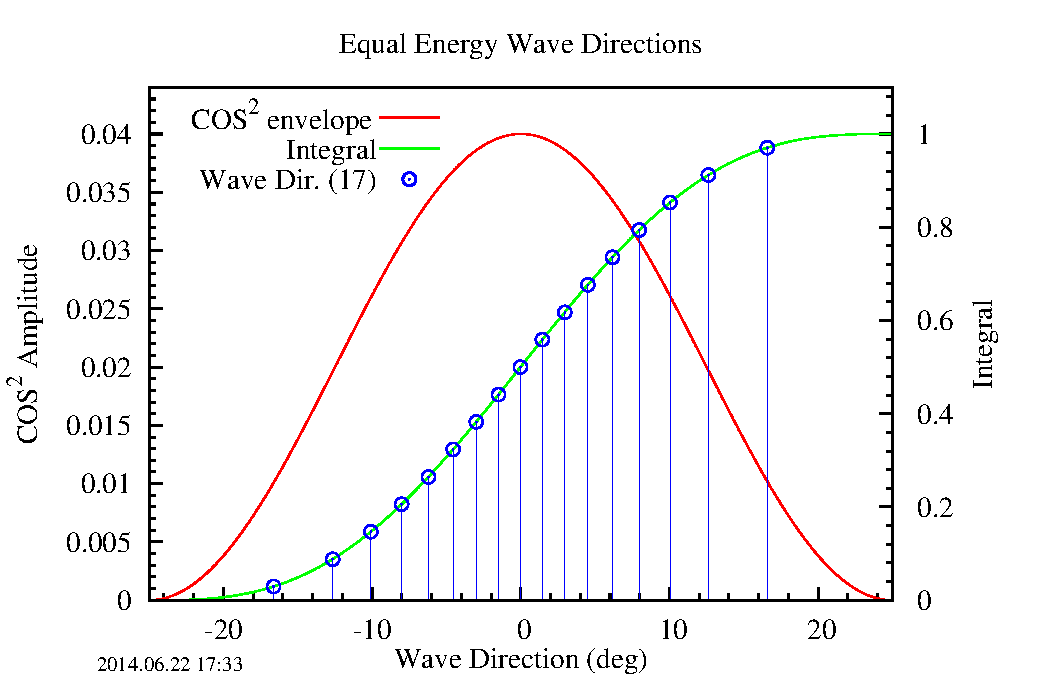
\includegraphics[width=.47\linewidth]{chaps/figures/WaveDirTest/WavesTest_001--equal_energy_disc.pdf}
   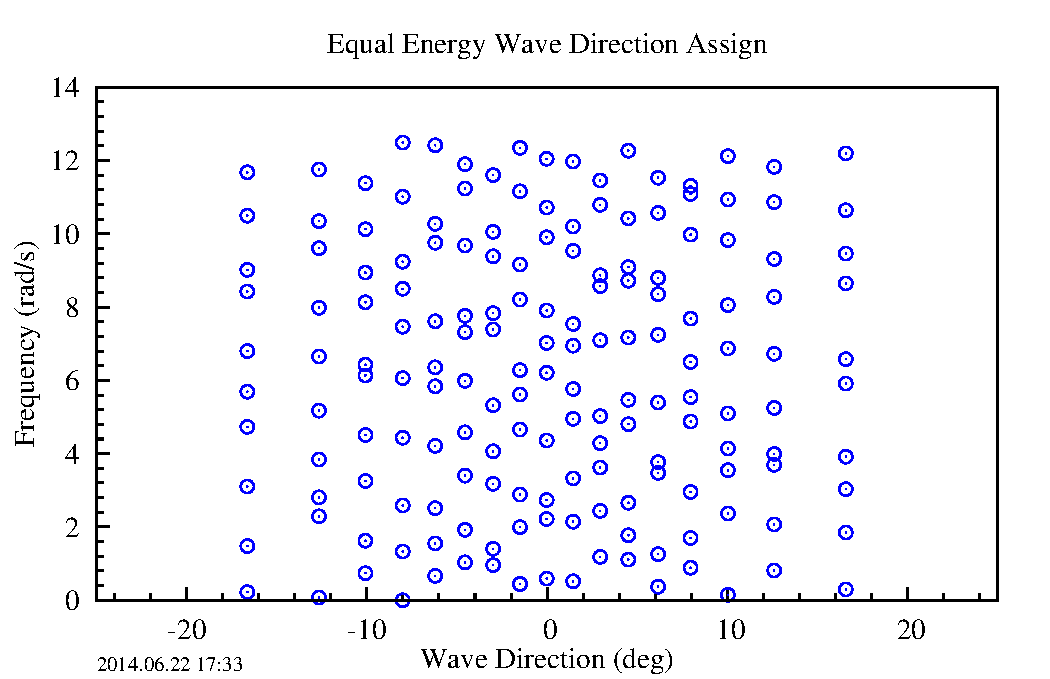
\includegraphics[width=.47\linewidth]{chaps/figures/WaveDirTest/WavesTest_001--wavedir_assign.pdf}
   \caption{Test case 001.  The right plot shows the randomly selected directions for each frequency.\label{fig:MultiDir:WavesTest001}}
\end{figure}

\begin{figure}
   \centering
   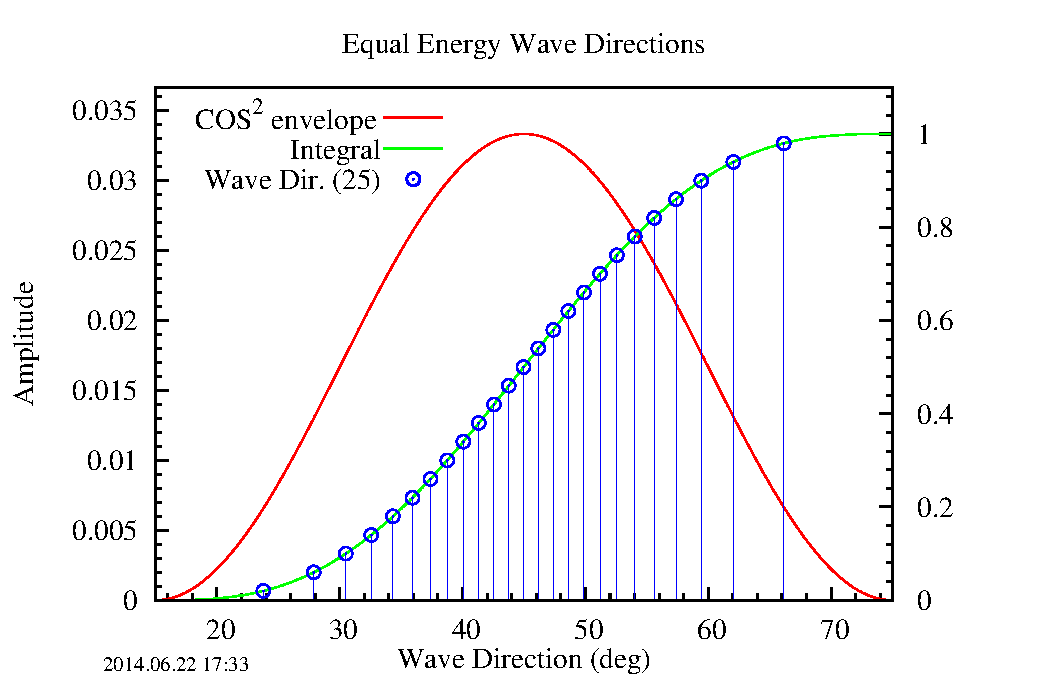
\includegraphics[width=.47\linewidth]{chaps/figures/WaveDirTest/WavesTest_002--equal_energy_disc.pdf}
   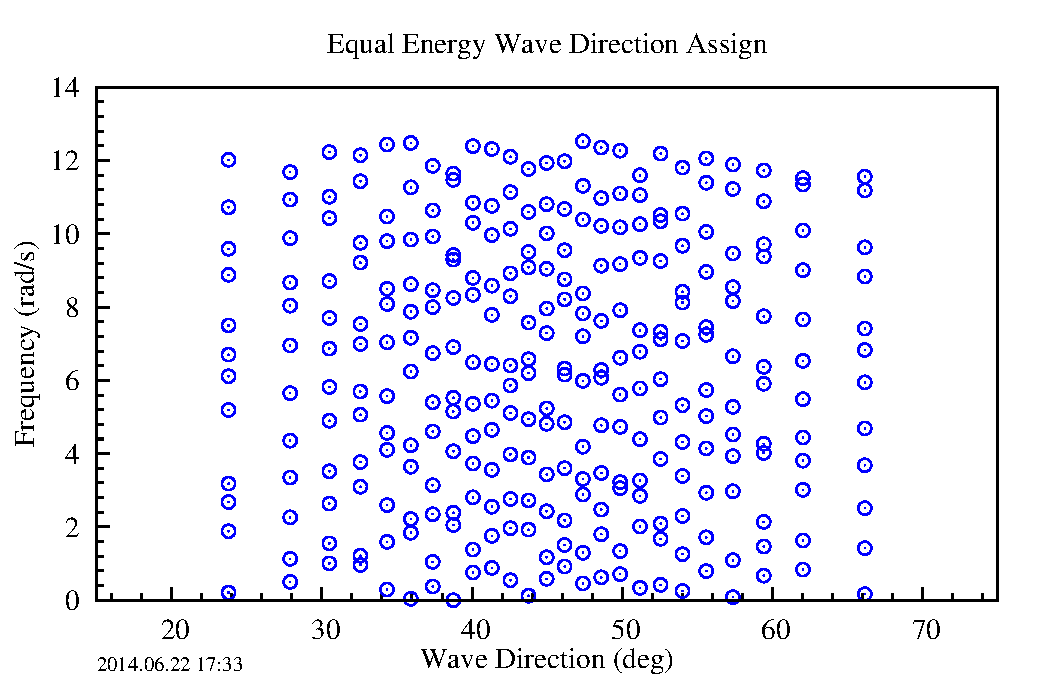
\includegraphics[width=.47\linewidth]{chaps/figures/WaveDirTest/WavesTest_002--wavedir_assign.pdf}
   \caption{Test case 002.  The right plot shows the randomly selected directions for each frequency.\label{fig:MultiDir:WavesTest002}}
\end{figure}

\begin{figure}
   \centering
   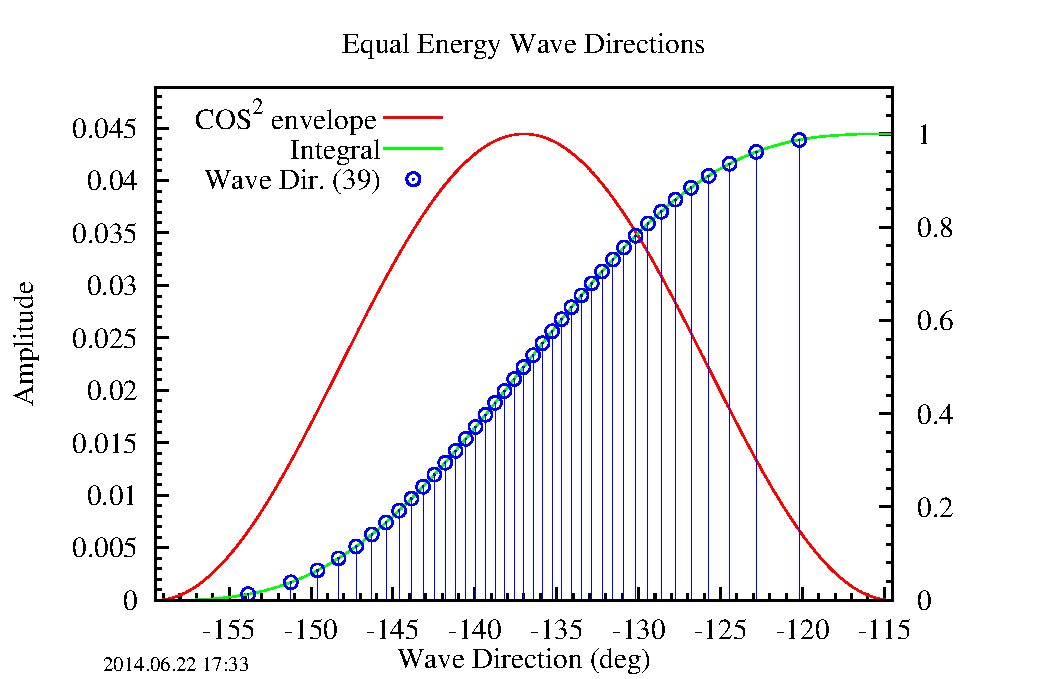
\includegraphics[width=.47\linewidth]{chaps/figures/WaveDirTest/WavesTest_003--equal_energy_disc.pdf}
   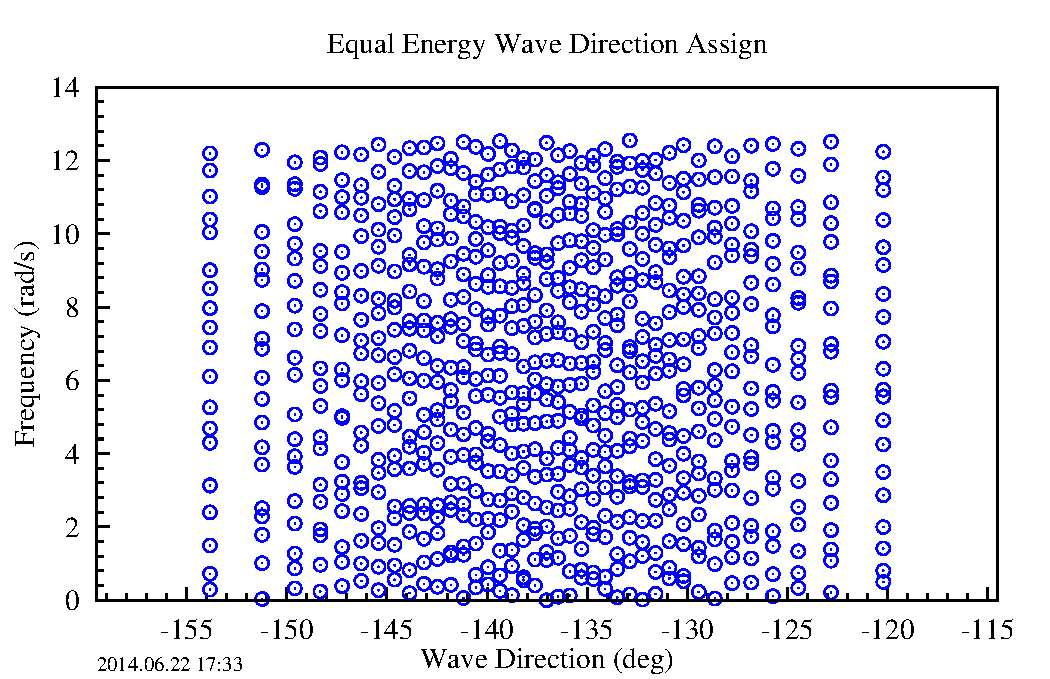
\includegraphics[width=.47\linewidth]{chaps/figures/WaveDirTest/WavesTest_003--wavedir_assign.pdf}
   \caption{Test case 003.  The right plot shows the randomly selected directions for each frequency.\label{fig:MultiDir:WavesTest003}}
\end{figure}

\begin{figure}
   \centering
   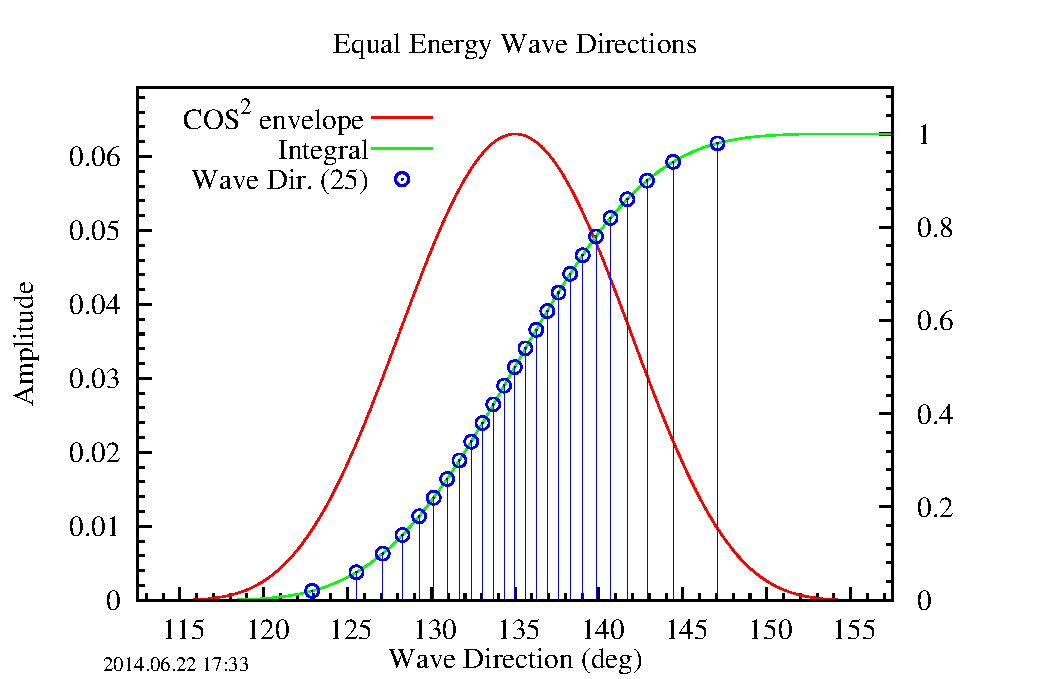
\includegraphics[width=.47\linewidth]{chaps/figures/WaveDirTest/WavesTest_004--equal_energy_disc.pdf}
   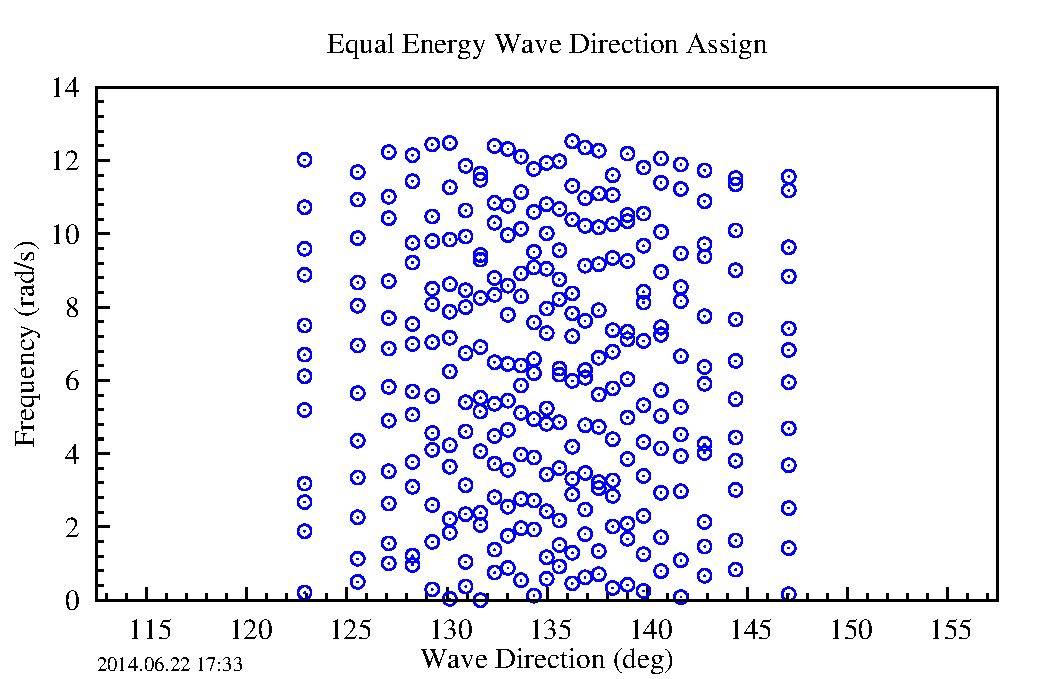
\includegraphics[width=.47\linewidth]{chaps/figures/WaveDirTest/WavesTest_004--wavedir_assign.pdf}
   \caption{Test case 004.  The right plot shows the randomly selected directions for each frequency.  This is the same as test case 002 with $\bar\theta=135$ and $S=2.3$.  Note that the ordering of the assigned frequencies is the same as in case 002.\label{fig:MultiDir:WavesTest004}}
\end{figure}

\begin{figure}
   \centering
   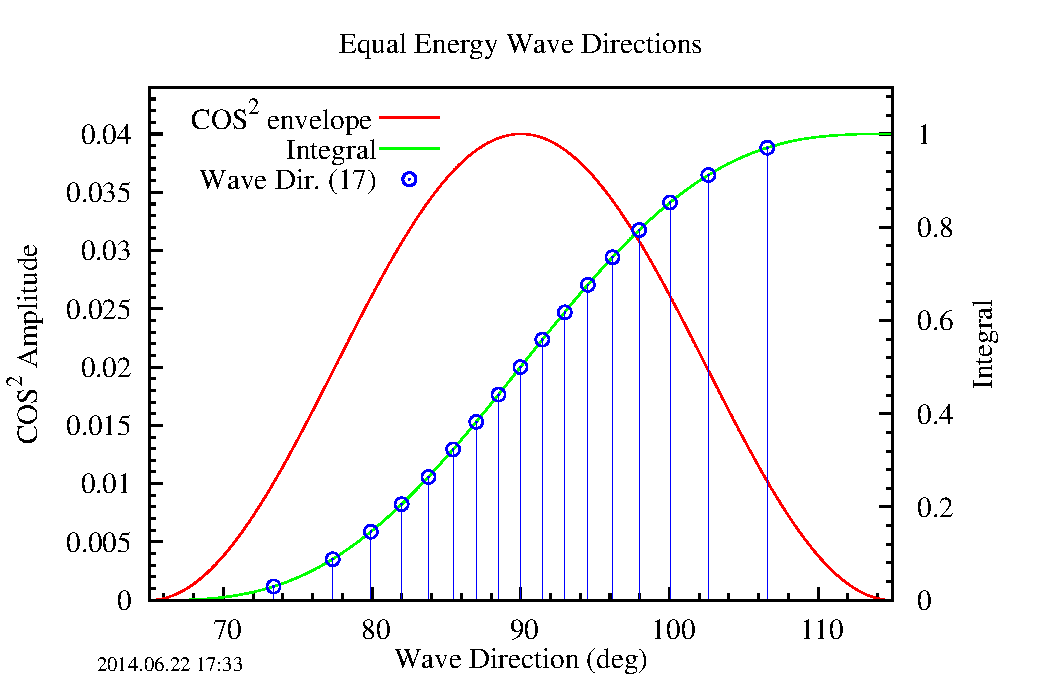
\includegraphics[width=.47\linewidth]{chaps/figures/WaveDirTest/WavesTest_005--equal_energy_disc.pdf}
   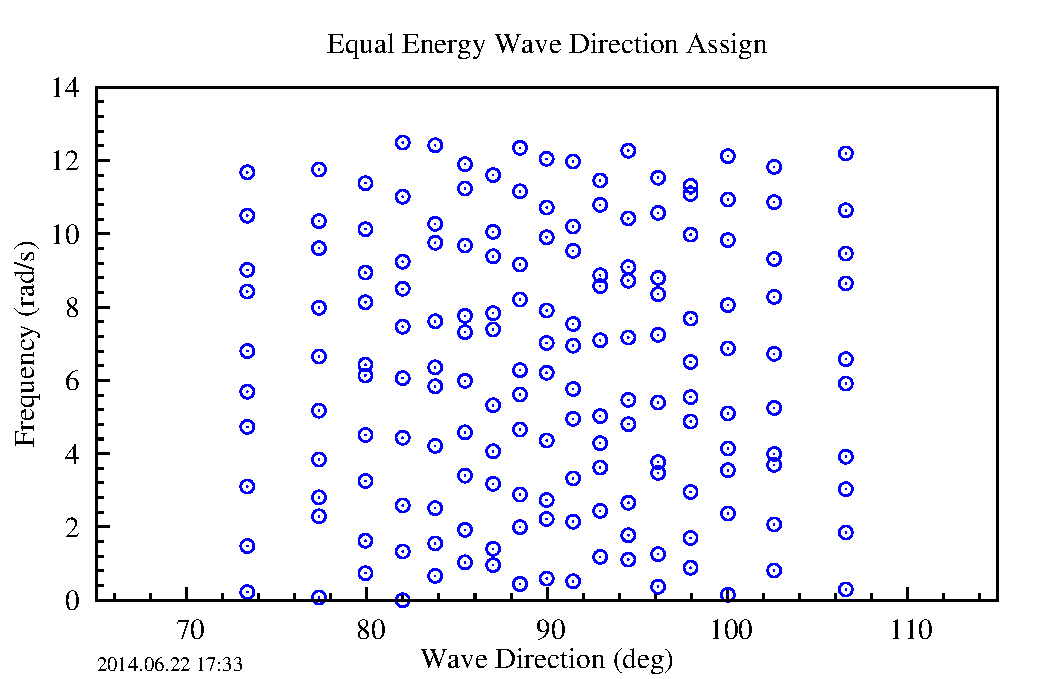
\includegraphics[width=.47\linewidth]{chaps/figures/WaveDirTest/WavesTest_005--wavedir_assign.pdf}
   \caption{Test case 005.  The right plot shows the randomly selected directions for each frequency.\label{fig:MultiDir:WavesTest005}}
\end{figure}

\begin{figure}
   \centering
   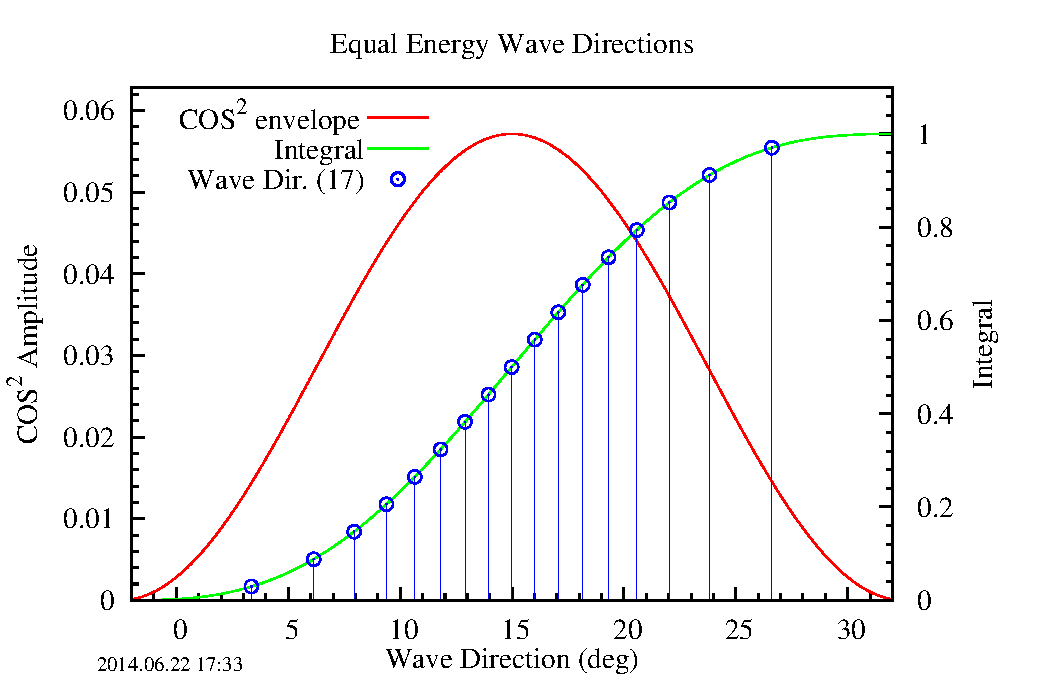
\includegraphics[width=.47\linewidth]{chaps/figures/WaveDirTest/WavesTest_008--equal_energy_disc.pdf}
   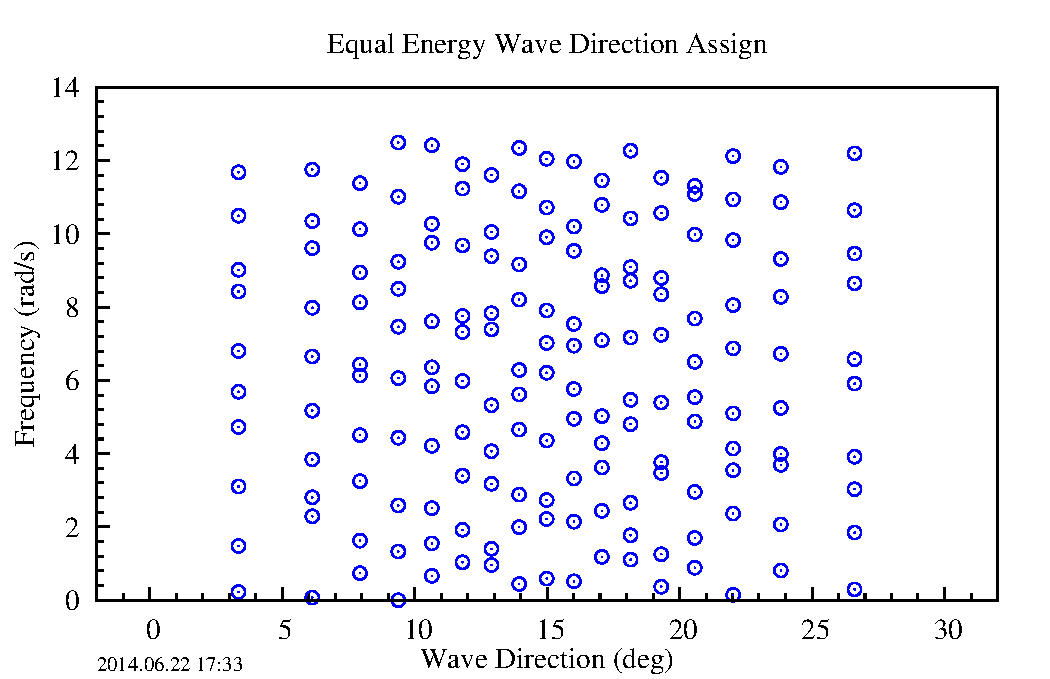
\includegraphics[width=.47\linewidth]{chaps/figures/WaveDirTest/WavesTest_008--wavedir_assign.pdf}
   \caption{Test case 008.  The right plot shows the randomly selected directions for each frequency.\label{fig:MultiDir:WavesTest008}}
\end{figure}



%\section{Modifications to wave velocity and acceleration equations}
%\label{sec:MultiDir:eqMods}
%
%Several of the equations used within the \modname{Waves} module are modified to accomodate the wavedirections as a function of frequency.  In Jason's dissertation, the $cos(\beta)$ and $sin(\beta)$ terms in equation 2-31a, 2-31b, 2-32a, and 2-32b are moved inside the IFFT.  %In the code, these are now implimented as %page 33 of dissertation 
%\begin{equation}
%v_1(t,X,Y,Z) = 
%\label{eq:MultiDir:WaveVelxi}
%\end{equation}


\clearpage
\section{Changes during implimentation}
\begin{description}
   \item[Waves module:]{\varname{InitOutputType\%WaveDir} will continue to contain the mean wave heading.  A new array \varname{InitOutputType\%WaveDirArr} will contain the direction headings for each wave elevation (same number of elements as \varname{WaveElevCO}).}
   \item[Waves module:]{For calculations of wave height, velocity, and acceleration away from the origin, modifications were made to split the wave into $x$ and $y$ components and calculate each separately (used to be single component along wave direction).}
   \item[Waves module:]{the equations for the wave velocity and acceleration used within the \modname{Waves} module are modified to accomodate the wavedirections as a function of frequency.  In Jason's dissertation, the $cos(\beta)$ and $sin(\beta)$ terms in equation 2-31a, 2-31b, 2-32a, and 2-32b are moved inside the IFFT.}  %In the code, these are now implimented as %page 33 of dissertation}
   \item[WAMIT module:]{Change wording about \varname{WaveDir} to correspond to the mean wave direction.  Add in a new variable \varname{WaveDirArr} to handle the directions for each frequency.}
   \item[WAMIT module:]{Change the code to use \varname{WaveDirArr} at each frequency.  This involved combining what had been two one-dimensional interpolations into a single two-dimensional interpolation scheme.}
\end{description}

In addition to the above changes, a new pair of input and output arrays were specified to allow for the calculation of the wave elevation at arbitrarily specified (X,Y) coordinates.  The input array, \varname{WaveElevXY}, of size $2\times N$ allows the for a set of $N$ arbitrary number of $(x,y)$ coordinates to be specified.  For this array, index 1 corresponds to specifies which coordinate ($x$ or $y$) and index 2 corresponds to point number.  If \varname{WaveElevXY} has been allocated at the gluecode or driver level, an array, \varname{WaveElevSeries}, of size \varname{NStepWave}$\times N$ is returned.  The first index of this array is the timestep (of the \varname{NStepWave} timesteps in the simulation), and the second index corresponds to the point number (of $N$ points) specified in the \varname{WaveElevXY} input array.  This has been implimented both within the \modname{Waves} module and within \HD itself.  It has been tested with the \HD driver and with the \modname{WAMIT2} driver code to generate sea surface movies corresponding to each of the 8 tests listed in \Cref{tab:MultiDir:Tests}.

%\end{document}



\maketitle

\pagenumbering{roman}
\setcounter{page}{3}

%\fancypagestyle{plain}
% ====================================================================
%    EXECUTIVE SUMMARY
% ====================================================================

%\newpage
%\chapter*{Executive Summary}
\addcontentsline{toc}{chapter}{Executive Summary}
This document reflects the planning and changes necessary to the HydroDyn codebase for the inclusion of second order forces and bi-directional waves. This document is a work in progress and will be continually updated until the second order forces and bi-directional waves have been included.  It also contains an overview of the architecture of the WAMIT2 code, and some specifics on the algorithm development.  In addition to this document, a set of documentation generated from the source code by Doxygen exists and provides more current information.   %FIXME: correct this once the document is completed

Adding second order forces and bi-directional waves will be done in two phases. In the first phase, a new sub-module, {\tt WAMIT2}, will be developed for the calculation of second order forces. This will include bi-directional waves at the start. In the second phase, bi-directional waves will be incorporated into the existing \HD codebase. This will entail changes to the HydroDyn module, and to the {\tt HydroDyn\_Input}, {\tt HydroDyn\_Output}, {\tt Waves}, and {\tt WAMIT} sub-modules. There may also be some slight changes to other pieces (unsure about {\tt Morrison}).



%\clearpage



\renewcommand{\contentsname}{Table of Contents}
\tableofcontents
\clearpage
\listoffigures
\listoftables
\clearpage
\todototoc
\clearpage
%\listofQuestion
%\listoftodos      %Note: this is a todo list of stuff to fix.
\clearpage
\pagenumbering{arabic}

%\fancypagestyle{fancy}





\chapter{Overview}
\label{chap:Overview}
This document serves two functions: first, as a guide to how second order forces and bi-directional waves should be incorporated into HydroDyn, and second to document the actual changes as they are made. While Tiago Duarte was visiting NREL over a 6 month period in 2012 and 2013, he sketched out in detail how to incorporate both second order effects and bi-directional waves into HydroDyn. This document is primarily based on his paper for the \emph{AIAA} SciTech 2014 conference\cite{duarte:2014}.

The second order forces can be developed in a standalone sub-module of HydroDyn called WAMIT2 following the FAST framework. This module will calculate the second order forces using information from the Waves sub-module, inputs from the HydroDyn module (including options from the input file), and data files produced by WAMIT. This module will be developed to use bi-directional waves, though testing will be somewhat limited due to the availability of a complete second order solution with bi-directional waves, in the form of a quadratic transfer function (QTF), produced by WAMIT.\footnote{Due to the complexity of the calculations, it has been estimated that a full QTF with 57 by 57 frequencies and 37 by 37 wave directions would take on the order of 52~years to calculate with our existing single threaded implimentation of WAMIT.}

The addition of bi-directional waves to HydroDyn will require modification of existing code. Since HydroDyn is still being developed, this addition will take place in the latter stages of the WAMIT2 module development. The bi-directional waves implimentation will use the equal energy approach outlined by Tiago in his document titled ``Multi-Directional Waves: Comparison and Implimentation.''

%FIXME:  Put in an explanation of the platform orientation constraints -- i.e.  it must be the same as calculated by WAMIT.
%        Put in other assumptions that must be necessary for this module to work.


%[Insert diagram of HydroDyn modifications from Tiago here -- from Multi- Directional Waves]



\chapter{Background information}
\label{chap:Background}
HydroDyn is currently undergoing a conversion to the FAST modularization framework. During this conversion, some additional capabilities are being added to HydroDyn including jacket platforms. At present, HydroDyn does not account for second order wave forces: those forces that arise from the sum and difference of the frequencies of incident waves. HydroDyn also only includes uni-directional waves where all waves are incident from the same direction.

At the start of a FAST simulation, HydroDyn is initialized and calculates the wave spectrum\footnote{
      The wave spectrum is complex-valued and therefore includes all the phase information, so the time history of the wave can be found easily through an FFT.}
and time history using the \emph{waves} sub-module.  This information is then used by the \emph{WAMIT} sub-module and a few other sub-modules to calculate the first order wave foreces on the platform.  Because the frequency, direction, and phase of each of the wave components is known at initialization, a time series of the second order forces can be calculated using the \emph{WAMIT2} sub-module before the simulations begins. This requires that the following assumptions are made:
\begin{itemize}
   \item{the wave information in frequency space is known before the start of the simulation (the time series can be found through an FFT),}
   \item{the time series of second order forces will act on a single point at the origin (as the first order forces do),}
   \item{wave forces and moments are fixed to a reference frame that translates (but does not rotate) with the platform,}
   \item{Wavelengths are large compared to the motion of the platform.}
\end{itemize}

\section{Platform Displacement and Rotation}
The complete timeseries for the forces and moments comprising the loads from the first and second order waves are calculated during the initialization of a FAST simulation.  These calculated loads are given at the platform origin in the platform rest reference frame and applied during the simulation.  During the simulation, the platform will translate and rotate as a result of these loads, aerodynamic loads, and other real time loads (mooring lines etc.).
The calculation of the first and second order wave loads do not take into account this displacement.  

During the simulation, the FAST glue code calls \HD to calculate the platform loads at each timestep.  Since the first- and second-order wave load timeseries were calculated during the initialization, these values are looked up at each timestep and reported back to the glue code on a point mesh (includes translation and rotation).



\endinput

The implication of this is that as the platform translates and rotates, the wave field and resulting loads are in effect translated and rotated with it.  For translation, this is not problematic since the translation is slow in comparison with the wave velocity.  However, it is not desirable to have the wave directionality also changing as the platform yaws, so an additional step is taken within \HD to compensate for the platform rotation before returning the forces and moments to the glue code.  This keeps the wave directionality and resulting moments in the inertial (non-rotated) reference frame of the platform.  This could potentially result in inaccuracies in response if the pitch and roll responses were dramatically different for waves incident along $x$ or $y$ respectively.




\endinput
FIXME: add figure from page 141 of notebook



Effectively means that the wave field and resulting loads move with the platform.  This is not likely to cause problems for surge and sway translation since the platform surge response tends to be slow in comparison with the wave velocity. There may be potential for issues with large heave displacements since WAMIT assumes the translational motions are \emph{small} compared to the wavelength during response force calculations.


   %\part{Multi-Directional Waves}
\chapter{Multi-directional Waves}
\label{chap:MultiDir}


In order to incorporate bi-directional waves, changes were made to the input files, how the data is stored internally, and to the computation of the first order forces. The second order forces were designed from the beginning to include bi-directional waves.

For our implimentation of the multi-directional waves, we are using the equal energy discretization which is used in the commercial code OrcaFlex.  With this method the same $N/2+1$ frequencies as used in the uni-directional case are used here.  A total of $\Theta$ (\varname{WaveNDir} in input file) discrete directions are used and each frequency is assigned to one of the discrete directions.
The value of $(\frac{N}{2}) / \Theta$ needs to be an integer so that each direction contains the same number of frequencies. $\Theta$ may need to be adjusted within the \modname{Waves} module to ensure this is true (see \Cref{sec:MultiDir:ThetaAdjust}).

\begin{center}
   \begin{minipage}[t]{\linewidth}
      \fvset{frame=single,fontsize=\scriptsize,numbers=left,numbersep=3pt,obeytabs,tabsize=1,fontfamily=fvm,commentchar=\%}
      \VerbatimInput{chaps/HD_Input/HD_Input_File_Waves.txt}
   \end{minipage}
   \captionof{table}{New section for the \HD input file for multi-directional waves.  This section is inserted where \emph{WaveDir} is currently defined.}
   \label{tab:HD_WAMIT2_InputModsWaveDir}
\end{center}


If $\varname{WaveDirMod}=1$, then a check is performed to make sure that $\varname{WaveMod}=$2, 3, or 4 (JONSWAP, white-noise, user defined).  If this is true, then an internal logical variable \varname{WaveMultiDir} is set to true and passed to modules that need to know about multiple wave directions.

Within the code in the \modname{HydroDyn\_Input} module, the maximum and and minimum directions actually used stored as \varname{WaveDirMin} and \varname{WaveDirMax}.  Since the wave direction assignments are performed using the equal energy approach, the actual maximum and minimum values will cover a smaller range than requested by the \varname{WaveDirRange} variable (see \Cref{sec:MultiDir:Testing}).
\begin{eqnarray}
   \varname{WaveDirMin} >& \varname{WaveDir} - \varname{WaveDirRange}/2\\
   \varname{WaveDirMax} <& \varname{WaveDir} + \varname{WaveDirRange}/2.
\label{eq:WaveDirMinMax}
\end{eqnarray}
These variables will be used in checking the WAMIT output files used (both first and second order).  Care should be taken to allow for crossing the $\pm \pi$ direction boundary.


\section{Adjusting $\Theta$ within the \modname{Waves} module}
\label{sec:MultiDir:ThetaAdjust}
To use the equal energy approach outlined below, $(\frac{N}{2}) / \Theta$ must be an integer, so it may be necessary to change $\Theta$ from the user specified value.  The difficulty with enforcing this arises from three requirements:
\begin{enumerate}
   \item{WaveNDir is odd in order to keep the center direction}
   \item{$N$ is adjusted by HydroDyn to be a product of smallish numbers for efficiency in the FFT\label{list:N}}
   \item{$(\frac{N}{2})/\Theta$ needs to be an integer to keep the energy distribution correct\footnote{Originally the requirement was set such that $(\frac{N}{2}-1)/\Theta$ was used (the $\omega=0$ frequency was ignored).  However, it was found that $(\frac{N}{2}-1)/\Theta$ was often a prime number, which would lead to user frustration.}}
\end{enumerate}
The third requirement means that $N/2$ is a product of integers such that $\Theta$ is one of them.  For small values of $\Theta$, this is unlikely to be an issue when $N$ is large, but could be problematic for short simulations where $N$ is smaller.\footnote{$N$ is initially set to \varname{TMax}/\varname{WaveDT} and then increased until it is the product of small numbers.}  For large values $\Theta$, it becomes less likely this would be true.  In order to satisfy these conditions, the value of $\Theta$ will be adjusted.\footnote{While it is theoretically possible to adjust $N$ such that the third condition is satisfied, this would have the undesirable consequence of changing the frequency step (see \Cref{eq:IFFT_N}).  This would in turn change the values of the complex wave amplitude in frequency space ($A_m$) for a given random number seed value.  Subsequently, the ability to reproduce the wave height and wave force timeseries for a given seed pair would not be preserved.}

For small values of $\Theta$, it may only be necessary to increase it slightly to satisfy the requirements (for example, change $\Theta=7$ to $\Theta=9$).  For large values of $\Theta$ (perhaps $>60$), it may be necessary adjust the value several times before a suitable value is found.  This could be done as outlined in \Cref{fig:Theta:Adjust}.  Note that we do not want to simply allow $\Theta$ to increase until a suitable value is found in the unlikely event that $N/2$ is a prime number.  In this case $\Theta$ will have to be increased until $\Theta=N/2$, which would mean each frequency has a unique wave heading and no binning occured.  This can only be corrected by having the user change \varname{WaveDT} or \varname{WaveTMax} since $N$ is adjusted internally to satisfy condition \ref{list:N}.
\begin{figure}
   \centering\begin{tikzpicture}

% Init
\node[process,text width=35mm] 
      (initialize)  {$\Theta_{init}=\Theta$\\ 
                     $\Theta_\text{max}=1.25\times \Theta_\text{init}$};

% odd?
\node[decision,below of=initialize,node distance=20mm]
      (odd) {Is $\Theta$ odd};
   \draw[cl] (initialize.south) -- (odd);

  % n branch
   \node[process,right of=odd,node distance=35mm,text width=25mm]
         (makeodd) { $\Theta=\Theta+1$\\
                     $\Theta_{init} = \Theta$\\
                     Warn user that it wasn't odd and new value.};
      \draw[cl] (odd) -- (makeodd) node[midway,above] {n};


% first check, continue
\node[decision,below of=odd,node distance=20mm,text width=20mm,inner sep=0pt]
      (CheckTheta1) {$(\frac{N}{2})/\Theta$\\integer};
   \draw[cl] (odd) -- (CheckTheta1) node[midway,left] {y};
   \draw[cl] (makeodd) -- (CheckTheta1);

   %y branch, done
   \node[process,text width=20mm]
         (Done1) at ($(CheckTheta1 -| makeodd)$)  {No change to $\Theta$};
      \draw[cl] (CheckTheta1) -- (Done1) node[midway,above] {y};
   % return
   \node[return,right of=Done1,node distance=25mm]
         (Return1) {Return};
      \draw[cl] (Done1) -- (Return1);

% not done, search up for solution
\node[process,below of=CheckTheta1,node distance=20mm]
      (Increase) {$\Theta=\Theta+2$};
   \draw[cl] (CheckTheta1) -- (Increase) node[midway,left] {n};

\node[decision,below of=Increase,node distance=20mm,text width=20mm,inner sep=0pt,font=\footnotesize]
      (ThetaLimitUpper) {$\Theta < \Theta_\text{max}$};
   \draw[cl] (Increase) -- (ThetaLimitUpper);

   % if still within range, check value
   \node[decision,right of=ThetaLimitUpper,node distance=45mm,text width=20mm,inner sep=0pt]
         (CheckTheta2) {$(\frac{N}{2})/\Theta$\\integer};
      \draw[cl] (ThetaLimitUpper) -- (CheckTheta2) node[midway,above] {y};

   % if we have an answer, done and return.  If not, loop again
   \node[process,right of=CheckTheta2,node distance=40mm,text width=25mm]
         (Finish) {Tell user what $\Theta$ is and why};
      \draw[cl] (CheckTheta2) -- (Finish) node[midway,above] {y};
      % Return
      \node[return,right of=Finish,node distance=25mm]
            (Return2) {Return};
         \draw[cl] (Finish) -- (Return2);
      % or loop again
      \draw[cl] (CheckTheta2) |- (Increase) node[midway,below left] {n};

%%% --- Don't go down.  We only want to increase resolution, not decrease it.
%% didn't find solution before getting too big
%\node[process,below of=ThetaLimitUpper,node distance=20mm]
%      (Decrease) {$\Theta=\Theta_{init}-2$};
%   \draw[cl] (ThetaLimitUpper) -- (Decrease) node[midway,left] {n};
%
%\node[decision,below of=Decrease,node distance=20mm,text width=20mm,inner sep=0pt,font=\footnotesize]
%      (ThetaLimitLower) {$\Theta > \Theta_{init} \cdot (1.0-\Delta\Theta_\text{allow})$};
%   \draw[cl] (Decrease) -- (ThetaLimitLower);
%
%   % if still within range, check value
%   \node[decision,text width=20mm,inner sep=0pt]
%         (CheckTheta3) at ($(ThetaLimitLower)!.5!(ThetaLimitLower -| CheckTheta2)$) {$(\frac{N}{2})/\Theta$\\integer};
%      \draw[cl] (ThetaLimitLower) -- (CheckTheta3) node[midway,above] {y};
%      % if we do have an answer, retun
%      \draw[cl] (CheckTheta3) -| (Finish) node[midway,above left] {y};
%      % if not, loop again
%      \draw[cl] (CheckTheta3) |- (Decrease) node[midway,below left] {n};

% exceeded limit before finding solution
\node[process,below of=ThetaLimitUpper,node distance=27mm,text width=40mm]
      (NoSolution) {No Solution in range:\\$\Theta_\text{init} \rightarrow \Theta_\text{max}$\\Try changing $\Theta$ or \varname{WaveTMax}};
   \draw[cl] (ThetaLimitUpper) -- (NoSolution) node[midway,left] {n};

\node[return,right of=NoSolution,node distance=60mm,text width=40mm]
      (Return3) {Fatal Error: Return suggested value of WaveNDir if exists};
   \draw[cl] (NoSolution) -- (Return3);




\end{tikzpicture}
\endinput



\end{tikzpicture}
\endinput

%inputs from file
\node[process,below of=p1]
      (p2)  {Read input from file (and check)};
   \draw[cl] (p1) -- (p2);
   \draw[cl] (p2.south west) .. controls +(-4mm,-4mm) and +(-4mm,4mm) .. (p2.north west) node[midway,sloped,above,yshift=-1mm,font=\scriptsize] {NumCases};

% return
\node[return,below of=p2] (r1) {Return};
   \draw[cl] (p2) -- (r1);

\end{tikzpicture}

   \caption[Flowchart of how to find a suitable value of $\Theta$]{Flowchart of how to find a suitable value of $\Theta$ such that $(\frac{N}{2})/\Theta$ is an integer.  The reason for suggesting that \varname{WaveTMax} should be changed is that there is a possibility that $N/2$ is a prime number.  This is implimented at the start of the initialization subroutine of the \modname{Waves} module if multidirectional waves are selected.\label{fig:Theta:Adjust}}  
\end{figure}
 



\section{Equal Energy Approach}
\label{sec:MultiDir:EqEnergy}


\begin{table}[H]
   \centering
   \caption[Notation for multi-directional wave equations]{Notation for multi-directional wave equations.\label{tab:MultiDirWaves:Notation}}
   \begin{tabular}{cclc}
      \toprule
         Variable                   &  Variable Name           &  Description                            &  Units    \\
      \midrule
         $\Theta$                   &  \varname{WaveNDir}      &  User defined number of wave directions &   -       \\
         $\theta$                   &                          &  Current wave direction                 &  degrees  \\
         $\bar\theta$               &  \varname{WaveDir}       &  Central (mean) wave direction          &  degrees  \\
         $\delta\theta$             &  \varname{WaveDirRange}  &  Range of wave directions (full width)  &  degrees  \\
         $S$                        &  \varname{WaveDirSpread} &  Spreading function coefficient (1 typ) &   -       \\
      \bottomrule
   \end{tabular}
\end{table}




This method to simulate multi-directional waves assigns each frequency component of the wave to one of $\Theta$ discrete wave directions.  Each wave direction will have the same number of frequencies, $(\frac{N}{2})/\Theta$, assigned to it.  In order to preserve the energy distribution in the wave spreading function, the wave directions are assigned so that a greater number of directions are concentrated near the central frequency.

This method is only valid if the equation describing the total spectrum is separable into the frequency and direction parts as follows:
\begin{equation}
   S(\omega,\theta) = \bar{S}(\omega) \cdot D(\theta).
\label{eq:totalspectrum}
\end{equation}

The wave spreading function is given by
\begin{equation}
   D(\theta)   = C \left| \cos\left(\frac{\pi \: (\theta - \bar\theta)}{\delta \theta}\right) \right|^{2S},
\label{eq:WaveSpread}
\end{equation}
where the normalization constant, $C$, is given by
\begin{equation}
   C = \frac{\sqrt{\pi} \: \Gamma(S+1)}{\delta\theta \: \Gamma(S+1/2)},
\label{eq:WaveSpread:Const}
\end{equation}
and $\Gamma$ is the gamma function.
The spreading function should satisfy the normalization condition of
\begin{equation}
   \int\limits^{\bar\theta+\delta\theta/2}_{\bar\theta-\delta\theta/2} D(\theta) \, \mathrm{d}\theta \equiv 1.
\label{eq:WaveSpread:Norm}
\end{equation}
The cumulative energy distribution within the wave spreading function up to angle $\theta$ is given by
\begin{equation}
   P(\theta) = \int\limits^{\theta}_{\bar\theta - \delta\theta/2} D(\theta') \: \mathrm{d}\theta'.
\label{eq:WaveSpread:Energy}
\end{equation}

The following method may be used to set the appropriate wave directions to satisfy the equal energy approach.
\begin{enumerate}
   \item{Discretize the wave direction range $\delta\theta$ by $n_d$ steps and calculate $D(\theta)$ spreading function.  Set $n_d$ to a sufficiently large number such that the function is smooth enough for interpolation over $\Theta$ directions (set $n_d = 3 \Theta$).\label{list:EqEnergySolve:1}}
   \item{While calculating $D(\theta)$, calculate the cumulative energy sum up to the current direction as $P(\theta)$.}
   \item{Discretize $P(\theta)$ into $\Theta$ steps from $1/\Theta \leq P_i \leq 1-1/\Theta$.  Interpolate the function $D(\theta)$ found in step \ref{list:EqEnergySolve:1} to find the corresponding values of $\theta_i$.  The $\theta_i$ values are the wave directions used in the equal energy method.}
   \item{Randomly assign each of the $N/2$ frequencies (ignoring the end frequencies at which the wave amplitude is defined as zero) to a $\theta_i$ direction such that each wave direction has $(N/2)/\Theta$ frequencies assigned to it. \emph{This is the tricky bit to do such that the assignments are the same given a certain random number seeed pair.}}   % randomly assign to wave bins in groups of \Theta frequency sets.
\end{enumerate}

\subsection{A few notes}
There are a few things to take note of in this process.  First, in order to preserve the equal energy distribution within the wave direction spreading function, care must be taken so that $(N/2)/\Theta$ is an integer (see \Cref{sec:MultiDir:ThetaAdjust} for caveats with using a user defined value for $\Theta$).  Second, if it is desirable to have a greater number wave directions, it is preferable to increase $\Theta$ substantially.  Alternatively, the $\theta_i$ values could be treated as wave direction bins spanning a range of $\theta$ directions rather than a single direction.  The danger with this is that the distribution of random wave directions within the bin will affect the overall energy distribution of the spreading function.  A shaping function would then need to be applied to the bin to distribute wave directions within it.  In this case it would be preferable to increase $\Theta$ significantly in order to allow for more wave directions while preserving the energy distribution in the wave spreading function.  Short tests using MATLAB code indicate that a value of $\Theta = 399$ works well for allowing a seemingly random set of wave directions.  In practice, it may be preferable to keep $\Theta < 50$ for a more physical description of wave directionality.

%NOTE: there is a discrepency between this approach and what OrcaFlex does.  See page 155 of the version 9.7a manual.  In the OrcaFlex approach, the wave amplitude is held constant, and the frequency spacing is changed so as to preserve the energy content on the amplitude vs. frequency spectrum.  Our implimentation is slightly different in that we have a uniform $\Delta\omega$ and vary the amplitude.

\subsection{Implimentation and Testing}
\label{sec:MultiDir:Testing}

\paragraph*{Development testing}
During the implimentation of the multidirectional waves within the \modname{Waves} module, testing was performed to ensure that no errors were introduced into the equations used to calculate the wave elevation, velocity, and acceleration.  The following sequence was used to impliment the multidirectional waves within the waves module.
\begin{enumerate}
   \item{Add code section to change the value of \varname{WaveNDir}.  This was originally implimented such that $(\frac{N}{2}-1)/\Theta$ was an integer.  This was later changed when it was discovered that $(\frac{N}{2}-1)$ is often a prime number (due in part to how \varname{NStepWave} is adjusted -- see \Cref{sec:MultiDir:ThetaAdjust} for details). This code was tested before proceeding.}
   \item{Split the main loop over \varname{NStepWave2} frequencies.  The wave direction assignment loop is inserted between the first loop where the wave amplitudes and phases are assigned, and the second loop where the IFFTs are setup and performed.  Testing was performed to ensure that all the information necessary in the second loop existed.}
   \item{Create the wave direction assignment loop.  Some temporary print statements were used to output the wave direction information for plotting.  These results are shown in \Crefrange{fig:MultiDir:WavesTest001}{fig:MultiDir:WavesTest008}.}
   \item{The code necessary for processing the input array \varname{WaveElevXY} and return array \varname{WaveElevSeries} was developed at the \modname{Waves} module and the \modname{WAMIT2} driver level.  The subroutine for calculating the wave elevation at a specified $(x,y)$ coordinate was developed.  Movies were then created of the test cases listed in \Cref{tab:MultiDir:Tests} to verify that the wave elevation calculations were working correctly (it too some iterating to get this working).}
   \item{The code was then rearranged and modified so that the \varname{WaveElevXi}, \varname{WaveElevYi} elevation data uses the wave elevation routine.}
   \item{Now the wave velocity and acceleration equations were modified.  In the original calculations, the wave direction was handled after the FFT.  This was revised so that the wave direction was handled before the FFT was calculated.  Testing of this was performed by setting \varname{WaveNDir} = 1 and repeating a few CertTests that had been generated with the previous version of the \modname{Waves} module.  The results agreed to within the precision used for outputting the CertTest results.}
\end{enumerate}

At this point, it was concluded that the \modname{Waves} module was working as well as it had been prior to the implimentation of multi-directional waves.  A minor usability issue became apparent at this point regarding how \varname{WaveNDir} was adjusted within the code.  The decision was then made to modify the code such that we include the $\omega = 0$ term in the wave direction assignment.  This means that we now force $(\frac{N}{2})/\Theta$ to be an integer.  We also included code to give the user some idea of what values of \varname{WaveNDir} might work with their currently defined values of \varname{WaveTMax} and \varname{WaveDT}.

For testing the multi-directional waves there is one more test we can perform.  This is to check the correlation of the wave elevation at various $(x,y)$ locations.  This has not been performed yet.\todo{do this}



\paragraph*{Test Cases}
Multidirectional waves using the method described above are implimented within the \modname{Waves} module of \HD.  It is evaluated after the generation of the wave spectrum (JONSWAP or other).  The directions are assigned in groups of $\Theta$ frequencies so that one each frequency within the group is assigned a unique direction.  This is repeated for all $(N/2)/\Theta$ groups of frequencies.

Several test cases were performed to verify that the assignment of wave directions by frequency was correctly performed.  In each of the test cases listed in \Cref{tab:MultiDir:Tests}, a compiled version of the code with partially implimented modifications to the \modname{Waves} module was executed.  The calculated spreading function, integrated power of the spreading function, calculated wave directions, and the assigned wave directions were output using appropriately placed print statements (this was merely intended as an intermediate testing of the code, not a test that would be needed in this form later).  The results were plotted using gnuplot.

Tests numbered 002 and 004 are very similar with the only differences in $\bar\theta$, the mean wave direction, and $S$, the spreading coefficient.  A comparison of \Cref{fig:MultiDir:WavesTest002} and \Cref{fig:MultiDir:WavesTest004} shows the repeatablility during the assignment of the wave direction for each frequency: in each test, the $n^\text{th}$ frequency is assigned to the same wave direction index.  Though the frequencies are randomly assigned, the same seed was used in each of these tests and the random number generator had the same number of calls for wave amplitude prior to the assignment of the directions.

Tests numbered 001, 005, and 008 are identical with the exception of the mean wave direction.  Test 001 is oriented with the mean wave direction along the $x$ axis, and test 005 is oriented with the mean wave direction along the positive $y$ axis.  A movie of the sea surface for these two tests is useful in checking that the coordinate transformations are working correctly.

\begin{table}
   \centering
   \caption[Multi-directional waves test cases]{Multi-directional waves test case parameters.\label{tab:MultiDir:Tests}}
%   \tabcolsep=1.75mm
   \begin{tabular}{cccccccccc}
      \toprule
 Test Case  & \varname{WaveDirMod}&$\bar\theta$ &  $\delta\theta$ &  $S$   &  $\tau_\text{max}$ &  $\Delta\tau$   &  $N/2$ &  $\Theta$ &  $\frac{N/2}{\Theta}$  \\
  (-)       &                 &  (deg)          &  (deg)          &  (-)   &  (s)               &  (s)            &  (-)   &  (-)      &  (-)                     \\
      \midrule
   001      &      1          &    0            &   50            &  1.0   &   85               &  0.25           &  170   &  17       &  10                      \\
   002      &      1          &   45            &   60            &  1.0   &  150               &  0.25           &  300   &  25       &  12                      \\
   003      &      1          & -137            &   45            &  1.0   &  390               &  0.25           &  780   &  39       &  20                      \\
   004      &      1          &  135            &   45            &  2.3   &  150               &  0.25           &  300   &  25       &  12                      \\
   005      &      1          &   90            &   50            &  1.0   &   85               &  0.25           &  170   &  17       &  10                      \\
   006      &      0          &   45            &   60            &  1.0   &  150               &  0.25           &  300   &  --       &  --                      \\
   007      &      0          & -137            &   45            &  1.0   &  390               &  0.25           &  780   &  --       &  --                      \\
   008      &      1          &   15            &   35            &  1.0   &   85               &  0.25           &  170   &  17       &  10                      \\
      \bottomrule
   \end{tabular}
\end{table}


\begin{figure}
   \centering
   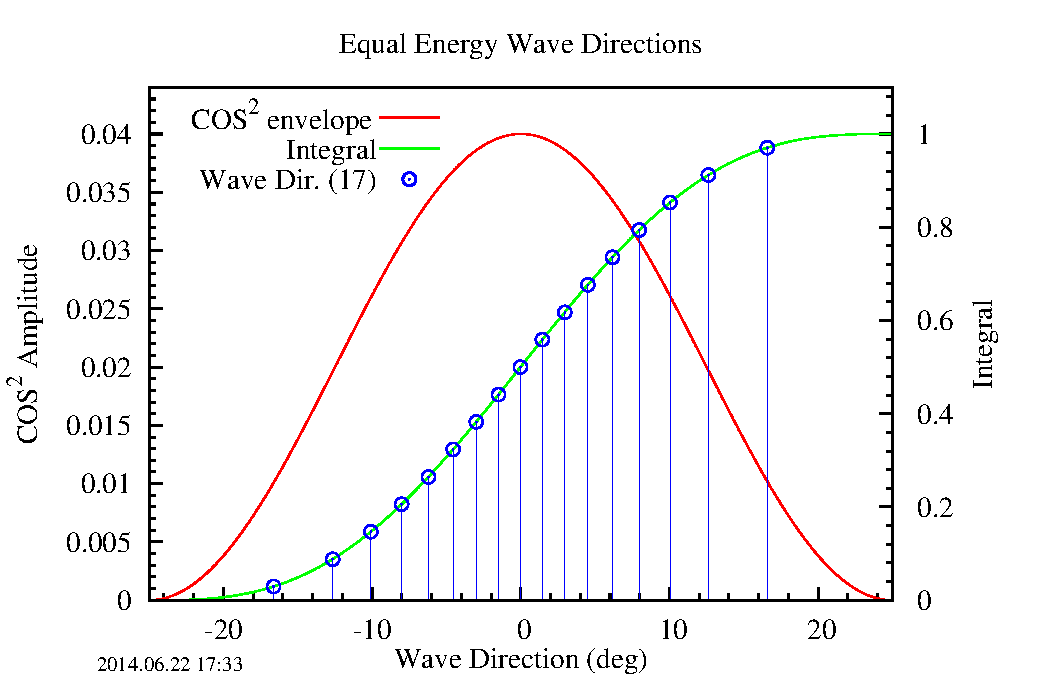
\includegraphics[width=.47\linewidth]{chaps/figures/WaveDirTest/WavesTest_001--equal_energy_disc.pdf}
   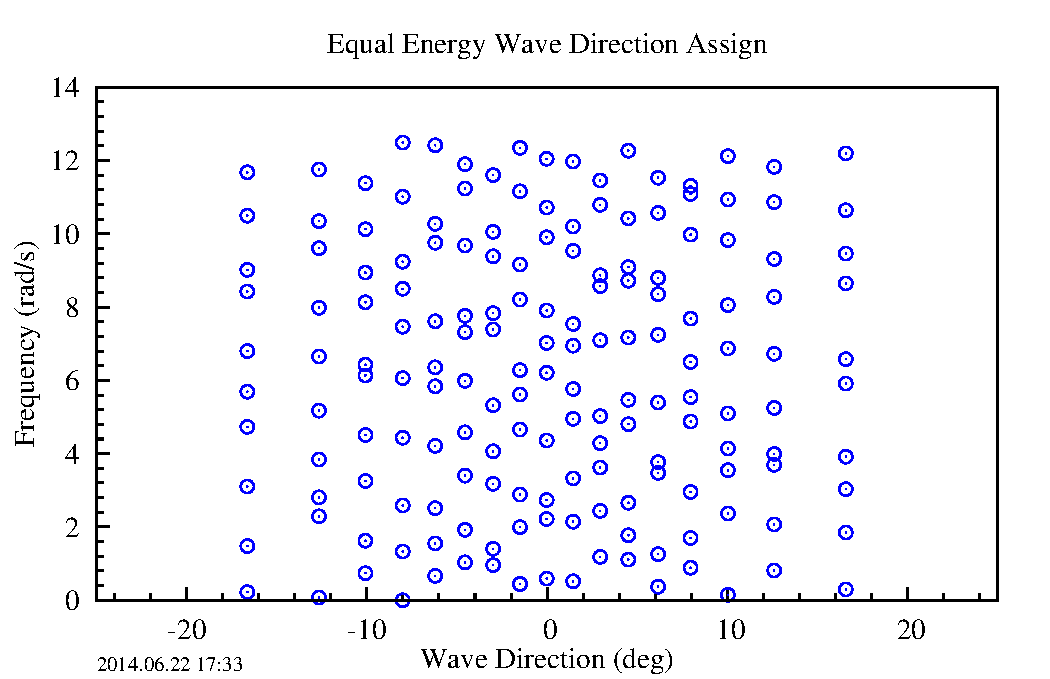
\includegraphics[width=.47\linewidth]{chaps/figures/WaveDirTest/WavesTest_001--wavedir_assign.pdf}
   \caption{Test case 001.  The right plot shows the randomly selected directions for each frequency.\label{fig:MultiDir:WavesTest001}}
\end{figure}

\begin{figure}
   \centering
   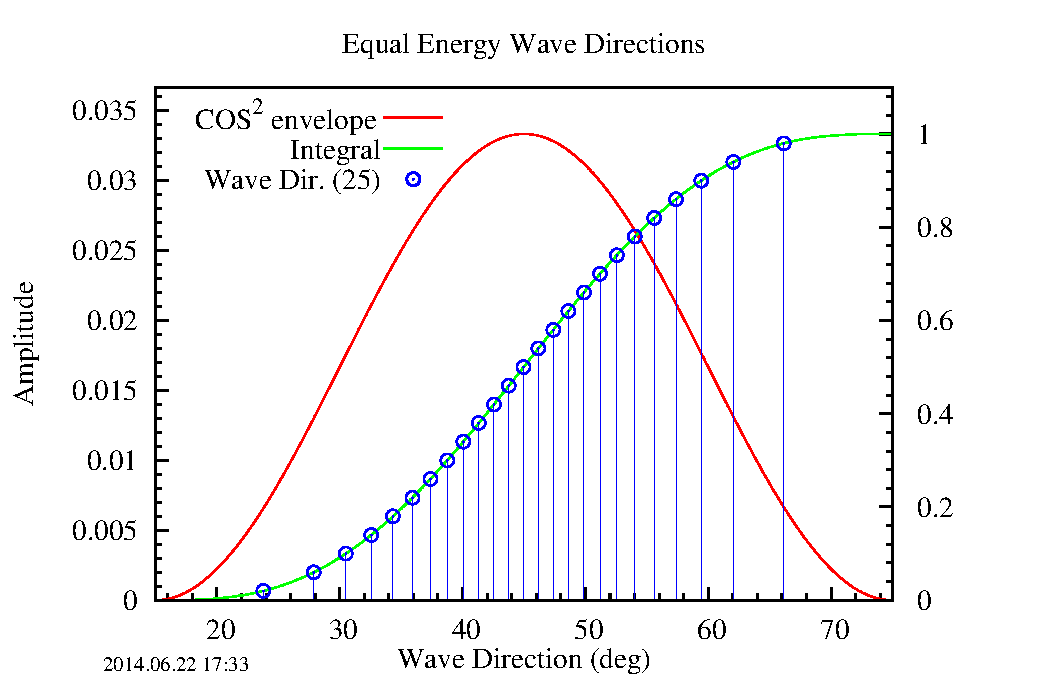
\includegraphics[width=.47\linewidth]{chaps/figures/WaveDirTest/WavesTest_002--equal_energy_disc.pdf}
   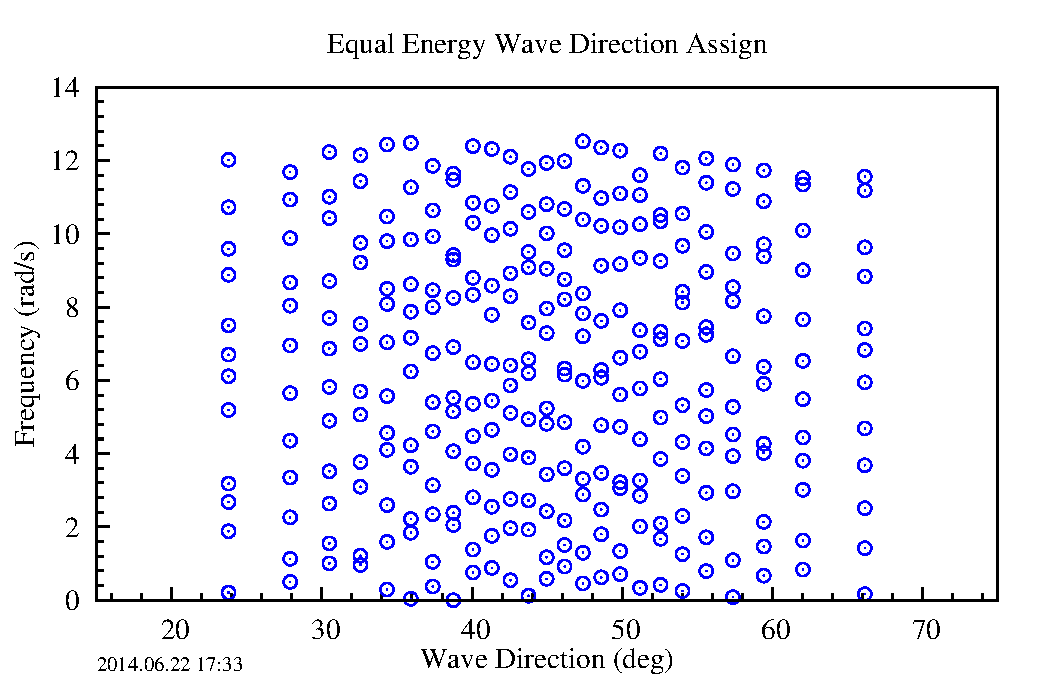
\includegraphics[width=.47\linewidth]{chaps/figures/WaveDirTest/WavesTest_002--wavedir_assign.pdf}
   \caption{Test case 002.  The right plot shows the randomly selected directions for each frequency.\label{fig:MultiDir:WavesTest002}}
\end{figure}

\begin{figure}
   \centering
   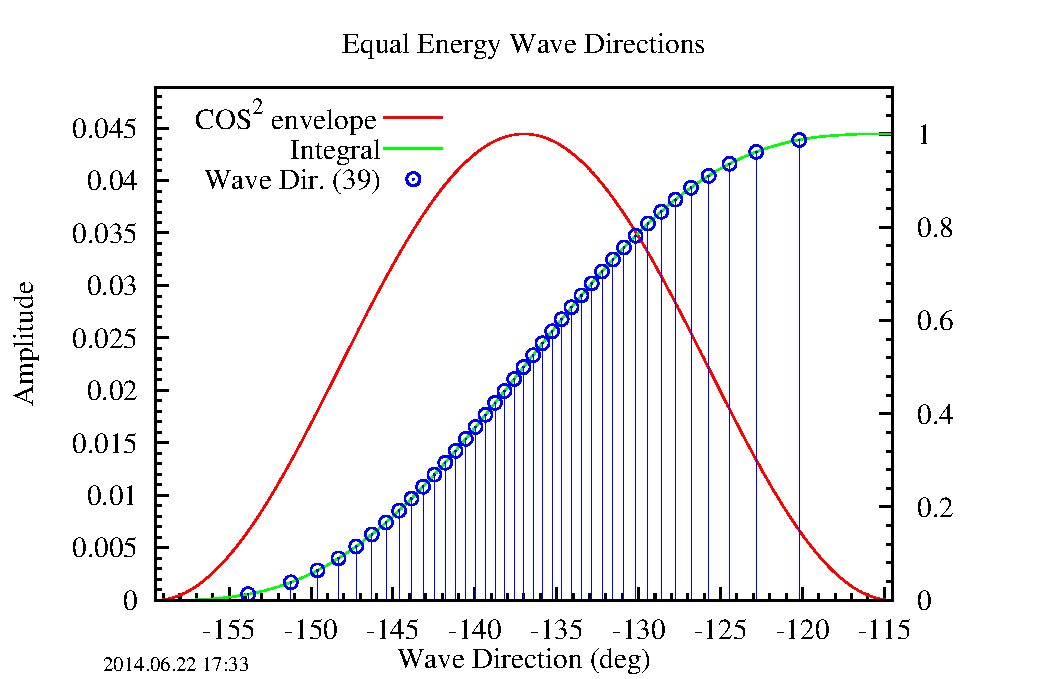
\includegraphics[width=.47\linewidth]{chaps/figures/WaveDirTest/WavesTest_003--equal_energy_disc.pdf}
   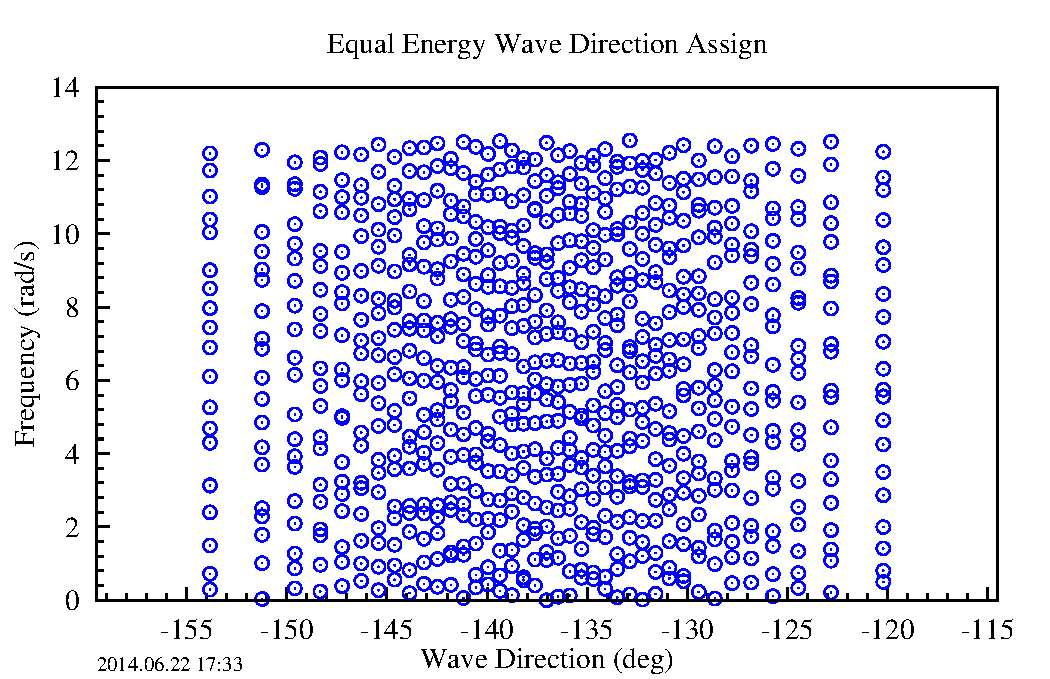
\includegraphics[width=.47\linewidth]{chaps/figures/WaveDirTest/WavesTest_003--wavedir_assign.pdf}
   \caption{Test case 003.  The right plot shows the randomly selected directions for each frequency.\label{fig:MultiDir:WavesTest003}}
\end{figure}

\begin{figure}
   \centering
   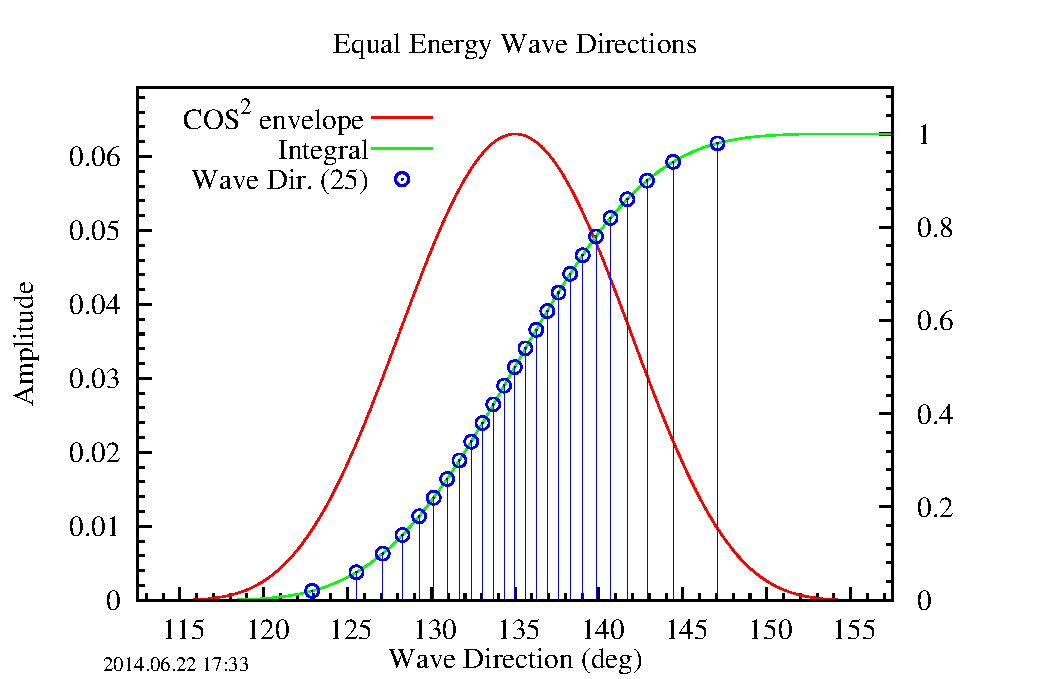
\includegraphics[width=.47\linewidth]{chaps/figures/WaveDirTest/WavesTest_004--equal_energy_disc.pdf}
   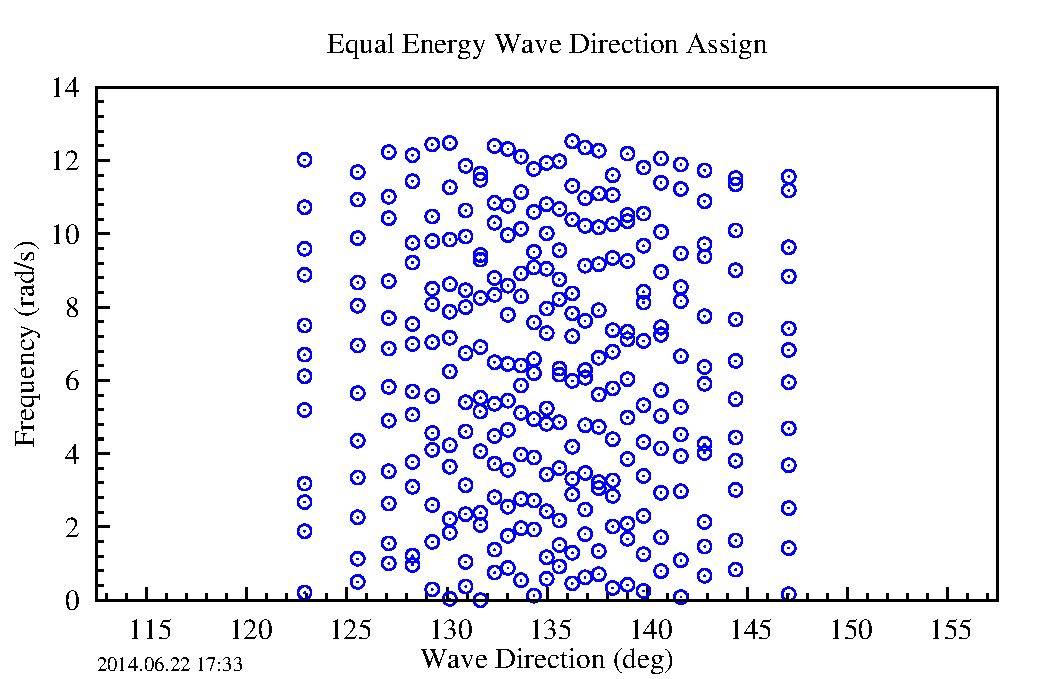
\includegraphics[width=.47\linewidth]{chaps/figures/WaveDirTest/WavesTest_004--wavedir_assign.pdf}
   \caption{Test case 004.  The right plot shows the randomly selected directions for each frequency.  This is the same as test case 002 with $\bar\theta=135$ and $S=2.3$.  Note that the ordering of the assigned frequencies is the same as in case 002.\label{fig:MultiDir:WavesTest004}}
\end{figure}

\begin{figure}
   \centering
   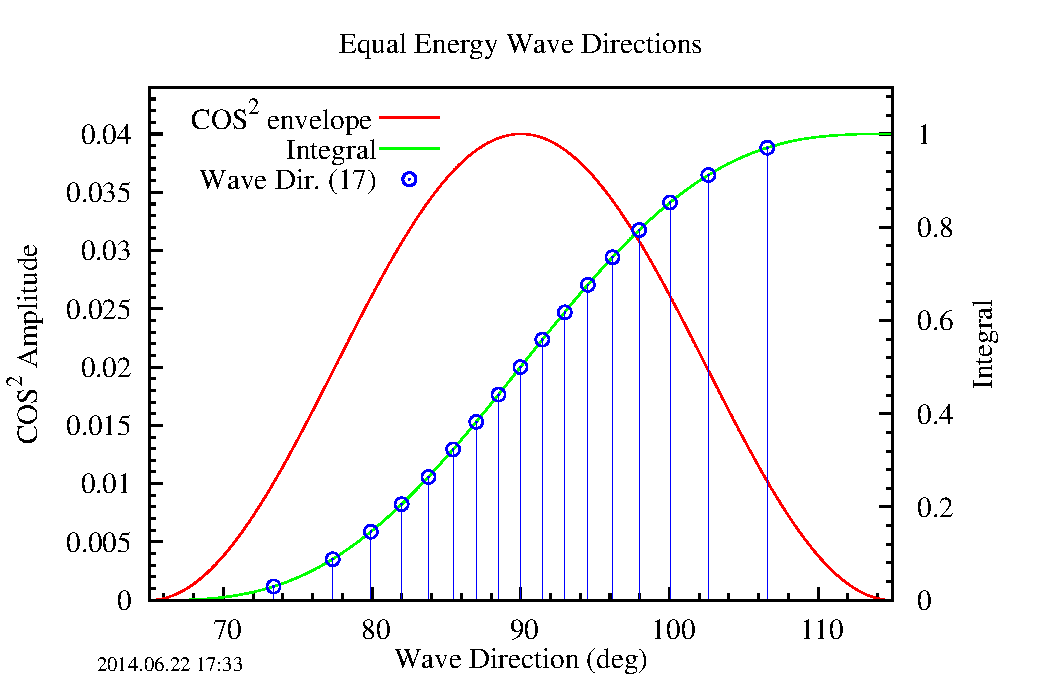
\includegraphics[width=.47\linewidth]{chaps/figures/WaveDirTest/WavesTest_005--equal_energy_disc.pdf}
   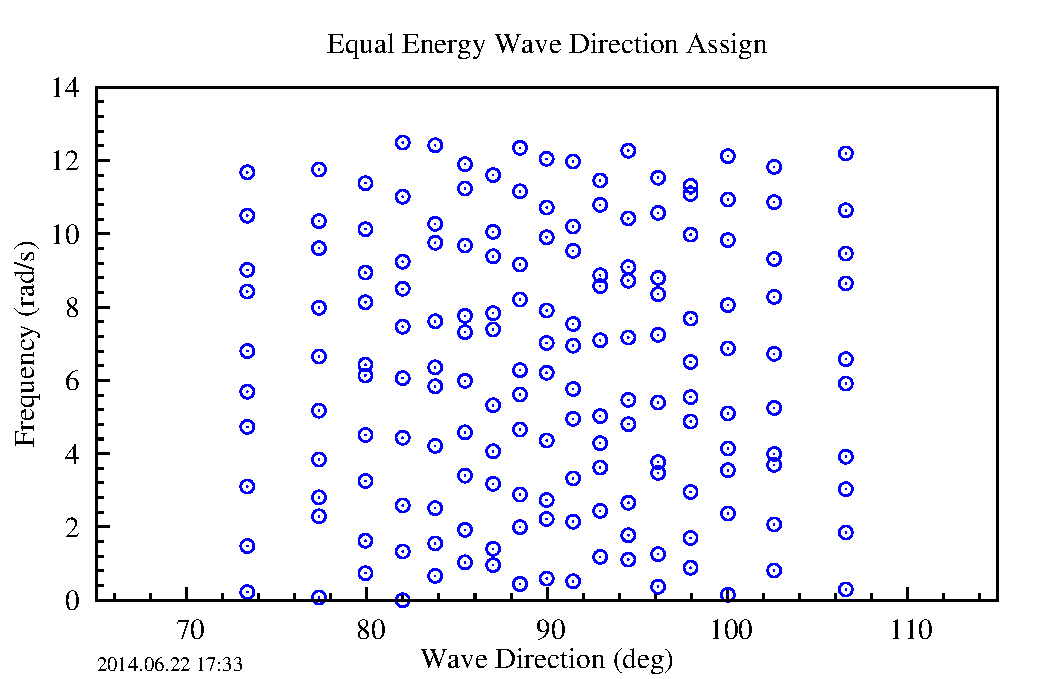
\includegraphics[width=.47\linewidth]{chaps/figures/WaveDirTest/WavesTest_005--wavedir_assign.pdf}
   \caption{Test case 005.  The right plot shows the randomly selected directions for each frequency.\label{fig:MultiDir:WavesTest005}}
\end{figure}

\begin{figure}
   \centering
   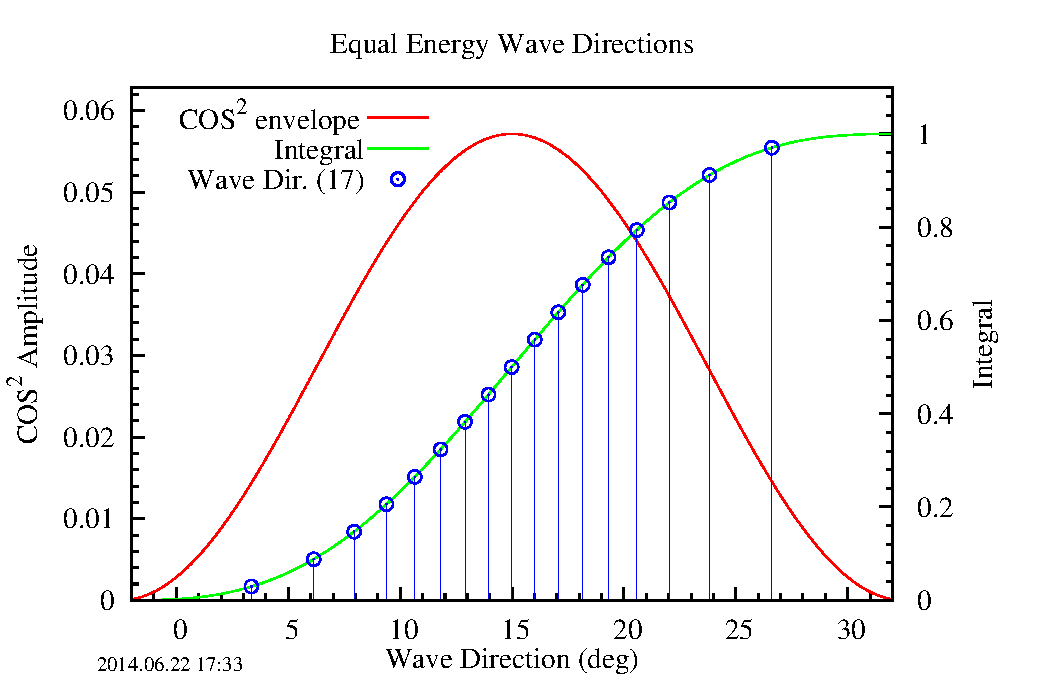
\includegraphics[width=.47\linewidth]{chaps/figures/WaveDirTest/WavesTest_008--equal_energy_disc.pdf}
   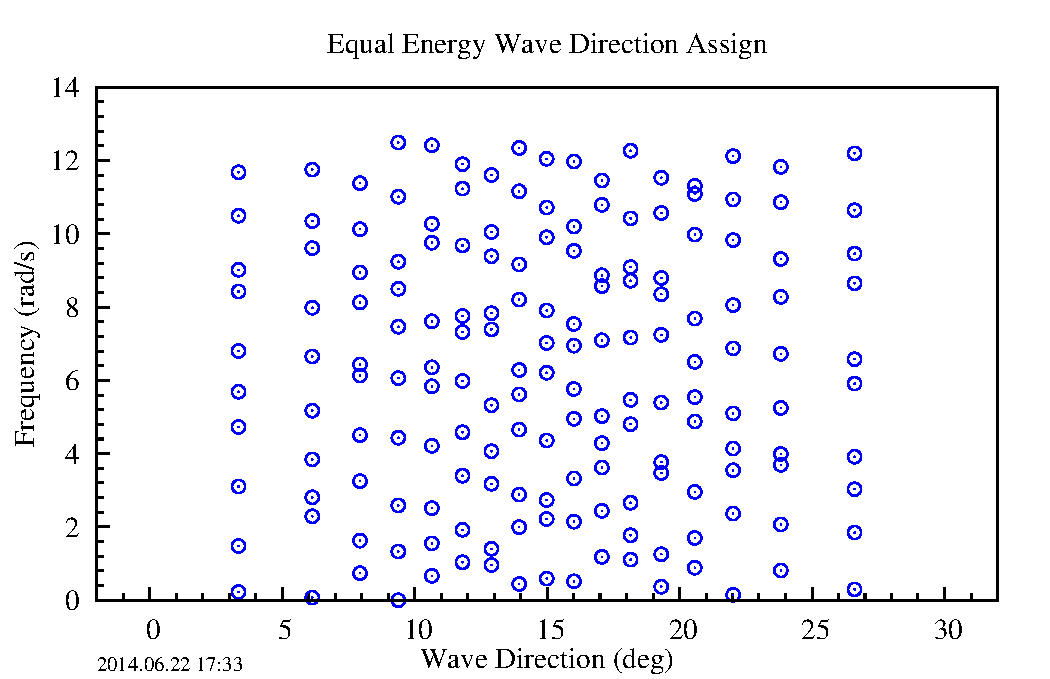
\includegraphics[width=.47\linewidth]{chaps/figures/WaveDirTest/WavesTest_008--wavedir_assign.pdf}
   \caption{Test case 008.  The right plot shows the randomly selected directions for each frequency.\label{fig:MultiDir:WavesTest008}}
\end{figure}



%\section{Modifications to wave velocity and acceleration equations}
%\label{sec:MultiDir:eqMods}
%
%Several of the equations used within the \modname{Waves} module are modified to accomodate the wavedirections as a function of frequency.  In Jason's dissertation, the $cos(\beta)$ and $sin(\beta)$ terms in equation 2-31a, 2-31b, 2-32a, and 2-32b are moved inside the IFFT.  %In the code, these are now implimented as %page 33 of dissertation 
%\begin{equation}
%v_1(t,X,Y,Z) = 
%\label{eq:MultiDir:WaveVelxi}
%\end{equation}


\clearpage
\section{Changes during implimentation}
\begin{description}
   \item[Waves module:]{\varname{InitOutputType\%WaveDir} will continue to contain the mean wave heading.  A new array \varname{InitOutputType\%WaveDirArr} will contain the direction headings for each wave elevation (same number of elements as \varname{WaveElevCO}).}
   \item[Waves module:]{For calculations of wave height, velocity, and acceleration away from the origin, modifications were made to split the wave into $x$ and $y$ components and calculate each separately (used to be single component along wave direction).}
   \item[Waves module:]{the equations for the wave velocity and acceleration used within the \modname{Waves} module are modified to accomodate the wavedirections as a function of frequency.  In Jason's dissertation, the $cos(\beta)$ and $sin(\beta)$ terms in equation 2-31a, 2-31b, 2-32a, and 2-32b are moved inside the IFFT.}  %In the code, these are now implimented as %page 33 of dissertation}
   \item[WAMIT module:]{Change wording about \varname{WaveDir} to correspond to the mean wave direction.  Add in a new variable \varname{WaveDirArr} to handle the directions for each frequency.}
   \item[WAMIT module:]{Change the code to use \varname{WaveDirArr} at each frequency.  This involved combining what had been two one-dimensional interpolations into a single two-dimensional interpolation scheme.}
\end{description}

In addition to the above changes, a new pair of input and output arrays were specified to allow for the calculation of the wave elevation at arbitrarily specified (X,Y) coordinates.  The input array, \varname{WaveElevXY}, of size $2\times N$ allows the for a set of $N$ arbitrary number of $(x,y)$ coordinates to be specified.  For this array, index 1 corresponds to specifies which coordinate ($x$ or $y$) and index 2 corresponds to point number.  If \varname{WaveElevXY} has been allocated at the gluecode or driver level, an array, \varname{WaveElevSeries}, of size \varname{NStepWave}$\times N$ is returned.  The first index of this array is the timestep (of the \varname{NStepWave} timesteps in the simulation), and the second index corresponds to the point number (of $N$ points) specified in the \varname{WaveElevXY} input array.  This has been implimented both within the \modname{Waves} module and within \HD itself.  It has been tested with the \HD driver and with the \modname{WAMIT2} driver code to generate sea surface movies corresponding to each of the 8 tests listed in \Cref{tab:MultiDir:Tests}.


   %\part{Second Order Force Calculations}
\chapter{WAMIT: Output Files}
\label{chap:WamitOutput}


\begin{table}[H]
   \centering
   \caption[Notation for WAMIT output files]{Notation for data contained in the WAMIT output files.  Here $\bar{F}$ is the force quadratic transfer function. The units listed are those given within the WAMIT manual\cite{WAMIT}. Note: some variable names appear differently here than in the WAMIT manual.\label{tab:WamitOutputUnits}}
   \begin{tabular}{cll}
      \toprule
         Variable                   &  Type                       &  Units             \\
      \midrule
         $\tau$                     &  Wave period                &  Seconds           \\
         $\beta$                    &  Wave direction             &  Degrees           \\
         $k$                        &  Force component            &  None              \\
         $\left|\bar{F}\right|$     &  Force QTF Magnitude        &  Nondimensional    \\
         $\theta$                   &  Force QTF Phase            &  Degrees           \\
         $\Re(\bar{F})$             &  Force QTF Real part        &  Nondimensional    \\
         $\Im (\bar{F})$            &  Force QTF Imaginary part   &  Nondimensional    \\     
%         $\rho$                     &  Density of fluid           &  kg/m$^3$          \\
%         $g$                        &  Gravitational constant     &  m/s$^2$           \\
%         $L$                        &  Characteristic length      &  m                 \\
      \bottomrule
   \end{tabular}
\end{table}





WAMIT can use several methods to calculate the normalized second order wave force.  Each of those methods produces a different type of output file.  The calculation methods available to the WAMIT2 module are limited by the WAMIT output files that are available.  \Cref{tab:Wamit2MethodsByFileType} shows what second order force calculation methods are available depending on the WAMIT files available\cite{WAMIT}.
\Cref{tab:WamitOutputUnits} lists the variables used in this document to refer to the various WAMIT outputs.  Note that the notation here differs with the notation used in the WAMIT manual and in Tiago's writings\cite{duarte:2014,WAMIT}.

\section{WAMIT Output}
\Cref{tab:WamitOutputFormat} lists the format for each of the WAMIT output files.
Within these files, the angles and frequencies do not need to be evenly spaced.  Also, it should also be noted that the discretization between $\omega_1$ and $\omega_2$ are not necessarily the same.  This also applies to the angles $\beta_1$ and $\beta_2$.

A value for the period $\tau = 0$ in the WAMIT output file means that the frequency $\omega = \infty$.  A period of $\tau < 0$ is used in the WAMIT output file to indicate $\omega = 0$.

The QTF in the WAMIT output files does not need to be complete since the following relationships are true:
\begin{equation}
   \bar{F}^\text{-}_{mn} = \bar{F}^{\text{-}~*}_{nm}   \qquad \text{and} \qquad   \bar{F}^{+}_{mn} = \bar{F}^{+}_{nm},
\label{eq:WAMIT:QTF_sym}
\end{equation}
where $*$ indicates the complex conjugate.  Note that this implies that the diagonal terms in the second order difference QTF, $\bar{F}^\text{-} (\omega_m,\omega_m) =\bar{F}^{\text{-}~*} (\omega_m,\omega_m)$, are real valued.

The normalized second order wave force in the WAMIT output files is non-dimensional (see Ref~\cite{WAMIT} section 11.6 for details).  These are written as
\begin{equation}
   \bar{F}_k^\text{-}   = \frac{\tilde{F}_k^\text{-}}{\rho g L^a A_m A^*_n} 
         \qquad\text{and}\qquad
   \bar{F}_k^{+}        = \frac{\tilde{F}_k^{+}}{\rho g L^a A_m A_n},
\label{eq:QTF:nondimensional}
\end{equation}
where $a=1$ for forces ($k = 1, 2, 3$) and $a=2$ for moments ($k=4, 5, 6$), $\bar{F}_k$ and $\tilde{F}_k$ are respectively the non-dimensioned and dimensioned QTFs for the $k^\text{th}$ force component, 
and $A_m$ and $A^*_n$ are the complex wave and complex conjugates of the amplitudes. Other variables are listed in \Cref{tab:2ndOrdNotation}.
In order to simplify using the dimensioned wave force in calculations, \Cref{eq:QTF:nondimensional} can be rewritten as
\begin{equation}
    \tilde{F}_k^\text{-}   = A_m A^*_n \left(\bar{F}_k^\text{-}   \rho g L^a\right)    = A_m A^*_n  {F}_k^\text{-} 
         \qquad\text{and}\qquad
     \tilde{F}_k^+         = A_m A_n   \left(\bar{F}_k^+          \rho g L^a\right)    = A_m A_n    {F}_k^+,
\label{eq:QTF:dimensional}
\end{equation}
where ${F}_k^\pm$ is partially dimensioned by $\rho g L^a$, but does not include the wave amplitudes.


\newcommand{\pboxl}[1]{\footnotesize{\parbox[c]{1.35in}{#1}}}
\begin{table}
   \centering
   \caption[Format of WAMIT output files]{WAMIT output files and format (version 6.4/6.1s)\cite{WAMIT}. In this table, $\tau$ is the period of the wave, $\beta_m$ and $\beta_n$ are the wave directions.  The second order complex force term is given by both the amplitude and phase pair ($\left|\bar{F}_m\right|$ and  $\theta_m$), and in terms of its real and imaginary parts ($\Re (\bar{F}_m)$ and $\Im (\bar{F}_m)$).  The index $k$ indicates the force ($k=1\ldots3$) or moment ($k=4\ldots6$) load components.  The indices $m$ and $n$ correspond to the period of the waves that are interacting (see pages 4-9 and 11-13 of Ref.~\citen{WAMIT}).\label{tab:WamitOutputFormat}}
   \tabcolsep=1.75mm
   \begin{tabular}{c>{\raggedright}p{1.35in}ccccccccc}
      \toprule
 File Ext.  &  Description    &  \multicolumn{9}{l}{Output Format} \\
%         File  &                 & \multicolumn{2}{c}{Period}  & \multicolumn{2}{c}{Angle}            & DOF & Ampl.  & Phase  & Real   & Imag.  \\
%         Ext.  &  Description    & \multicolumn{2}{c}{(s)} & \multicolumn{2}{c}{(deg)} & (-) & (-)    & (rad?) & (-)    & (-)    \\
      \midrule
   .7       &  {\pboxl{Mean drift based on momentum flux (WAMIT v. 7 only)}}
            &  $\tau_m$ &                          &  $\beta_{m(1)}$    &  $\beta_{m(2)}$                &  $k$   
            &  $\left|\bar{F}^{-}_{mm}\right|$     &  $\theta_{mm}$     &  $\Re (\bar{F}^{-}_{mm})$      &  $\Im (\bar{F}^{-}_{mm})$      \\[7pt]
   .8       &  {\pboxl{Mean drift (modes 1, 2, and 6)}}
            &  $\tau_m$ &                          &  $\beta_{m(1)}$    &  $\beta_{m(2)}$                &  $k$   
            &  $\left|\bar{F}^{-}_{mm}\right|$     &  $\theta_{mm}$     &  $\Re (\bar{F}^{-}_{mm})$      &  $\Im (\bar{F}^{-}_{mm})$      \\[5pt]
   .9       &  {\pboxl{Mean drift (all modes)}}
            &  $\tau_m$ &                          &  $\beta_{m(1)}$    &  $\beta_{m(2)}$                &  $k$   
            &  $\left|\bar{F}^{-}_{mm}\right|$     &  $\theta_{mm}$     &  $\Re (\bar{F}^{-}_{mm})$      &  $\Im (\bar{F}^{-}_{mm})$      \\[1pt] \midrule
   .10s     &  {\pboxl{Quadratic \nth{2}-order sum forces}}
            &  $\tau_m$ &  $\tau_n$                &  $\beta_{m}$       &  $\beta_n$                     &  $k$   
            &  $\left|\bar{F}_{mn}^{+}\right|$     &  $\theta_{mn}^{+}$ &  $\Re (\bar{F}_{mn}^{+})$      &  $\Im (\bar{F}_{mn}^{+})$      \\[5pt]
   .10d     &  {\pboxl{Quadratic \nth{2}-order difference forces}}
            &  $\tau_m$ &  $\tau_n$                &  $\beta_{m}$       &  $\beta_n$                     &  $k$   
            &  $\left|\bar{F}_{mn}^{-}\right|$     &  $\theta_{mn}^{-}$ &  $\Re (\bar{F}_{mn}^{-})$      &  $\Im (\bar{F}_{mn}^{-})$      \\[5pt]
   .11s     &  {\pboxl{Total \nth{2}-order forces by indirect method (sum)}}
            &  $\tau_m$ &  $\tau_n$                &  $\beta_{m}$       &  $\beta_n$                     &  $k$   
            &  $\left|\bar{F}_{mn}^{+}\right|$     &  $\theta_{mn}^{+}$ &  $\Re (\bar{F}_{mn}^{+})$      &  $\Im (\bar{F}_{mn}^{+})$      \\[7pt]
   .11d     &  {\pboxl{Total \nth{2}-order forces by indirect method (diff)}}
            &  $\tau_m$ &  $\tau_n$                &  $\beta_{m}$       &  $\beta_n$                     &  $k$   
            &  $\left|\bar{F}_{mn}^{-}\right|$     &  $\theta_{mn}^{-}$ &  $\Re (\bar{F}_{mn}^{-})$      &  $\Im (\bar{F}_{mn}^{-})$      \\[7pt]
   .12s     &  {\pboxl{Total \nth{2}-order forces by direct method (sum)}}
            &  $\tau_m$ &  $\tau_n$                &  $\beta_{m}$       &  $\beta_n$                     &  $k$   
            &  $\left|\bar{F}_{mn}^{+}\right|$     &  $\theta_{mn}^{+}$ &  $\Re (\bar{F}_{mn}^{+})$      &  $\Im (\bar{F}_{mn}^{+})$      \\[7pt]
   .12d     &  {\pboxl{Total \nth{2}-order forces by direct method (diff)}}
            &  $\tau_m$ &  $\tau_n$                &  $\beta_{m}$       &  $\beta_n$                     &  $k$   
            &  $\left|\bar{F}_{mn}^{-}\right|$     &  $\theta_{mn}^{-}$ &  $\Re (\bar{F}_{mn}^{-})$      &  $\Im (\bar{F}_{mn}^{-})$      \\
      \bottomrule
   \end{tabular}
\end{table}






\section{Reading WAMIT Data Files}
\label{sec:WamitOuput:Read}
\todo[inline]{Make pretty version of \Cref{fig:2ndOrdRead}}

\subsection{First order WAMIT output files (.3)}
The algorithm used in reading in the first order WAMIT data files involves scanning through the data file multiple times.  This is roughly summarized as:
\begin{enumerate}
   \item{Get wave period information}
   \begin{enumerate}
      \item{Read through file to find the number of wave periods}
      \item{Allocate array to hold the wave periods in the order they appear in the file (\varname{WAMITPer} and \varname{WAMITFreq})}
      \item{Allocate array \varname{SortFreqInd} to hold the ordered indices of the sorted frequencies}
      \item{Allocate array \varname{HdroFreq} to hold the sorted frequencies}
      \item{Read through file to populate the \varname{WAMITPer}, \varname{WAMITFreq} and \varname{SortFreqInd} arrays}
      \item{Read through file and store the sorted frequencies in \varname{HdroFreq}}
   \end{enumerate}
   \item{Get wave directions}
   \begin{enumerate}
      \item{Read through first wave period to get the directions}
      \item{Allocate array to hold the wave directions in the order they appear in the file (\varname{WAMITDir})}
      \item{Allocate array \varname{SortWvDirInd} to hold the ordered indices of the sorted directions}
      \item{Allocate array to hold the ordered indices of the sorted directions (\varname{HdroWvDir})}
      \item{Read through file to populate \varname{WAMITDir} and assemble}
      \item{Read through file and store the sorted directions in \varname{HdroWvDir}}
   \end{enumerate}
   \item{Populate the complex wave information \varname{HdroExctn}}
   \begin{enumerate}
      \item{Read through the file again to populate \varname{HdroExctn}(\varname{SortFreqInd}(K),\varname{SortWvDirInd}(J),I)}
   \end{enumerate}
\end{enumerate}

There are two subtle assumptions about the organization of the WAMIT output file that are made here.  First, the file is always organized such that the wave direction is looped through for each value of the wave period.  The second assumption is that all the force components are grouped for a given wave direction and wave period.  In the case of the second order WAMIT data, this may not be true.

\subsection{Second order WAMIT output files}

The calculations for the second order WAMIT output are very time consuming.  In order to help alleviate this problem, WAMIT allows the user to specify exactly which combinations of wave heading and wave periods to calculate in a .PT2 input file.  As a result, the output file may be very sparse, and may not be ordered in any meaningful way.  Therefore, a different approach that does not make assumptions about the ordering of the file should be used.

\begin{figure}[H]
   \centering
   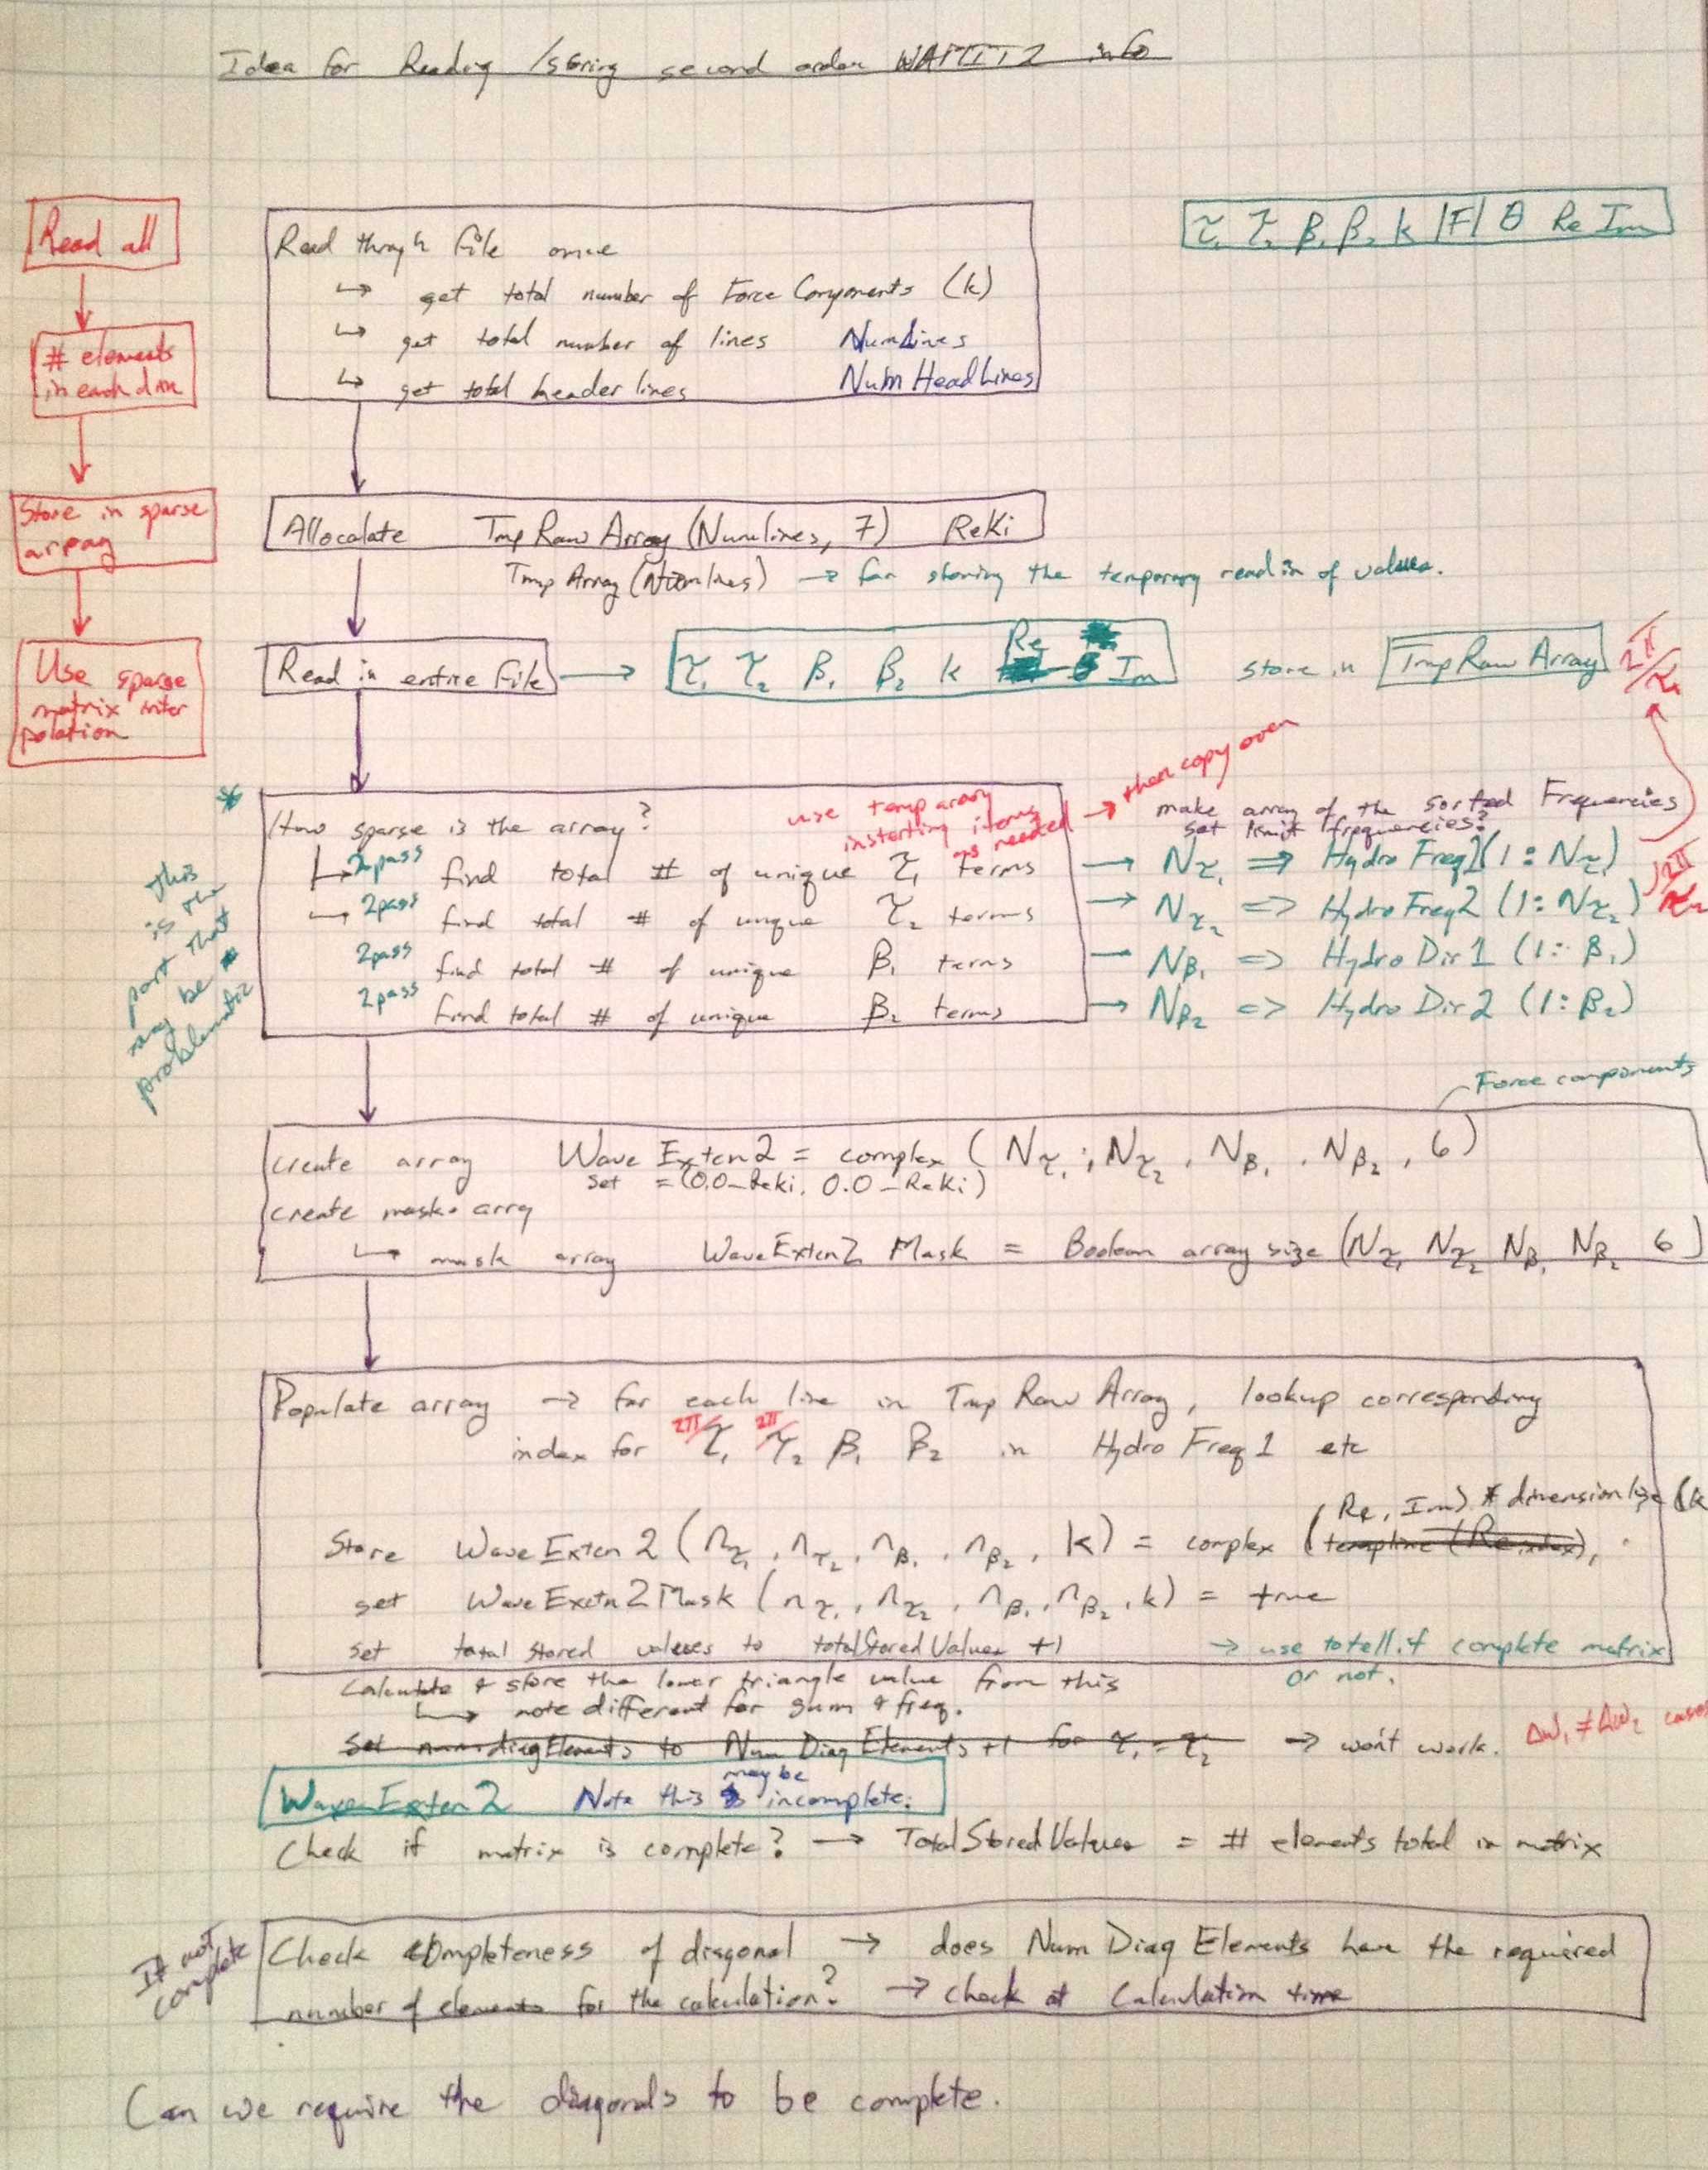
\includegraphics[height=8in]{chaps/figures/WAMIT2--read_Algorithm.jpg}
   \caption{Overview of scheme for reading in 2nd order WAMIT files with two periods (.10, .11, .12).  The algorithm for reading in 2nd order WAMIT files with only one period (.7, .8, .9) should be a simplified version of this algorithm.
      \label{fig:2ndOrdRead}}
\end{figure}

The overall idea of this approach is to read the entire data file a temporary array in memory, and then figure out how many unique values of $\omega_1, \omega_2, \beta_1,$ and $\beta_2$ there are.  Once this has been determined, the arrays storing the sorted frequencies and directions can be allocated along with the array for storing $F^\pm$.  In addition to the array holding the data, a mask array (boolean?) of equal size must be created to store information regarding which values are populated.  This will be necessary for knowing how sparse the array is and for interpolation algorithms that can handle limited sparseness.

Due to the number of times the file would need to be read for this algorithm, it will likely be faster to read everything into memory and then process rather than rewind the file many times (disk IO is slow).  This does impose some memory usage that could be avoided, but given how long it takes WAMIT to perform these calculations, the files are likely to be small (at least in comparison to the wind files).


\clearpage

\section{WAMIT Data Integrity Checks}
\label{sec:WamitOutput:Checks}
A few checks can be enforced to ensure that the calculations within the \modname{WAMIT2} module can be performed using the provided data.  If the limits of frequency or wave direction are set outside what is provided within the WAMIT output data, an error should be issued and the program aborted.  This could be checked during the calculations by checking if either $\omega < \min{(\tilde{\omega})}$ or $\omega > \max{(\tilde{\omega})}$ is true, where $\tilde{\omega}$ is the array of frequencies given in the WAMIT output files.  Alternatively, this could be checked immediately after reading the WAMIT output file by checking against the limits in the \HD input file as follows:
\begin{eqnarray}
   \varname{WvLowCOffD} > \min{(\tilde{\omega}_D)}\\
   \varname{WvHiCOffD}  < \max{(\tilde{\omega}_D)}
\label{eq:WAMIT:DataLimitTest:Diff}
\end{eqnarray}
for difference QTF files, and
\begin{eqnarray}
   \varname{WvLowCOffS} > \min{(\tilde{\omega}_S)}\\
   \varname{WvHiCOffS}  < \max{(\tilde{\omega}_S)}
\label{eq:WAMIT:DataLimitTest:Sum}
\end{eqnarray}
for sum QTF files where $\tilde{\omega}_D$ and $\tilde{\omega}_S$ are the arrays of frequencies found in the difference and sum WAMIT files, respectively.

In addition to checking the frequency range of the WAMIT output files, the wave direction range should also be checked.  The values can be checked agains the \varname{WaveDirMin} and \varname{WaveDirMax} variables (derived from \varname{WaveDir} and \varname{WaveDirRange} in the \HD input file -- see \Cref{chap:MultiDir}).  Care needs to be taken to account for a possible boundary between positive and negative direction headings ($\pi$ and $-\pi$ directions).
%\todo{Expand this to include eqs/pseudocode for checking of WAMIT data files}

%note on the header lines




\endinput
\section{Additional Data Requirements for the WAMIT2 Module}
\label{sec:WamitOutput:Req}

We will add some additional requirements for second order WAMIT files as they become evident (\emph{i.e.} frequency limits).



\begin{table}
\end{table}

\chapter{Second Order Force Calculations}
\label{chap:2ndOrdCalc}

In this chapter, the equations and algorithms used to find the second order hydrodynamic forces from the output of WAMIT are discussed.
The forms of the equations presented here are what is used in the WAMIT2 module within HydroDyn.
  Along with the equations, the methodology and processing necessary to take the WAMIT output file types and parse them for use in the equations is also covered in detail.
The interpolation algorithms used are covered in \Cref{chap:Algorithm}.

\Cref{tab:Wamit2MethodsByFileType} shows which calculations methods can be used depending on what WAMIT output files are available.  The criteria for downselecting information in the file for use in the calculations is given for each method and file type combination.
\begin{table}
   \centering
   \caption[Matrix of possible calculation methods and data file combinations.]
         {Matrix of possible calculation methods and data file combinations.
         The names given in the column marked \emph{Variables} are the independent variables within the file.
         The information used from each file type is given under each method.  Note that for the mean-drift calculation with multi-directional waves,
         only the $\beta_1 = \beta_2$ terms are necessary with the equal-energy approach.  However, if a different multidirectional waves method is used,
         then all the data would be necessary.
      \label{tab:Wamit2MethodsByFileType}}
   \small{
   \begin{tabular}{ccccccc}
      \toprule
         Sea               &  File  &  Independent   &  \multicolumn{4}{c}{Method}                      \\ \cmidrule(lr){4-7}
         Directionality    &  Ext.  &  Variables   & Mean Drift   &  Newman's &  Diff-QTF &  Sum-QTF  \\
      \midrule
         \multirow{6}{*}{\parbox[c]{18mm}{\centering Uni-Directional Seas}}
            &  7  &  \multirow{3}{*}{\parbox[c]{15mm}{\centering $\omega$\\$\beta_1,\beta_2$}}
                  &  \multirow{3}{*}{\parbox[c]{15mm}{\centering $\beta_1 = \beta_2$}}
                     &  \multirow{3}{*}{\parbox[c]{15mm}{\centering $\beta_1 = \beta_2$}}
                        &  \multirow{3}{*}{\parbox[c]{15mm}{\centering Not possible}}
                           &  \multirow{3}{*}{\parbox[c]{15mm}{\centering Not possible}}
                                 \\
            &  8  &  &  &  &  &  \\
            &  9  &  &  &  &  &  \\  \cmidrule(lr){2-7}
            & 10  &  \multirow{3}{*}{\parbox[c]{15mm}{\centering $\omega_1,\omega_2$\\$\beta_1,\beta_2$}}
                  &  \multirow{3}{*}{\parbox[c]{15mm}{\centering $\omega_1=\omega_2$\\$\beta_1=\beta_2$}}
                     &  \multirow{3}{*}{\parbox[c]{15mm}{\centering $\omega_1=\omega_2$\\$\beta_1=\beta_2$}}
                        &  \multirow{3}{*}{\parbox[c]{15mm}{\centering $\beta_1=\beta_2$}}
                           &  \multirow{3}{*}{\parbox[c]{15mm}{\centering $\beta_1=\beta_2$}}
                                 \\
            & 11  &  &  &  &  &  \\
            & 12  &  &  &  &  &  \\
      \midrule
         \multirow{6}{*}{\parbox[c]{18mm}{\centering Multi-Directional Seas}}
            &  7  &  \multirow{3}{*}{\parbox[c]{15mm}{\centering $\omega$\\$\beta_1,\beta_2$}}
                  &  \multirow{3}{*}{\parbox[c]{15mm}{\centering All Data}}   %$\omega_1 = \omega_2$}}
                     &  \multirow{6}{*}{\parbox[c]{15mm}{\centering Not possible}}
                        &  \multirow{3}{*}{\parbox[c]{15mm}{\centering Not possible}}
                           &  \multirow{3}{*}{\parbox[c]{15mm}{\centering Not possible}}
                                 \\
            &  8  &  &  &  &  &  \\
            &  9  &  &  &  &  &  \\ \cmidrule(lr){2-4} \cmidrule(lr){6-7}
            & 10  &  \multirow{3}{*}{\parbox[c]{15mm}{\centering $\omega_1,\omega_2$\\$\beta_1,\beta_2$}}
                  &  \multirow{3}{*}{\parbox[c]{15mm}{\centering $\omega_1=\omega_2$}}
                     &  &  \multirow{3}{*}{\parbox[c]{15mm}{\centering All Data}}
                           &  \multirow{3}{*}{\parbox[c]{15mm}{\centering All Data}}
                                 \\
            & 11  &  &  &  &  &  \\
            & 12  &  &  &  &  &  \\
      \bottomrule
   \end{tabular}
   }
\end{table}




The notation used in this chapter is given in \Cref{tab:2ndOrdNotation} (note that this differs slightly from the notation in the WAMIT manual\cite{WAMIT} and in Tiago's writings\cite{duarte:2014}).
\begin{table}[h!]
   \centering
   \caption{Notation used in the second order force equations.  
            The variable name used in the fortran code is also listed where appropriate.
            \label{tab:2ndOrdNotation}}
   \begin{tabular}{ccl}
      \toprule
         Variable          & Fortran Variable      &  Description                                                       \\
      \midrule
      $A_m$                &                       &  \parbox[t]{3.5in}{Complex amplitude of the $m^\text{th}$ frequency
                                                               given in $Z[m]$ array from the \emph{Waves} module.  This 
                                                               includes a $N/2$ term in it.}                            \\[13pt]
      $a_m$                &                       &  \parbox[t]{3.5in}{Complex amplitude of the $m^\text{th}$ frequency
                                                               given in $Z[m]$ array from the \emph{Waves} module.  This 
                                                               has the $N/2$ term removed.}                             \\[13pt]
      $i$                  & \varname{ImagNmbr}    &  \parbox[t]{3.5in}{The imaginary number $i = \sqrt{-1}$ ($i$ and
                                                               $j$ are not used as indices here to avoid confusion)}    \\[13pt]
      $k$                  &                       &  Index to load component (translation: 1 -- 3; rotation: 4 -- 6)   \\
      $m$                  &                       &  Index to first wave                                               \\
      $n$                  &                       &  Index to second wave                                              \\
      $\mu^\text{-}$       &                       &  Difference index of two waves frequencies ($= m-n$)               \\
      $\mu^{+}$            &                       &  Summation  index of two wave frequencies ($= m+n$)                \\
      $\tau$               & \varname{WAMITPer}    &  Period of wave in WAMIT file                                      \\
      $\tau_1$             & \varname{WAMITPer1}   &  Period of first wave in pair read from WAMIT file                 \\
      $\tau_2$             & \varname{WAMITPer2}   &  Period of second wave in pair read from WAMIT file                \\
      $\omega$             & \varname{Omega}       &  Frequency (rad/s)                                                 \\
      $N$                  & \varname{NStepWave}   &  Total number of timesteps (range 0:N)                             \\
      $N/2$                & \varname{NStepWave2}  &  Total number of positive wave frequencies (range 0:N/2)           \\
      $Z(\omega_m)$        & \varname{WaveElevC0}  &  The discretized complex wave form in the frequency domain         \\
      $\Phi(\omega_m)$     & \varname{WaveDir}     &  Wave direction for each wave frequency                            \\
      $t_\text{max}$       & \varname{WaveTMax}    &  The maximum time of the wave simulation                           \\
      $\Delta t$           & \varname{WaveDT}      &  The timestep for the wave simulation                              \\
      $\omega_\text{lo}$   & \varname{WvLowCOff}   &  The low frequency cutoff for first order waves                    \\
      $\omega_\text{hi}$   & \varname{WvHiCOff}    &  The high frequency cutoff for first order waves                   \\
      $\Delta\omega$       & \varname{WaveDOmega}  &  The frequency stepsize                                            \\
      $\omega_\text{lo-d}$ & \varname{WvLowCOffD}  &  Difference frequency low-cutoff                                   \\
      $\omega_\text{hi-d}$ & \varname{WvHiCOffD}   &  Difference frequency high-cutoff                                  \\
      $\omega_\text{lo-s}$ & \varname{WvLowCOffS}  &  Sum frequency low-cutoff                                          \\
      $\omega_\text{hi-s}$ & \varname{WvHiCOffS}   &  Sum frequency high-cutoff                                         \\
      $\bar{F}^\text{-}_{k}$ &                     &  \parbox[t]{3.5in}{$k^\text{th}$ component of the non-dimensional difference 
                                                                     frequency transfer matrix (data from WAMIT)}       \\[13pt]
      $F^\text{-}_{k}$     &                       &  \parbox[t]{3.5in}{$k^\text{th}$ component of the dimensionalized difference
                                                                     frequency transfer matrix}                         \\[13pt]
      $\bar{F}^\text{+}_{k}$ &                     &  \parbox[t]{3.5in}{$k^\text{th}$ component of the non-dimensional sum 
                                                                     frequency transfer matrix (data from WAMIT)}       \\[13pt]
      $F^\text{+}_{k}$     &                       &  \parbox[t]{3.5in}{$k^\text{th}$ component of the dimensionalized sum
                                                                     frequency transfer matrix}                         \\[13pt]
      $\rho g$             & \varname{RhoXg}       &  Water density * gravity                                           \\
      $L$                  & \varname{WAMITULEN}   &  WAMIT characteristic body length scale                            \\
   \end{tabular}
\end{table}


\section{Overview}
\label{sec:2ndOrdCalc:Overview}

\begin{figure}[ht]
   \begin{center}
      \beginpgfgraphicnamed{General.Flowchart}
         \begin{tikzpicture}

% temporary node for the sectioning labels
\node[tempnode]
      (TmpNode) {};

% WAMIT 1st order
\node[process,right of=TmpNode,node distance=30mm,text width=25mm,text centered] 
      (W1Get) {Read \nth{1}~order WAMIT~output (.7~.8~.9) (\Cref{sec:WamitOuput:Read})};

\node[info,below of=W1Get,node distance=20mm,text width=25mm,text centered]
      (W1Data) {3D matrix\\(possibly sparse)\\$F^\text{-}_k(\omega,\beta_1,\beta_2)$};
   \draw[cl] (W1Get) -- (W1Data);



%WAMIT 2nd
\node[process,right of=W1Get,node distance=60mm,text width=25mm,text centered] 
      (W2Get) {Read \nth{2}~order WAMIT~output (.10d~.11d~.12d) (\Cref{sec:WamitOuput:Read})};

\node[info,below of=W2Get,node distance=20mm,text width=25mm,text centered]
      (W2Data) {4D matrix\\(possibly sparse)\\$F^\pm_k(\omega_1,\omega_2,\beta_1,\beta_2)$};
   \draw[cl] (W2Get) -- (W2Data);

%Equation
\node[anchor=center,process]
      (Equation)  at ($(W1Data)!.5!(W2Data)+(0mm,-55mm)$) {$F^\pm_k(\omega_{m},\omega_{n},\beta_{m},\beta_{n})$};

\draw[red] ($(Equation)+(0mm,0mm)$) ellipse [x radius=17mm, y radius=5mm];

%Solver
\begin{pgfonlayer}{background}
   \filldraw[rounded corners=3mm,draw=blue!30!black!35,
            fill=white!80!blue!20!red!20!black!10]
                        ($(Equation.north west) +(-15mm,34mm)$) coordinate (SolverBoxNW)
            rectangle   ($(Equation.south east)+(5mm,-8mm)$)   coordinate (SolverBoxSE);
   %put box around the equation set
   \draw[rounded corners=1mm,draw=black,thin]
                        ($(Equation.north west) +(-13mm,5mm)$)
            rectangle   ($(Equation.south east)+(2mm,-5mm)$);

   \node[anchor=north west] at ($(SolverBoxNW.north west) +(1mm,-1mm)$) {Solver};
   \node[anchor=east,font=\Huge] (tmp) at ($(Equation.west)+(0mm,0mm)$) {$\sum$};
   \node[anchor=north,font=\scriptsize] at ($(tmp.south)+(0mm,2.3mm)$) {Inner sum};
\end{pgfonlayer}

%Solver inputs
\node[info,text width=15mm,text centered] (SolveInput) at ($(SolverBoxNW |- Equation)+(-20mm,0mm)$) {$Z(\omega)$\\$\Phi(\omega)$\\Limits};
   \draw[cl] (SolveInput) -- ($(SolverBoxNW |- Equation)$);

%Solver results
\node[info,text width=15mm,text centered] (SolveResults) at ($(SolverBoxSE |- Equation)+(20mm,0mm)$) {$F^{\pm (2)}_{\text{ex}~k}$};
   \draw[cl] ($(SolverBoxSE |- Equation)$) -- (SolveResults);



%Interpolation
\node[process,text width=25mm,text centered] (Interpolate) at ($(Equation.north)+(0mm,21mm)$) {3D / 4D Interpolation at each $m$th summation step (\Cref{sec:Algorithm:Interp})};
   \draw[cl] (Interpolate.south) -- ($(Equation)+(0mm,5mm)$);
   \draw[cl] (W1Data) -- (Interpolate);
   \draw[cl] (W2Data) -- (Interpolate);


\end{tikzpicture}
\endinput


%% draw some lines along the side for marking what parts do what
\coordinate (tmp1) at ($(TmpNode |- W1Data)+(0mm,7mm)$);
\coordinate (tmp2) at ($(TmpNode |- W1Info)+(0mm,-5mm)$);
\draw[black]
      ($(tmp1)+(3mm,0mm)$) -- (tmp1) -- (tmp2) 
         node[midway,above,sloped,rotate=180,font=\small] {Data reading} -- +(3mm,0mm);

\coordinate (tmp1) at ($(TmpNode |- W1UniParse)+(0mm,5mm)$);
\coordinate (tmp2) at ($(TmpNode |- W1UniParse)+(0mm,-5mm)$);
\draw[black]
      ($(tmp1)+(3mm,0mm)$) -- (tmp1) -- (tmp2) 
            node[midway,above,sloped,rotate=180,font=\small] {Parsing}-- +(3mm,0mm);

\coordinate (tmp1) at ($(TmpNode |- UniInterp1)+(0mm,5mm)$);
\coordinate (tmp2) at ($(TmpNode |- UniInterp2)+(0mm,-5mm)$);
\draw[black,text width=21mm,text centered]
      ($(tmp1)+(3mm,0mm)$) -- (tmp1) -- (tmp2) 
            node[midway,above,sloped,rotate=180,font=\small] {Interpolation (\Cref{chap:Algorithm})}-- +(3mm,0mm);

   
\end{tikzpicture}
\endinput


      \endpgfgraphicnamed
   \end{center}
\caption{Generalized overview calculation of second order forces.  Here $Z(\omega)$ is the combination complex wave as a function of frequency and $\Phi(\omega)$ is the associated wave direction heading for each frequency.
The 3D and 4D arrays containing the wave force transfer function are interpolated at each step within the innermost summation containing the $F^\pm_k$ terms, or during assembly of the matrix for the FFT.
   \label{fig:General:Flowchart}
}
\end{figure}

In order to simplify the data processing as much as possible, the WAMIT output data will sorted and stored in either a three-dimensional matrix for first order derived transfer matrices (.7, .8, and .9 files), or a four-dimensional for data derived by full QTF methods (.10, .11, and .12 files).  The values needed for each step in the calculation are interpolated from these arrays using either three- or four-dimensional linear interpolation subroutines (see \Cref{chap:Algorithm} for details on the interpolation). The interpolation of $F^\pm_k$ occurs within each step of the summation or during the assembly of the FFT array.  This minimizes the memory storage requirements somewhat.


\clearpage


\section{Frequency range}
\todo[inline]{Add discussion of Nyquist frequency and its effects -- see e-mail and discussion within the code}
The number of timesteps used in the \modname{Waves} module is determined by the total time, $t_\text{max}$, and timestep, $\Delta t$, specified for wave information (\varname{WaveTMax} and \varname{WaveDT} in the \HD input file and code).  The number of timesteps (\varname{NStepWave}) is then set to at least $N \geq  \left(\frac{t_\text{max}}{\Delta t}\right)$ such that $N$ is even and $N/2$ is a product of small numbers (this is advantageous in computing the FFT).
The number of timesteps also limits the number of frequencies present in the wave information to $N/2+1$ frequencies with a maximum frequency of $1/(2 \Delta t)$ in Hz (the Nyquist frequency).
The maximum wave frequency is therefore $\omega_\text{max} = N/2 \cdot \Delta\omega$ where $\omega$ is in radians.
Due to the specifics of the FFT used (see \Cref{sec:Algorithm:FFT}, the number of frequencies stored in the wave information is $N/2+1$ where only positive frequencies are used (values for $\omega < 0$ are derived from the values for $\omega > 0$). 
The full expression for $N$ in can be written as
\begin{equation}
   N = \dfrac{t_\text{max}}{\Delta t} = \dfrac{2 \omega_\text{max}}{\Delta \omega} = \frac{ 2 \pi}{\Delta t \Delta \omega}.
\label{eq:N}
\end{equation}

Three sets of wave frequency cutoffs are applied to the wave conditions.  The first order frequency range is bounded by the limits $\omega_\text{lo}$ and $\omega_\text{hi}$ (set in the \HD input file by \varname{WvLowCOff} and \varname{WvHiCOff}).  These limits are imposed during generation of the wave frequencies in the \modname{Waves} module by setting the amplitudes of $Z(\omega)=0$ for all $\omega$ outside the limits.

The second order wave frequency limits for all three difference methods are given by $\omega_\text{lo-d}$ and $\omega_\text{hi-d}$ (\varname{WvLoCoQTFd} and \varname{WvHiCoQTFd}).
In the case of the mean-drift and Newman's approximation methods where only the diagonal elements (where $\omega_1 = \omega_2$) are considered, the low difference frequency cutoff will likely not have any impact since it will be rare that $\omega_\text{lo-d} > \omega_\text{lo}$ (a warning will be issued if this does occur).\footnote{The mean drift and Newman's approximation will automatically be zeroed for frequencies less than $\omega_\text{lo}$ since they contain $a_m$ terms for each $\omega_m = \omega_m$ diagonal term.}  The high frequency cutoff will likely be set so that $\omega_\text{hi-d} < \omega_\text{hi}$, so this will be important to impose (a warning will be issued if this is not true).

%\todo[inline]{Add warning in code if $\omega_\text{lo-d} > \omega_\text{lo}$ for either mean drift or Newman's.  Did I do this already?}
%\todo[inline]{Add warning in code if $\omega_\text{hi-d} > \omega_\text{hi}$ for either mean drift or Newman's.  Did I do this already?}

The second order wave frequency limits for the full second order QTFs are then set for the difference QTF and sum QTF methods individually.
For the difference QTF method these limits are given by  $\omega_\text{lo-d}$ and $\omega_\text{hi-d}$ (\varname{WvLowCOffD} and \varname{WvHiCOffD}).
For the sum QTF method these limits are given by  $\omega_\text{lo-s}$ and $\omega_\text{hi-s}$ (\varname{WvLowCOffS} and \varname{WvHiCOffS}).
These limits are applied during the summations of the $a_m a_m F(\omega_m,\omega_m)$ and $H_{\mu^\pm}$ terms.

%\missingfigure{add in the figure from p. 145 of notebook}



\section{Wave Amplitude}
\label{sec:2ndOrdCalc:WaveAmp}

The complex wave amplitude in frequency space, $Z(\omega)$, provided by the \modname{Waves} module contains an extra $N/2$ factor on the amplitude.  This factor is not present in the equations given in Ref.~\citen{duarte:2014}.  
The relationship between the amplitude provided by the \modname{Waves} module, $A_m$ and the amplitude used in the paper, $a_m$, is
\begin{equation}
   A_m = \frac{N}{2} a_m.
\label{eq:WaveAmp}
\end{equation}
In the initialization of the \modname{WAMIT2} module, the values stored for the wave elevation from the \modname{Waves} module are divided by $N/2$ before being stored in the \varname{aWaveElevC0} variable.




%%%%%%%%%%%%%%%%%%%%%%%%%%%%%%%%%%%%%%%%%%%%%%%%
%%%%%%%%%%%%%%%%%%%%%%%%%%%%%%%%%%%%%%%%%%%%%%%%
\section{Difference Frequency Force}
\label{sec:2ndOrdCalc:Diff}

There are three methods for calculating the difference frequency force: mean drift, Newman's approximation, and through the full QTF.  Each method has its advantages, and has different data requirements.  In this section, we explore the simplified equations used in the \modname{WAMIT2} module, the data requirements, and the data processing steps for each of the three methods.



%%%%%%%%%%%%%%%%%%%%%%%%%%%%%%%
\subsection{Mean-Drift Method}
\label{sec:2ndOrdCalc:Diff:MeanDrift}
This term arises from the quadratic interactions of the first order problem, and can therefore be calculated without requiring solutions to the second order potential.  This equation is identical to the first part of the difference QTF equation, \Cref{eq:DiffQTF}, where just the diagonal elements of the QTF are used.  This is the simplest of the three difference frequency methods presented here. The single summation equation is given by 
\begin{equation}
   {F_{\text{ex}~k}^{\text{-}(2)}} =
            \Re \left( \sum\limits_{m=1}^{N/2}
                  {a_m} {a_m^*} F_k^\text{-}(\omega_m, \beta_m)\right) \qquad
      \text{for}\quad k=1,2,\ldots,6,
\label{eq:MeanDrift}
\end{equation}
where $k$ indicates the index to the load component,  ${F_{\text{ex}~k}^{\text{-}(2)}}$ is the resulting time independent mean drift force, and $a_m$ and $a_m^*$ are the complex wave amplitude and its complex conjugate for the $m$\textsuperscript{th} frequency.  Note the lack of time dependence in this equation: the mean drift is the average drift force over the entire simulation.
Note that $F_k^\text{-} (\omega_m, \beta_m)$ is the dimensionalized real valued diagonal of the QTF read from the WAMIT file and interpolated for the $m$\textsuperscript{th} wave frequency.  Note that the $\Delta\omega$ term is necessary since this is a numerical integral.
Note also that the summation starts at $m=1$.  The value of $a_0$ is exactly 0, so it does not need to be included.


\begin{figure}[ht]
   \begin{center}
      \beginpgfgraphicnamed{MeanDrift.Flowchart}
         %%% This approach is not correct: we don't want to parse first.  We can do the parsing as part of the loop and interpolate within the loop.
\begin{tikzpicture}

% temporary node for the sectioning labels
\node[tempnode]
      (TmpNode) {};

% WAMIT 1st order
\node[info,right of=TmpNode,node distance=30mm,text width=19mm,text centered] 
      (W1Data) {Read \nth{1}~order WAMIT~output (.7~.8~.9)};

\node[process,below of=W1Data,node distance=13mm]
      (W1Sort) {Sort data};
   \draw[cl] (W1Data) -- (W1Sort);

\node[process,below of=W1Sort,node distance=12mm]
      (W1Convert) {Convert $\tau \rightarrow \omega$};
   \draw[cl] (W1Sort) -- (W1Convert);

\node[info,below of=W1Convert,node distance=12mm]
      (W1Info) {Raw \nth{1} order data};
   \draw[cl] (W1Convert) -- (W1Info);

\node[annotation,right of=W1Info,node distance=25mm,text centered, text width=15mm]
      (W1InfoSize) {$6 \times n_\omega \times n_{\beta_1} \times n_{\beta_2}$};
   \draw[gray] (W1Info) -- (W1InfoSize);

% unidirectional
   \node[process]
         (W1UniParse) at ($(W1Info)+(-13mm,-15mm)$) {$\beta_1=\beta_2$ terms};
      \draw[cl] (W1Info) -- (W1UniParse);
   \node[annotation,text centered, text width=15mm]
         (W1UniParseSize) at ($(W1UniParse)+(-5mm,-8mm)$) {$6 \times n_\omega \times n_{\beta}$};
      \draw[gray] (W1UniParse) -- (W1UniParseSize);
   
% multidirectional
   \node[process] 
         (W1BiParse) at ($(W1Info)+(13mm,-15mm)$)  {all terms};
      \draw[cl] (W1Info) -- (W1BiParse);


%WAMIT 2nd
\node[info,right of=W1Data,node distance=60mm,text width=21mm,text centered] 
      (W2Data) {Read \nth{2}~order WAMIT~output (.10d~.11d~.12d)};

\node[process,below of=W2Data,node distance=13mm]
      (W2Sort) {Sort data};
   \draw[cl] (W2Data) -- (W2Sort);

\node[process,below of=W2Sort,node distance=12mm]
      (W2Convert) {Convert $\tau \rightarrow \omega$};
   \draw[cl] (W2Sort) -- (W2Convert);

\node[info,below of=W2Convert,node distance=12mm]
      (W2Info) {Raw \nth{2} order data};
   \draw[cl] (W2Convert) -- (W2Info);

\node[annotation,right of=W2Info,node distance=27mm,text centered, text width=18mm]
      (W2InfoSize) {$6 \times n_{\omega_1} \times n_{\omega_2} \times n_{\beta_1} \times n_{\beta_2}$};
   \draw[gray] (W2Info) -- (W2InfoSize);

% unidirectional
   \node[process,text width=24mm,text centered]
         (W2UniParse) at ($(W2Info)+(-15mm,-15mm)$) {$\beta_1=\beta_2$ when $\omega_1=\omega_2$ terms};
      \draw[cl] (W2Info) -- (W2UniParse);
   \node[annotation,text centered, text width=15mm]
         (W2UniParseSize) at ($(W2UniParse)+(1mm,-9.5mm)$) {$6 \times n_\omega \times n_{\beta}$};
      \draw[gray] (W2UniParse) -- (W2UniParseSize);
   
% multidir
   \node[process,text width=24mm,text centered]
         (W2BiParse) at ($(W2Info)+(15mm,-15mm)$) {$\omega_1=\omega_2$ terms};
      \draw[cl] (W2Info) -- (W2BiParse);
   \node[annotation,text centered, text width=15mm]
         (W2BiParseSize) at ($(W2BiParse)+(6mm,-10mm)$) {$6 \times n_\omega \times n_{\beta_1} \times n_{\beta_2}$};
      \draw[gray] (W2BiParse) -- (W2BiParseSize);
   


%%%%%%%%%%%%%%%%%%%%%%
% Interpolation step %

% unidirectional
\node[process,anchor=north]
      (UniInterp1) at ($(W1Data)+(5mm,-70mm)$) {Interpolate $\beta$};
   \draw[cl] (W1UniParse) -- (UniInterp1);
   \draw[cl] (W2UniParse) -- (UniInterp1);

\node[process,below of=UniInterp1]
      (UniInterp2) {Interpolate $\omega$};
   \draw[cl] (UniInterp1) -- (UniInterp2);

%set the background box of unidirectional
\begin{pgfonlayer}{background}
\filldraw[rounded corners=3mm,draw=blue!30!black!35,
            fill=white!80!blue!20!red!20!black!10]
      ($(UniInterp1.north west) +(-12mm,2mm)$) 
         rectangle ($(UniInterp2.south east)+(2mm,-2mm)$);
\end{pgfonlayer}
\node[tempnode,anchor=north,font=\footnotesize,text centered,text width=18mm,rotate=90]
      (UniDir) at ($(UniInterp1.west)!.5!(UniInterp2.west)+(-11mm,0mm)$) {\it{Uni-dir waves}\\(2$\times$1D)};



% multidirectional
\coordinate (tmp) at ($(UniInterp1)!.5!(UniInterp2)$);
\node[process,text width=21mm,text centered,anchor=center]
      (BiInterp1) at ($(W2Data |-  tmp) +(-0mm,0mm)$) {Interpolate 3D over $\omega, \beta_1, \beta_2$};
   \draw[red]  (BiInterp1.north west) -- (BiInterp1.south east);
   \draw[red]  (BiInterp1.north east) -- (BiInterp1.south west);
   \draw[cl,gray!50] (W1BiParse) -- (BiInterp1);
   \draw[cl,gray!50] (W2BiParse) -- (BiInterp1);

%set the background box of Multidirectional
\begin{pgfonlayer}{background}
\filldraw[rounded corners=3mm,draw=blue!30!black!35,
            fill=white!80!blue!20!red!20!black!10]
      ($(BiInterp1.north west) +(-12mm,2mm)$) 
         rectangle ($(BiInterp1.south east)+(2mm,-2mm)$);
\end{pgfonlayer}
\node[tempnode,anchor=north,font=\footnotesize,text centered,text width=18mm,rotate=90]
      (MultDir) at ($(BiInterp1.west)+(-11mm,0mm)$) {\it{Multi-dir waves} (\Cref{sec:interp:3d})};



%%%%%%%%%%%%%%%%%%%%%%
% Transfer function
\node[info]
      (TransFunc) at ($(UniInterp1)!.5!(BiInterp1) + (0mm,-25mm)$) {$F^\text{Drift}_k(\omega)$};
   \draw[cl,gray!50] (BiInterp1) -- (TransFunc);
   \draw[cl] (UniInterp2) -- (TransFunc);
\node[annotation,right of=TransFunc,node distance=20mm]
      (TransFuncA) {$6 \times N/2$ terms};
   \draw[gray] (TransFunc) -- (TransFuncA);


% Equation
\node[process,below of=TransFunc]
      (EQ) {\Cref{eq:MeanDrift}};
   \draw[cl] (TransFunc) -- (EQ);



%output
\node[info,below of=EQ,text width=21mm,text centered,node distance=14mm]
      (Output) {Forces and moments to apply to point mesh};
   \draw[cl] (EQ) -- (Output);





%% draw some lines along the side for marking what parts do what
\coordinate (tmp1) at ($(TmpNode |- W1Data)+(0mm,7mm)$);
\coordinate (tmp2) at ($(TmpNode |- W1Info)+(0mm,-5mm)$);
\draw[black]
      ($(tmp1)+(3mm,0mm)$) -- (tmp1) -- (tmp2) 
         node[midway,above,sloped,rotate=180,font=\small] {Data reading} -- +(3mm,0mm);

\coordinate (tmp1) at ($(TmpNode |- W1UniParse)+(0mm,5mm)$);
\coordinate (tmp2) at ($(TmpNode |- W1UniParse)+(0mm,-5mm)$);
\draw[black]
      ($(tmp1)+(3mm,0mm)$) -- (tmp1) -- (tmp2) 
            node[midway,above,sloped,rotate=180,font=\small] {Parsing}-- +(3mm,0mm);

\coordinate (tmp1) at ($(TmpNode |- UniInterp1)+(0mm,5mm)$);
\coordinate (tmp2) at ($(TmpNode |- UniInterp2)+(0mm,-5mm)$);
\draw[black,text width=21mm,text centered]
      ($(tmp1)+(3mm,0mm)$) -- (tmp1) -- (tmp2) 
            node[midway,above,sloped,rotate=180,font=\small] {Interpolation (\Cref{chap:Algorithm})}-- +(3mm,0mm);

   
\end{tikzpicture}
\endinput


      \endpgfgraphicnamed
   \end{center}
\caption{Flow diagram for the mean drift calculation method.  The mean drift equation only involves the diagonal terms where the frequencies $\omega_1 = \omega_2$, and the wave directions $\beta_1 = \beta_2$. 
The WAMIT output files are read in and arranged in either a 3D or 4D array and interpolated at each step in the summation.
See text for how to solve the equation. See \Cref{chap:WamitOutput} for requirements on which WAMIT output files can be used.
   \label{fig:MeanDrift:Flowchart}
}
\end{figure}


\subsubsection*{Solving the Mean-Drift Equations}
\label{sec:2ndOrdCalc:Diff:MeanDrift:solve}
As shown in \Cref{fig:MeanDrift:Flowchart}, the data is stored in either 3D or 4D arrays depending on the file type used.  This is handled by the WAMIT output file reading subroutine, \rname{Read\_DataFiles}, within the \modname{WAMIT2} module.  At each step in the summation of the $m$\textsuperscript{th} term, a call is made to the 3D or 4D interpolation algorithm to find the value of $F^\text{-}_k (\omega_m, \beta_m)$ corresponding to the $Z (\omega_m)$ term in the complex wave amplitude $a_m$.  The limits of $\omega_\text{lo-d} \le \omega_m \le \omega_\text{hi-d}$ are imposed during the summation with values outside this range set to zero.

For multi-directional waves where the equal energy discretization is used, each frequency has a single wave direction associated with it.  Since the mean drift force calculation only involves summing over terms involving only a single frequency at a time, only a single wave direction is involved at each step.  If all the diagonal elements where $\omega_1 = \omega_2$ and $\beta_1 = \beta_2$ were present in the $F^\text{-}_k$ arrays were present, it would be possible to simplify the interpolation required to two dimensional interpolation.  However, since this calculation is performed only at initialization, the calculation penalty for performing a full 3D or 4D interpolation is not as severe as it would be if it were performed at each timestep of the simulation.  Therefore we are choosing to ignore this in favor of simplifying the code implimentation.


%%%%%%%%%%%%%%%%%%%%%%%%%%%%%%%
\clearpage
\subsection{Newman's Approximation Method}
\label{sec:2ndOrdCalc:Diff:Newman}

Newman's original approximation:
\begin{align}
   {F_{\text{ex}~k}^{- (2)}} &\approx 
            \left.   \left[ \Re \left( \sum\limits_{m=1}^{N/2}
                     {a_m} \sqrt{   2 F_k^{-}(\omega_m,\omega_m)}
                     \cdot \mathrm{e}^{\iu \omega_m t} \right) \right]^2 \right|_{F_{k}^{-}(\omega_m,\omega_m) > 0} \nonumber\\
         &-  \left.   \left[ \Re \left( \sum\limits_{m=1}^{N/2}
                     {a_m} \sqrt{  -2 F_k^{-}(\omega_m,\omega_m)}
                     \cdot \mathrm{e}^{\iu \omega_m t} \right) \right]^2 \right|_{F_{k}^{-}(\omega_m,\omega_m) < 0}
      \quad\text{for}\quad k=1,2,\ldots,6,
\label{eq:Newman}
\end{align}
where $k$ indicates the index to the load component, and $a_m$ is the complex wave amplitude for the $m$\textsuperscript{th} frequency.
Note that $F_k^\text{-}$ is the complex valued transfer function read from the WAMIT file and interpolated.  This equation is only valid for uni-directional sea states.

In evaluating the Newman approximation, it must be remembered that the purpose of it is to estimate the off-diagonal ($\omega_1 \ne \omega_2$) values from the diagonal values. If the QTF has large off diagonal components (where $\omega_m \ne \omega_n$), the results will not agree well with the full difference QTF calculations since these elements will be under estimated.

A revised form of Newman's approximation is provided by Standing \emph{et. al.} that is valid for multidirectional sea states.  For multidirectional sea states where each frequency only has on direction assocatied with it, such as with the equal energy discretization, this is equivalent to
\begin{align}
   {F_{\text{ex}~k}^{- (2)}} &\approx 
            \left.   \left| \sum\limits_{m=1}^{N/2}
                     {a_m} \sqrt{   F_k^{-}(\omega_m,\omega_m)}
                     \cdot \mathrm{e}^{\iu \omega_m t} \right|^2 \right|_{F_{k}^{-}(\omega_m,\omega_m) > 0} \nonumber\\
         &-  \left.   \left| \sum\limits_{m=1}^{N/2}
                     {a_m} \sqrt{  -F_k^{-}(\omega_m,\omega_m)}
                     \cdot \mathrm{e}^{\iu \omega_m t} \right|^2 \right|_{F_{k}^{-}(\omega_m,\omega_m) < 0}
      \quad\text{for}\quad k=1,2,\ldots,6,
\label{eq:NewmanRevised}
\end{align}
This equation has been implimented as a Fourier sum rather than IFFT.  It turns out that this implimentation is exactly the same speed as doing the full DiffQTF (within 3\%).


\subsubsection{Mean drift and Newman's approximation}
The mean drift term is already included in the Newman's approximation, so there is no need to add it to the result.  This can be proven by expanding out the squares of the summations and collecting all terms where $m=n$ together.  These collected terms can be written as the mean drift term.  For this proof, it is helpful to remember that for a a given complex value, $C=a+\iu b$, we can write:
\begin{equation}
   \left(\left| C \right| \right)^2 = \left( \sqrt{a^2 + b^2} \right)^2 = a^2 + b^2 = ( a +\iu b ) ( a -\iu b ) = C\cdot C^*
\label{eq:absComplexSquared}
\end{equation}
where $C^*$ is the complex conjugate of $C$.

Taking \Cref{eq:NewmanRevised} and expanding out the terms using \Cref{eq:absComplexSquared}
\begin{align}
   {F_{\text{ex}~k}^{- (2)}} &\approx 
            \left.   \left( \sum\limits_{m=1}^{N/2}
                        {a_m} \sqrt{   F_k^{-}(\omega_m,\omega_m)}
                        \cdot \mathrm{e}^{\iu \omega_m t} \right)
                     \left( \sum\limits_{m=1}^{N/2}
                        {a_m^*} \sqrt{   F_k^{-~*}(\omega_m,\omega_m)}
                        \cdot \mathrm{e}^{- \iu \omega_m t} \right)
              \right|_{F_{k}^{-}(\omega_m,\omega_m) > 0} \nonumber\\
         &-  \left.  \left( \sum\limits_{m=1}^{N/2}
                        {a_m} \sqrt{  -F_k^{-}(\omega_m,\omega_m)}
                        \cdot \mathrm{e}^{\iu \omega_m t} \right)
                     \left( \sum\limits_{m=1}^{N/2}
                        {a_m^*} \sqrt{  -F_k^{-~*}(\omega_m,\omega_m)}
                        \cdot \mathrm{e}^{- \iu \omega_m t} \right)
              \right|_{F_{k}^{-~*}(\omega_m,\omega_m) < 0}.
\label{eq:NewmanRevised2}
\end{align}
Looking at just the first term (${F_{k}^{-}(\omega_m,\omega_m) > 0}$) and remembering that $F_k^{-}(\omega_m,\omega_m) = F_k^{-~*}(\omega_m,\omega_m)$, we can expand all the crossmultiplied terms, collect the terms where $m=n$, and group the other terms where $m \ne n$.  This yields for the first term
\begin{align}
   \text{Term 1} &=  {a_1}{a_1^*} F_k^{-}(\omega_1,\omega_1) \mathrm{e}^{\iu (\omega_1 - \omega_1) t} +
                     {a_2}{a_2^*} F_k^{-}(\omega_2,\omega_2) \mathrm{e}^{\iu (\omega_2 - \omega_2) t} + \ldots \nonumber\\
                 &+  {a_{N/2}}{a_{N/2}^*} F_k^{-}(\omega_{N/2},\omega_{N/2}) \mathrm{e}^{\iu (\omega_{N/2} - \omega_{n/2}) t} \nonumber\\
                 &+  O_{m \ne n}\left(
                        \left(\sum\limits_{m=1}^{N/2}
                        {a_m} \sqrt{   F_k^{-}(\omega_m,\omega_m)}
                        \cdot \mathrm{e}^{\iu \omega_m t} \right)
                     \left( \sum\limits_{m=1}^{N/2}
                        {a_m^*} \sqrt{   F_k^{-~*}(\omega_m,\omega_m)}
                        \cdot \mathrm{e}^{- \iu \omega_m t} \right)\right) \nonumber\\
                 &= \sum\limits_{m=1}^{N/2} {a_m} {a_m^*} F_k^{-}(\omega_m,\omega_m) \nonumber\\
                 &+  O_{m \ne n}\left(
                        \left(\sum\limits_{m=1}^{N/2}
                        {a_m} \sqrt{   F_k^{-}(\omega_m,\omega_m)}
                        \cdot \mathrm{e}^{\iu \omega_m t} \right)
                     \left( \sum\limits_{m=1}^{N/2}
                        {a_m^*} \sqrt{   F_k^{-~*}(\omega_m,\omega_m)}
                        \cdot \mathrm{e}^{- \iu \omega_m t} \right)\right).
\label{eq:NewmanRevised2t1}
\end{align}
The second term is very similar to the first term.  Keeping the negative sign with the term, when expanded and multiplied together it yields
\begin{align}
   \text{Term 2} &= - {a_1}{a_1^*} (-F_k^{-}(\omega_1,\omega_1)) \mathrm{e}^{\iu (\omega_1 - \omega_1) t} +
                    - {a_2}{a_2^*} (-F_k^{-}(\omega_2,\omega_2)) \mathrm{e}^{\iu (\omega_2 - \omega_2) t} + \ldots \nonumber\\
                 &- {a_{N/2}}{a_{N/2}^*} (-F_k)^{-}(\omega_{N/2},\omega_{N/2}) \mathrm{e}^{\iu (\omega_{N/2} - \omega_{n/2}) t} \nonumber\\
                 &-  O_{m \ne n}\left(
                        \left(\sum\limits_{m=1}^{N/2}
                        {a_m} \sqrt{ - F_k^{-}(\omega_m,\omega_m)}
                        \cdot \mathrm{e}^{\iu \omega_m t} \right)
                     \left( \sum\limits_{m=1}^{N/2}
                        {a_m^*} \sqrt{ - F_k^{-~*}(\omega_m,\omega_m)}
                        \cdot \mathrm{e}^{- \iu \omega_m t} \right)\right) \nonumber\\
                 &= \sum\limits_{m=1}^{N/2} {a_m} {a_m^*} F_k^{-}(\omega_m,\omega_m) \nonumber\\
                 &+  O_{m \ne n}\left(
                        \left(\sum\limits_{m=1}^{N/2}
                        {a_m} \sqrt{ - F_k^{-}(\omega_m,\omega_m)}
                        \cdot \mathrm{e}^{\iu \omega_m t} \right)
                     \left( \sum\limits_{m=1}^{N/2}
                        {a_m^*} \sqrt{ - F_k^{-~*}(\omega_m,\omega_m)}
                        \cdot \mathrm{e}^{- \iu \omega_m t} \right)\right).
\label{eq:NewmanRevised2t2}
\end{align}
Combining the first terms from \Cref{eq:NewmanRevised2t1} and \Cref{eq:NewmanRevised2t2} where the first one contains all positive $F^-$ terms and the second contains all negative $F^-$ terms, we arrive at the equation for the mean drift given in \Cref{eq:MeanDrift}
\begin{equation}
        \left. \sum\limits_{m=1}^{N/2} {a_m} {a_m^*} F_k^{-}(\omega_m,\omega_m)\right|_{F_{k}^{-~*}(\omega_m,\omega_m) > 0}
      + \left. \sum\limits_{m=1}^{N/2} {a_m} {a_m^*} F_k^{-}(\omega_m,\omega_m)\right|_{F_{k}^{-~*}(\omega_m,\omega_m) < 0}
      =        \sum\limits_{m=1}^{N/2} {a_m} {a_m^*} F_k^{-}(\omega_m,\omega_m).
\label{eq:NewmanMnDrift}
\end{equation}

\subsubsection{Standing's equation}
Starting with \Cref{eq:NewmanRevised2}, we can substitute in for the $-F_k^- = \left| F_k^- \right|$ within the square root for when $F_{k}^{-~*}(\omega_m,\omega_m) < 0$ and $F_k^- = \left| F_k^- \right|$ within the square root for when $F_{k}^{-~*}(\omega_m,\omega_m) > 0$ to yield
\begin{align}
   {F_{\text{ex}~k}^{- (2)}} &\approx 
            \left.   \left( \sum\limits_{m=1}^{N/2}
                        {a_m}    \sqrt{  \left| F_k^{-}(\omega_m,\omega_m)    \right|}
                        \cdot \mathrm{e}^{\iu \omega_m t} \right)
                     \left( \sum\limits_{m=1}^{N/2}
                        {a_m^*}  \sqrt{  \left| F_k^{-}(\omega_m,\omega_m)    \right|}
                        \cdot \mathrm{e}^{- \iu \omega_m t} \right)
              \right|_{F_{k}^{-}(\omega_m,\omega_m) > 0} \nonumber\\
         &-  \left.  \left( \sum\limits_{m=1}^{N/2}
                        {a_m}    \sqrt{  \left| F_k^{-}(\omega_m,\omega_m)    \right|}
                        \cdot \mathrm{e}^{\iu \omega_m t} \right)
                     \left( \sum\limits_{m=1}^{N/2}
                        {a_m^*}  \sqrt{  \left| F_k^{-}(\omega_m,\omega_m)    \right|}
                        \cdot \mathrm{e}^{- \iu \omega_m t} \right)
              \right|_{F_{k}^{-~*}(\omega_m,\omega_m) < 0}.
\label{eq:NewmanRevised3}
\end{align}
Now that $F_k^-$ is treated in such a way that the sign of it is not kept within the square root, we can collect the first and second term together in \Cref{eq:NewmanRevised3} by introducing the $\mathrm{sgn}$ function as
\begin{align}
   {F_{\text{ex}~k}^{- (2)}} &\approx 
            \left.   \left( \sum\limits_{m=1}^{N/2} \mathrm{sgn}\left(F_k^-\right)
                        {a_m}    \sqrt{  \left| F_k^{-}(\omega_m,\omega_m)    \right|}
                        \cdot \mathrm{e}^{\iu \omega_m t} \right)
                     \left( \sum\limits_{m=1}^{N/2}
                        {a_m^*}  \sqrt{  \left| F_k^{-}(\omega_m,\omega_m)    \right|}
                        \cdot \mathrm{e}^{- \iu \omega_m t} \right)
              \right|_{F_{k}^{-}(\omega_m,\omega_m) > 0}    \nonumber\\
         &+ \left.  \left( \sum\limits_{m=1}^{N/2} \mathrm{sgn}\left(F_k^-\right)
                        {a_m}    \sqrt{  \left| F_k^{-}(\omega_m,\omega_m)    \right|}
                        \cdot \mathrm{e}^{\iu \omega_m t} \right)
                     \left( \sum\limits_{m=1}^{N/2}
                        {a_m^*}  \sqrt{  \left| F_k^{-}(\omega_m,\omega_m)    \right|}
                        \cdot \mathrm{e}^{- \iu \omega_m t} \right)
              \right|_{F_{k}^{-~*}(\omega_m,\omega_m) < 0}  \nonumber\\
         &=          \left( \sum\limits_{m=1}^{N/2} \mathrm{sgn}\left(F_k^-\right)
                        {a_m}    \sqrt{  \left| F_k^{-}(\omega_m,\omega_m)    \right|}
                        \cdot \mathrm{e}^{\iu \omega_m t} \right)
                     \left( \sum\limits_{m=1}^{N/2}
                        {a_m^*}  \sqrt{  \left| F_k^{-}(\omega_m,\omega_m)    \right|}
                        \cdot \mathrm{e}^{- \iu \omega_m t} \right)\nonumber\\
         &=          \left( \sum\limits_{m=1}^{N/2} \mathrm{sgn}\left(F_k^-\right)
                        \widetilde{a_m}    \sqrt{  \left| F_k^{-}(\omega_m,\omega_m)    \right|}
                        \cdot \mathrm{e}^{\iu \omega_m t - \phi_m} \right)
                     \left( \sum\limits_{m=1}^{N/2}
                        \widetilde{a_m}  \sqrt{  \left| F_k^{-}(\omega_m,\omega_m)    \right|}
                        \cdot \mathrm{e}^{- \iu \omega_m t + \phi_m} \right)
\label{eq:NewmanRevised4}
\end{align}
which is Standings version of the equation with $\widetilde{a_m} ~ e^{- \phi_m} = a_m$ (Standing carries the phase term of the wave amplitude within the exponential).


%\todo[inline]{add algorithm figure -- page 151 in notebook}

%\begin{figure}[ht]
%   \begin{center}
%      \beginpgfgraphicnamed{Newman.Flowchart}
%         \begin{tikzpicture}

% temporary node for the sectioning labels
\node[tempnode]
      (TmpNode) {};

% WAMIT 1st order
\node[process,right of=TmpNode,node distance=30mm,text width=25mm,text centered] 
      (W1Get) {Read \nth{1}~order WAMIT~output (.7~.8~.9) (\Cref{sec:WamitOuput:Read})};

\node[info,below of=W1Get,node distance=20mm,text width=25mm,text centered]
      (W1Data) {3D matrix\\(possibly sparse)\\$F^\text{-}_k(\omega,\beta_1,\beta_2)$};
   \draw[cl] (W1Get) -- (W1Data);



%WAMIT 2nd
\node[process,right of=W1Get,node distance=60mm,text width=25mm,text centered] 
      (W2Get) {Read \nth{2}~order WAMIT~output (.10d~.11d~.12d) (\Cref{sec:WamitOuput:Read})};

\node[info,below of=W2Get,node distance=20mm,text width=25mm,text centered]
      (W2Data) {4D matrix\\(possibly sparse)\\$F^\text{-}_k(\omega_1,\omega_2,\beta_1,\beta_2)$};
   \draw[cl] (W2Get) -- (W2Data);

%Equation
\node[anchor=center,process]
      (Equation)  at ($(W1Data)!.5!(W2Data)+(0mm,-55mm)$) {$A_m A^*_m ~ F^\text{-}_k(\omega_{m},\omega_{m},\beta_{m},\beta_{m})$};

\draw[red] ($(Equation)+(6mm,0mm)$) ellipse [x radius=17mm, y radius=5mm];

%Solver
\begin{pgfonlayer}{background}
   \filldraw[rounded corners=3mm,draw=blue!30!black!35,
            fill=white!80!blue!20!red!20!black!10]
                        ($(Equation.north west) +(-15mm,34mm)$) coordinate (SolverBoxNW)
            rectangle   ($(Equation.south east)+(5mm,-8mm)$)   coordinate (SolverBoxSE);
   %put box around the equation set
   \draw[rounded corners=1mm,draw=black,thin]
                        ($(Equation.north west) +(-13mm,5mm)$)
            rectangle   ($(Equation.south east)+(2mm,-5mm)$);

   \node[anchor=north west] at ($(SolverBoxNW.north west) +(1mm,-1mm)$) {Solver};
   \node[anchor=east,font=\Huge] (tmp) at ($(Equation.west)+(0mm,0mm)$) {$\sum$};
   \node[anchor=north,font=\footnotesize] at ($(tmp.south)+(0mm,2.0mm)$) {$m_{\omega_\text{lo-d}}$};
   \node[anchor=south,font=\footnotesize] at ($(tmp.north)+(0mm,-2.0mm)$) {$m_{\omega_\text{hi-d}}$};
\end{pgfonlayer}

%Solver inputs
\node[info,text width=15mm,text centered] (SolveInput) at ($(SolverBoxNW |- Equation)+(-20mm,0mm)$) {$Z(\omega,\beta)$\\Limits};
   \draw[cl] (SolveInput) -- ($(SolverBoxNW |- Equation)$);

%Solver results
\node[info,text width=15mm,text centered] (SolveResults) at ($(SolverBoxSE |- Equation)+(20mm,0mm)$) {$F^{\text{-} (2)}_{\text{ex}~k}$};
   \draw[cl] ($(SolverBoxSE |- Equation)$) -- (SolveResults);



%Interpolation
\node[process,text width=25mm,text centered] (Interpolate) at ($(Equation.north)+(0mm,21mm)$) {3D / 4D Interpolation at each $m$th summation step (\Cref{sec:Algorithm:Interp})};
   \draw[cl] (Interpolate.south) -- ($(Equation)+(4mm,5mm)$);
   \draw[cl] (W1Data) -- (Interpolate);
   \draw[cl] (W2Data) -- (Interpolate);


\end{tikzpicture}
\endinput


%% draw some lines along the side for marking what parts do what
\coordinate (tmp1) at ($(TmpNode |- W1Data)+(0mm,7mm)$);
\coordinate (tmp2) at ($(TmpNode |- W1Info)+(0mm,-5mm)$);
\draw[black]
      ($(tmp1)+(3mm,0mm)$) -- (tmp1) -- (tmp2) 
         node[midway,above,sloped,rotate=180,font=\small] {Data reading} -- +(3mm,0mm);

\coordinate (tmp1) at ($(TmpNode |- W1UniParse)+(0mm,5mm)$);
\coordinate (tmp2) at ($(TmpNode |- W1UniParse)+(0mm,-5mm)$);
\draw[black]
      ($(tmp1)+(3mm,0mm)$) -- (tmp1) -- (tmp2) 
            node[midway,above,sloped,rotate=180,font=\small] {Parsing}-- +(3mm,0mm);

\coordinate (tmp1) at ($(TmpNode |- UniInterp1)+(0mm,5mm)$);
\coordinate (tmp2) at ($(TmpNode |- UniInterp2)+(0mm,-5mm)$);
\draw[black,text width=21mm,text centered]
      ($(tmp1)+(3mm,0mm)$) -- (tmp1) -- (tmp2) 
            node[midway,above,sloped,rotate=180,font=\small] {Interpolation (\Cref{chap:Algorithm})}-- +(3mm,0mm);

   
\end{tikzpicture}
\endinput


%      \endpgfgraphicnamed
%   \end{center}
%\caption{Flow diagram for the Newman's approximation method.  $\tau$ is the period, $\omega$ is the corresponding frequency, and $\beta$ is the wave direction.  The \nth{1} and \nth{2} order {\tt WAMIT} output files are read in and arranged in ascending order within the {\tt WAMIT2\_Init} routine (\Cref{sec:WAMIT2Init}).
%   \label{fig:Newman:Flowchart}
%}
%\end{figure}


%%%%%%%%%%%%%%%%%%%%%%%%%%%%%%%
\clearpage
\subsection{Difference QTF Method}
\label{sec:2ndOrdCalc:Diff:DiffQTF}

\begin{align}
   {F_{\text{ex}~k}^{(-)(2)}} &= \Re 
      \left(
         \sum\limits_{m=1}^{N/2}   a_m a_m^* F_k^{-}(\omega_m,\omega_m) + 
         2 \cdot \sum\limits_{\mu^\text{-}=1}^{N/2-1} H_{\mu^\text{-}} \mathrm{e}^{\iu(\omega_{\mu^\text{-}})t}
      \right)  ,\quad&\text{for}\quad k=1,2,\ldots,6 \label{eq:DiffQTF}\\
   &\text{where}\quad
   H_{\mu^\text{-}} = \dfrac{1}{2} \sum\limits_{n=0}^{N/2-\mu^\text{-}} a_{\mu^\text{-}+n} a_n^* F_k^{-}(\omega_{\mu^\text{-}+n},\omega_n),
      \quad&\text{for}\quad 1\le\mu^\text{-}\le N-1
\label{eq:DiffQTF:H}
\end{align}

In the first term, the summation starts at $m=1$.  The value of $a_0$ is exactly 0, so it does not need to be included.

%\todo[inline]{Add algorithm figure -- p. 153 in notebook}

%\begin{figure}[ht]
%   \begin{center}
%      \beginpgfgraphicnamed{DiffQTF.Flowchart}
%         \begin{tikzpicture}

% temporary node for the sectioning labels
\node[tempnode]
      (TmpNode) {};


%WAMIT 2nd
\node[info,right of=TmpNode,node distance=50mm,text width=21mm,text centered] 
      (W2Data) {Read \nth{2}~order WAMIT~output (.10d~.11d~.12d)};

\node[process,below of=W2Data,node distance=13mm]
      (W2Sort) {Sort data};
   \draw[cl] (W2Data) -- (W2Sort);

\node[process,below of=W2Sort,node distance=12mm]
      (W2Convert) {Convert $\tau \rightarrow \omega$};
   \draw[cl] (W2Sort) -- (W2Convert);

\node[info,below of=W2Convert,node distance=12mm]
      (W2Info) {Raw \nth{2} order data};
   \draw[cl] (W2Convert) -- (W2Info);

% unidirectional
   \node[process,text width=24mm,text centered]
         (W2UniParse) at ($(W2Info)+(-15mm,-15mm)$) {$\beta_1=\beta_2$ terms};
      \draw[cl] (W2Info) -- (W2UniParse);
   
% multidir
   \node[process,text width=24mm,text centered]
         (W2BiParse) at ($(W2Info)+(15mm,-15mm)$) {Full QTF};
      \draw[cl] (W2Info) -- (W2BiParse);


%%%%%%%%%%%%%%%%%%%%%%
% Interpolation step %

% unidirectional
\node[process,anchor=north]
      (UniInterp1) at ($(W2Data)+(-20mm,-65mm)$) {Interpolate $\beta$};
   \draw[cl] (W2UniParse) -- (UniInterp1);

\node[process,below of=UniInterp1]
      (UniInterp2) {Interpolate $\omega_1, \omega_2$};
   \draw[cl] (UniInterp1) -- (UniInterp2);

%set the background box of unidirectional
\begin{pgfonlayer}{background}
\filldraw[rounded corners=3mm,draw=blue!30!black!35,
            fill=white!80!blue!20!red!20!black!10]
      ($(UniInterp1.north west) +(-14mm,2mm)$) 
         rectangle ($(UniInterp2.south east)+(2mm,-2mm)$);
\end{pgfonlayer}
\node[tempnode,anchor=north,font=\footnotesize,text centered,text width=20mm,rotate=90]
      (UniDir) at ($(UniInterp1.west)!.5!(UniInterp2.west)+(-11.5mm,0mm)$) {\it{Uni-dir waves} (\Cref{sec:interp:1d,sec:interp:2d})};



% multidirectional
\coordinate (tmp) at ($(UniInterp1)!.5!(UniInterp2)$);
\node[process,text width=21mm,text centered,anchor=center]
      (BiInterp1) at ($(W2Data |-  tmp) +(25mm,0mm)$) {Interpolate 4D over $\omega_1, \omega_2, \beta_1, \beta_2$};
   \draw[cl] (W2BiParse) -- (BiInterp1);

%set the background box of Multidirectional
\begin{pgfonlayer}{background}
\filldraw[rounded corners=3mm,draw=blue!30!black!35,
            fill=white!80!blue!20!red!20!black!10]
      ($(BiInterp1.north west) +(-12mm,3mm)$) 
         rectangle ($(BiInterp1.south east)+(2mm,-3mm)$);
\end{pgfonlayer}
\node[tempnode,anchor=north,font=\footnotesize,text centered,text width=18mm,rotate=90]
      (MultDir) at ($(BiInterp1.west)+(-11mm,0mm)$) {\it{Multi-dir waves} (\Cref{sec:interp:4d})};



%%%%%%%%%%%%%%%%%%%%%%
% Transfer function
\node[info]
      (TransFunc) at ($(W2Data) + (0mm,-95mm)$) {$F^{-}_k(\omega_m,\omega_n)$};
   \draw[cl] (BiInterp1) -- (TransFunc);
   \draw[cl] (UniInterp2) -- (TransFunc);

% Equation
\node[process,below of=TransFunc]
      (EQ) {\Cref{eq:DiffQTF}};
   \draw[cl] (TransFunc) -- (EQ);



%output
\node[info,below of=EQ,text width=21mm,text centered,node distance=14mm]
      (Output) {Forces and moments to apply to point mesh};
   \draw[cl] (EQ) -- (Output);





%% draw some lines along the side for marking what parts do what
\coordinate (tmp1) at ($(TmpNode |- W2Data)+(0mm,7mm)$);
\coordinate (tmp2) at ($(TmpNode |- W2Info)+(0mm,-5mm)$);
\draw[black]
      ($(tmp1)+(3mm,0mm)$) -- (tmp1) -- (tmp2) 
         node[midway,above,sloped,rotate=180,font=\small] {Data reading} -- +(3mm,0mm);

\coordinate (tmp1) at ($(TmpNode |- W2UniParse)+(0mm,5mm)$);
\coordinate (tmp2) at ($(TmpNode |- W2UniParse)+(0mm,-5mm)$);
\draw[black]
      ($(tmp1)+(3mm,0mm)$) -- (tmp1) -- (tmp2) 
            node[midway,above,sloped,rotate=180,font=\small] {Parsing}-- +(3mm,0mm);

\coordinate (tmp1) at ($(TmpNode |- UniInterp1)+(0mm,5mm)$);
\coordinate (tmp2) at ($(TmpNode |- UniInterp2)+(0mm,-5mm)$);
\draw[black,text width=21mm,text centered]
      ($(tmp1)+(3mm,0mm)$) -- (tmp1) -- (tmp2) 
            node[midway,above,sloped,rotate=180,font=\small] {Interpolation (\Cref{chap:Algorithm})}-- +(3mm,0mm);

   
\end{tikzpicture}
\endinput


%      \endpgfgraphicnamed
%   \end{center}
%\caption{Flow diagram for the full difference QTF method.  $\tau$ is the period, $\omega$ is the corresponding frequency, and $\beta$ is the wave direction.  The \nth{1} and \nth{2} order {\tt WAMIT} output files are read in and arranged in ascending order within the {\tt WAMIT2\_Init} routine (\Cref{sec:WAMIT2Init}).
%   \label{fig:DiffQTF:Flowchart}
%}
%\end{figure}



%%%%%%%%%%%%%%%%%%%%%%%%%%%%%%%%%%%%%%%%%%%%%%%%
%%%%%%%%%%%%%%%%%%%%%%%%%%%%%%%%%%%%%%%%%%%%%%%%
\clearpage
\section{Summation Frequency Force}
\label{sec:2ndOrdCalc:Sum}
There is only one method for calculating the second-order forces from the sum frequency.

\subsection{Summation QTF Method}
\label{sec:2ndOrdCalc:SumQTF}

\begin{align}
   {F_{\text{ex}~k}^{(+)(2)}} &= \Re 
      \left(
         \sum\limits_{m=1}^{\lfloor N/4 \rfloor}   a_m a_m F_k^{+}(\omega_m,\omega_m) \mathrm{e}^{2\cdot\iu\omega_m t} +
         2 \sum\limits_{\mu^{+}=2}^{N} H_{\mu^{+}}\mathrm{e}^{\iu(\omega_{\mu^{+}-1})t}
      \right)  ,\quad\text{for}\quad k=1,2,\ldots,6 \label{eq:SumQTF}\\[1.5em]
   &\text{where}\quad\left\{
   \begin{array}{lr}
      H_{\mu^{+}} = \displaystyle\sum\limits_{n=1}^{\left\lfloor\frac{\mu^{+}-1}{2}\right\rfloor}
               a_n a_{\mu^{+}-n} F_k^{+}(\omega_n,\omega_{\mu^{+}-n}),
         \qquad\qquad&\text{for}\quad 2\le \mu^{+}\le N/2+1
            \\[1.5em]
      H_{\mu^{+}} = \displaystyle\sum\limits_{n=\mu^{+}-N}^{\left\lfloor\frac{\mu^{+}-1}{2}\right\rfloor}
               a_n a_{\mu^{+}-n} F_k^{+}(\omega_n,\omega_{\mu^{+}-n}),
         \qquad\qquad&\text{for}\quad N/2+2\le\mu^{+}\le N
   \end{array}\right.
\end{align}
where $\mu^{+} = m + n$, $\lfloor x \rfloor$ represents the floor function given by
\begin{equation*}
   \lfloor x \rfloor \equiv \max \left\{ m \in \mathbb{Z} \middle| m\le x \right\}.
\end{equation*}


In the first term of \Cref{eq:SumQTF}, the exponential term is $2\cdot \iu \omega_m t$.  This means that in populating the array that the IFFT uses for calculating the time series of this term, the frequency of the $m$\textsuperscript{th} term is $2 \cdot \omega_m$.  So in the numerical implimentation, every other frequency is populated in the frequency domain data.

The second term is an IFFT over the full range of sum frequencies from $\omega = 0$ to $\omega = 2 \omega_\text{max}$.  The IFFT contains twice as many terms as any of the IFFTs used in the other methods.  This results in a finer resolution in the resulting time series with timesteps of $1/2 \Delta t$.  While this in and of itself is not problematic, it is a problem when considering that the highest frequencies in this IFFT are above the Nyquist frequency.  The Nyquist frequency, as given in \Cref{sec:Algorithm:FFT}, is the highest frequency from the sampling theorem that is possible for a given timestep.  Any higher frequencies will be lost when we report the force time series back to the calling code (assuming we keep only every other).  So, rather than calculate the full IFFT over the extended range, we will only calculate the second term for the first $N/2$ terms up to the Nyquist frequency.  This simplifies the second term so that \Cref{eq:SumQTF} becomes
\begin{align}
   {F_{\text{ex}~k}^{(+)(2)}} &= \Re 
      \left(
         \sum\limits_{m=1}^{\lfloor N/4 \rfloor}   a_m a_m F_k^{+}(\omega_m,\omega_m) \mathrm{e}^{2\cdot\iu\omega_m t} +
         2 \sum\limits_{\mu^{+}=2}^{N/2} H_{\mu^{+}}\mathrm{e}^{\iu(\omega_{\mu^{+}-1})t}
      \right)  ,\quad\text{for}\quad k=1,2,\ldots,6 \label{eq:SumQTFsimple}\\[1.5em]
   &\text{where}\quad\left\{
   \begin{array}{lr}
      H_{\mu^{+}} = \displaystyle\sum\limits_{n=1}^{\left\lfloor\frac{\mu^{+}-1}{2}\right\rfloor}
               a_n a_{\mu^{+}-n} F_k^{+}(\omega_n,\omega_{\mu^{+}-n}),
         \qquad\qquad&\text{for}\quad 2\le \mu^{+}\le N/2
   \end{array}\right.
\end{align}


%\todo[inline]{Add algorithm figure }






\endinput

\chapter{Algorithms}
\label{chap:Algorithm}

This chapter will cover the various algorithms, including interpolation, that are required for either preparing data or in the evaluation of the equations outlined in \Cref{chap:2ndOrdCalc}.


The reason for the interpolation is that the number of frequencies given in the WAMIT output files (on the order of tens of frequencies) is not likely going to correspond to the number of wave frequencies actually used by HydroDyn (on the order of hundreds to thousands), nor does the WAMIT output necessarily have to be equally discretized or even complete.  The WAMIT output files may be very sparcely populated.  So, it is necessary to interpolate in order to find the missing ones.



%%%%%%%%%%%%%%%%%%%%%%%%%%%%%
\section{FFT and IFFT}
\label{sec:Algorithm:FFT}

The FFT (or discrete Fourier transform -- DFT) and inverse FFT used in \HD are found in the FFTPACK version 4.1 from UCAR/NCAR.  For a given discretized function, for example the complex wave form $Z[k]$ in the frequency domain, the inverse fourier transform to the time domain can be written as:
\begin{equation}
   z(t_n) = \frac{1}{N} \sum\limits_{k=-\frac{N}{2}+1}^{\frac{N}{2}} Z[k] e^{i\omega_k t_n} = \Re\left\{\sum\limits_{k=1}^{N'}a_k e^{iw_k t_n}\right\},
\label{eq:IFFTofZ}
\end{equation}
where $N$ is given in \Cref{eq:N} as
\begin{equation}
   N=\frac{2 \pi}{\Delta t \Delta \omega} = \frac{t_\text{max}}{\Delta t} = \frac{2 \omega_\text{max}}{\Delta \omega} = 2(N'+1).
\label{eq:IFFT_N}
\end{equation}
In \Cref{eq:IFFTofZ}, the expression for the first summation is what is used within \HD and the second summation expression is used in some of Tiago's writings.  The relationship between $Z[k]$ and $a_k$ can be written as
\begin{equation}
   Z[k] =
         \begin{dcases*}
            \frac{N a_k}{2}            & $k=1 ~\ldots~ N/2-1$\\
            0                          & $k=0$ and $k=N/2$\\
            \frac{N a^*_{|k|}}{2}      & $k=-N/2+1 ~\ldots~ -1$\\
         \end{dcases*}
\label{eq:IFFT_Zk_ak}
\end{equation}
where $a^*$ is the complex conjugate of $a$. 


\subsection{Numerical Evaluation of IFFT}
In the evaulation of \Cref{eq:IFFTofZ} in \HD to yield the wave height as a function of time, the IFFT is evaluated as
\begin{equation}
   z(t_n) = \frac{1}{N} \sum\limits_{k=-\frac{N}{2}+1}^{\frac{N}{2}} Z[k] e^{i\omega_k t_n} = \operatorname{IFFT}\left(Z[k]\right) 
\label{eq:IFFTofZ:eval}
\end{equation}
where the IFFT is only evaluated over $k = 0 \ldots N/2$ (the negative frequencies are evaluated internally following the relationships in \Cref{eq:IFFT_Zk_ak}).  The normalization constant of $1/N$ is also handled by the IFFT subroutines and is set by the initialization of the IFFT.

There are some constraints imposed on what $N$ can be because of the IFFT solver used.  $N$ must be even, and preferably a product of small prime numbers for speed.  Additionally, $Z[k=0] = 0$ and $Z[k=N/2] = 0$ must be specified.


\subsection{$Z[k]$ in \HD}
In \HD the complex wave form in frequency space, $Z[k]$, is given as
\begin{equation}
   Z[k] = W[k]\sqrt{\frac{2\pi}{\Delta t} S^\text{2-sided}_\zeta (\omega_k)} = W[k]\sqrt{N \Delta \omega S^\text{2-sided}_\zeta (\omega_k)}
\label{eq:Zk}
\end{equation}
where 
\begin{equation}
   W[k]  = \sqrt{\frac{N}{2}}\sqrt{-2 \ln \left( U_1[k]\right)}e^{i 2\pi U_2[k]},
\label{eq:Wk}
\end{equation}
the DFT of gaussian white noise using the Box-Muller method, and $S^\text{2-sided}_\zeta(\omega_k)$ is the two sided power spectral density (PSD) of the wave elevation per unit time.\footnote{Note that Tiago uses $a_k = \sqrt{2\Delta \omega S^\text{1-sided}_\zeta(\omega_k)}e^{i 2\pi U_k}$ which is a simplification where $U_k = U_2[k]$ and $\sqrt{-2 \ln\left(U_1[k]\right)} = \sqrt{2}$.}



%%%%%%%%%%%%%%%%%%%%%%%%%%%%%

\section{Interpolation}
\label{sec:Algorithm:Interp}
Four interpolation algorithms are required for the \modname{WAMIT2} module: two three-dimensional and two four-dimensional interpolations.
For each set of 3D and 4D interpolation algorithms, a linear interpolation for full arrays and a linear interpolation for sparse arrays are needed.  Due to the complexity of implimenting an interpolation over sparse arrays and time constraints in the development schedule, a placeholder will be created for it with an error message stating that an interpolation scheme for sparse arrays is not implimented at this time.  The WAMIT output file reading algorithm is developed in such a way that an unordered sparse array can be read in and stored (see \Cref{sec:WamitOuput:Read}).

The first order wave forces calculated within the \fname{WAMIT} module is interpolated with a linear method.  In light of this and considering time constraints on the development, we will use linear interpolation algorithms for now.  If time permits, we might investigate possibilities for other interpolation algorithms that will produce smooth surfaces is cubic interpolation (and smoothly continuous derivatives) or better allow for sparse data.  
%The issue with this interpolation method is that it tends to produce overshoot which may be undesirable.  Algorithms which could minimize the effects of overshoot such as cosine fitting, radial basis function weighting, and hermite polynomial among others.  In the ideal world, one would choose an algorithm that will best fit the data.  In this case, this is not obvious considering that the general shape of the data will depend on what floating platform is used.

\subsection{3D Interpolation}
\label{sec:interp:3d}
\subsubsection{Full array interpolation}
A three-dimensional linear interpolation routine is available in the \modname{InflowWind} module.  This routine was written specifically for the full field wind files, so it will require some modification to generalize it.

\subsubsection{Sparse array interpolation}
\label{sec:interp:3d:sparse}
Due to time constraints in the development schedule, a placeholder subroutine will be created that tells the user that this is a currently unavailable feature.  The user can then use an external data manipulation program to do the interpolation on their WAMIT output to create a full array (that can be unordered) that can be read in.  The WAMIT output file reading algorithm will accomodate the reading either a full array (both the upper and lower triangle of the QTF) or partial array (upper half only, or a mix of upper and lower).  This routine will expect a mask array (boolean?) of identical size to the sparse array that indicates which elements of the data array are missing.

By creating this placeholder subroutine, we give ourselves the option of creating this interpolation scheme as time permits with the ability to handle a limited sparseness of the QTF array (\emph{i.e.} no more than a two step gap in any dimension).

\subsection{4D Interpolation}
\label{sec:interp:4d}
\subsubsection{Full array interpolation}
At present we do not have any four-dimensional interpolation routines.  A four-dimensional linear interpolation should be fairly simple to extend from the three-dimensional one.

\subsubsection{Sparse array interpolation}
\label{sec:interp:4d:sparse}
See \Cref{sec:interp:3d:sparse}.


   %\part{WAMIT2 Module}
\chapter{Integration of the WAMIT2 module within HydroDyn}
\label{chap:WAMIT2:Integration}

In order to integrate the {\tt WAMIT2} module into \HD, several changes need to be made to the \HD input file and to the file reading and parsing routines within the \fname{HydroDyn\_Input.f90} file.  Additional changes to the input file are required for multi-directional waves (see \Cref{chap:MultiDir,chap:Waves2:Integration}).

\begin{center}
   \begin{minipage}[t]{\linewidth}
      \fvset{frame=single,fontsize=\scriptsize,numbers=left,numbersep=3pt,obeytabs,tabsize=1,fontfamily=fvm,commentchar=\%}
      \VerbatimInput{chaps/HD_Input/HD_Input_File_WAMIT2.txt}
   \end{minipage}
   \captionof{table}{New section for the \HD input file for the second order forces calculated by the WAMIT2 module.}
   \label{tab:HD_WAMIT2_InputMods}
\end{center}

The additional second order waves information that needs to be added into the \HD input file is give in \Cref{tab:HD_WAMIT2_InputMods}.  This is inserted between the sections marked {\tt FLOATING PLATFORM} and {\tt FLOATING PLATFORM FORCE FLAGS}.  To decide which force components are calculated, the \rname{HydroDyn\_Input} copies the component direction information from the {\tt FLOATING PLATFORM FORCE FLAGS} section to the \rname{WAMIT2\%InitInput}.  The \rname{WAMIT2\_Init} subroutine decides which of the force components can be calculated based on the information available within the WAMIT output file and method chosen.

Add in section here describing what combinations of MnDrift, NewmanApp, DiffQTF, and SumQTF are allowed -- table perhaps?

Add in description of the inputs with more detail about when used etc.



\chapter{Integration of the Waves2 module within HydroDyn}
\label{chap:Waves2:Integration}

In order to integrate the {\tt Waves2} module into \HD, several changes need to be made to the \HD input file and to the file reading and parsing routines within the \fname{HydroDyn\_Input.f90} file.  Additional changes to the input file are required for multi-directional waves and the \modname{WAMIT2} module (see \Cref{chap:MultiDir,chap:WAMIT2:Integration}).

\begin{center}
   \begin{minipage}[t]{\linewidth}
      \fvset{frame=single,fontsize=\scriptsize,numbers=left,numbersep=3pt,obeytabs,tabsize=1,fontfamily=fvm,commentchar=\%}
      \VerbatimInput{chaps/HD_Input/HD_Input_File_Waves2.txt}
   \end{minipage}
   \captionof{table}{New section for the \HD input file for the second order forces calculated by the Waves2 module.}
   \label{tab:HD_Waves2_InputMods}
\end{center}

Add in description of the inputs with more detail about when used etc.



\chapter{WAMIT2 Module Architecture}
\label{chap:architecture}
\todo[inline]{This section is copied from the old writeup.  {\textbf{It has not been updated.}}}
\todo[inline]{Add in the registry infromation as needed}

Figure 1 shows the development architecture of the WAMIT2 module for HydroDyn. Once it has been developed, this module will eventually be incorporated into HydroDyn. During development, it will interface with its driver routine which will mimic the interface of the HydroDyn module. Because there is ongoing development in the existing HydroDyn modules, a copy of the modularized Waves sub-module (Waves2) will be used and converted to handle bi-directional waves. This will be merged back into the Waves module later.

\begin{figure}
   \centering
      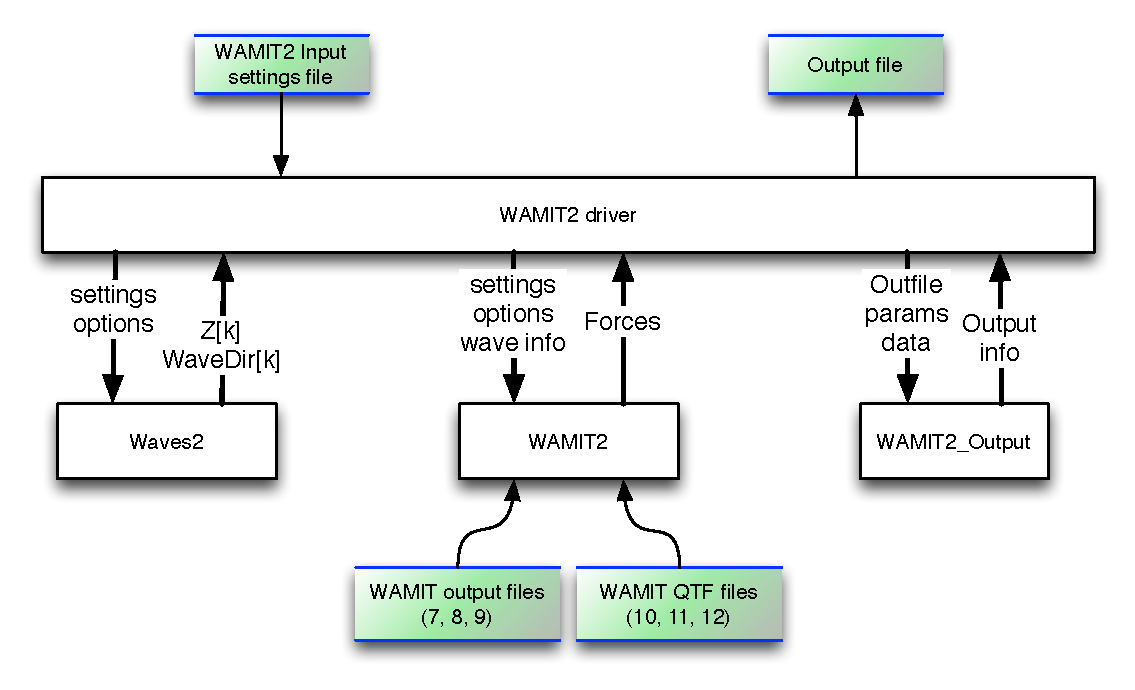
\includegraphics[width=.9\textwidth]{chaps/figures/WAMIT2_Dev.pdf}
      \caption{Information flow to and from the WAMIT2 module. The green boxes indicate information or files passed into or out of the module.\label{fig:W2Interface}}
\end{figure}


\endinput


\begin{figure}
   \centering
      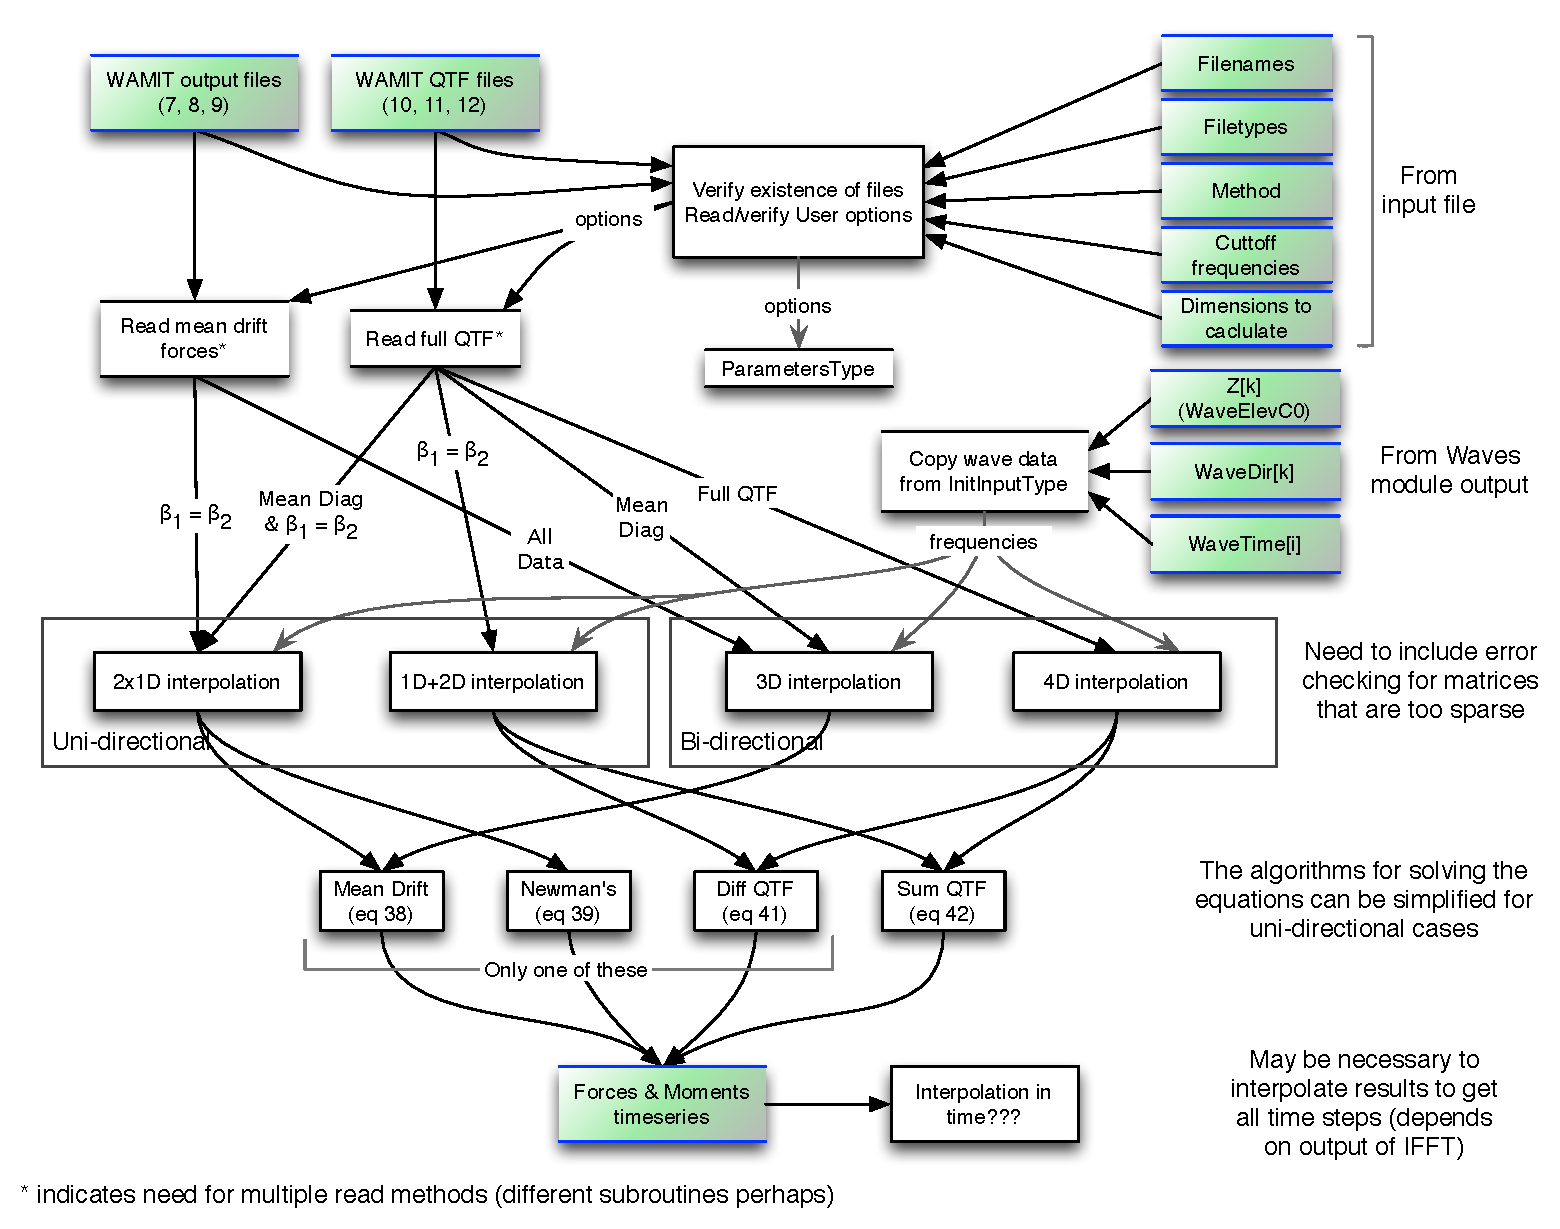
\includegraphics[width=.9\textwidth]{chaps/figures/HydroDyn_2nd_order--WAMIT2_Init.pdf}
      \caption{Information flow within the Init routine in the WAMIT2 sub-module. {\bfseries OUTDATED:} Diagram for parse then interpolate method -- interpolation is done at each step in the equation solver using a 3D and 4D interpolation.\label{fig:InitInformationFlow}}
\end{figure}

\section{Input information}
The wave information in the frequency domain will need to be passed into the WAMIT2 module. This is available at the platform reference point as \emph{WaveElevCO} in the \emph{InitOutputType} from the Waves module (calculated on line 1322 of \emph{Waves.f90}, revision 98 in \emph{branches/HydroDyn\_Modularization/Source}). In the code, the frequency is given as $\omega = k \Delta \omega$, the index times the frequency step. Since $k$ is positive, there are no negative frequencies. Tiago assumed in equation 23 of his write-up that there are negative frequencies, so I assume he included them simply for completeness (I don't think it makes sense to worry about negative frequencies since that can be accounted for by direction).

At present, the Waves module only uses a single direction for the waves. So, an array of wave directions does not exist (scalar value at present). That will need to be added to the Waves module at some point.

\section{File reading}
The WAMIT files to be read in can have an extension of .7, .8, .9, .10d, .10s, .11d, .11s, .12d, or .12s. The .7 extension is only available for files generated with WAMIT 7, not WAMIT 6.1s or 6.4, so that may need to be checked.
The entirety of the files is read in and stored in memory.  This involves several passes through the file to figure out how frequency and wave direction components are present in the file, allocate the storage, then read everything in at once.

\section{Calculations}
The calculations are outlined elsewhere in this document.

\section{Init returned information}
%FIXME: Jason thinks this should be $N' = 2(N+1)$ instead of $N$.  I need to double check, but I think my notation has $N'$ and $N$ switched.  I may wish to change this.
The returned information will be an array of forces and moments at specific timesteps (ideally the same as those returned by the WAMIT routine). I suspect that it will be least confusing to return a $6\times N$ array (3 forces, 3 moments, $N$ timesteps) regardless of which forces are calculated. The unrequested ones will just be set to zero. I will have to look at the WAMIT module that Greg worked on to see how he output these forces -- I think they are on a single point mesh.

\section{CalcOutput routine}
This routine will interpolate the force data created by the Init routine in order to get the forces at intermediate timesteps. It may not be necessary to interpolate at all timesteps since the Init routine calculates the forces for all known timesteps at the start of the FAST simulation. However, it might be necessary to interpolate for other timesteps depending on the coupling used in FAST.

\section{HydroDyn modifications/considerations}

\begin{itemize}
   \item{2nd order won't work for certain WaveMod cases because the $Z[k]$ won't be known (i.e. \emph{WaveMod}~$= 5$ for \emph{GH\_BladedWaves\_Init}). Cases to check are \emph{WaveMod} $= \{0,4,5\}$\todo{update from WAMIT.f90}. This should be checked for at the HydroDyn level.  This may need to be checked in {\tt WAMIT2.f90} (it is checked in {\tt WAMIT.f90}).}
\end{itemize}


\endinput
\section{Program Outline}
\subsection{WAMIT2\_Init}
\label{sec:WAMIT2Init}
\todo[inline]{Add in a check on the WaveMod.  See WAMIT.f90 line ~894 ({\tt InitInp\%WaveMod} case)}
\begin{itemize}
   \item{Check inputs}\todo{Change all these to case structures}
   \begin{itemize}
      \item{Values of \emph{MnDrift}, \emph{NewmanApp}, \emph{DiffQTF}, and \emph{SumQTF}}
      \item{Size of \emph{WaveTime}, \emph{WaveElevC0}, and \emph{WaveDir} arrays}
      \item{Cutoff frequencies make sense}
      \item{Existence of WAMIT files}
   \end{itemize}
   \item{Copy input info into WAMIT2\_Parameters}
   \item{Read and parse input files}
   \begin{itemize}
      \item{Mean Drift Force files (\{\emph{MnDrift} || \emph{NewmanApp}\} = \{.7, .8, .9\})}
      \begin{itemize}
         \item{\emph{WaveMultiDir} = .FALSE. $\rightarrow$ $\beta1=\beta2$}
         \item{\emph{WaveMultiDir} = .TRUE. $\rightarrow$ All}
      \end{itemize}
      \item{Difference QTF files (\emph{DiffQTF} = \{.10d, .11d, .12d\})}
      \begin{itemize}
         \item{\emph{WaveMultiDir} = .FALSE.}
         \begin{itemize}
            \item{\emph{MnDrift} || \emph{NewmanApp} $\rightarrow$ Mean diaganoal and $\beta_1 = \beta_2$}
            \item{\emph{DiffQTF} $\rightarrow$ $\beta_1 = \beta_2$}
         \end{itemize}
         \item{\emph{WaveMultiDir} = .TRUE.}
         \begin{itemize}
            \item{\emph{MnDrift} $\rightarrow$   Mean diagonal}
            \item{\emph{DiffQTF} $\rightarrow$   Full QTF}
         \end{itemize}
      \end{itemize}
      \item{Sum QTF files (\emph{SumQTF} = \{.10s, .11s, .12s\})}
      \begin{itemize}
         \item{\emph{WaveMultiDir} = .FALSE. $\rightarrow$ $\beta_1 = \beta_2$}
         \item{\emph{WaveMultiDir} = .TRUE. $\rightarrow$ Full QTF}
      \end{itemize}
   \end{itemize}
   \item{Interpolation}
   \begin{itemize}
      \item{Diff frequency}
      \begin{itemize}
         \item{\emph{WaveMultiDir} = .FALSE.}
         \begin{itemize}
            \item{\emph{MnDrift} || \emph{NewmanApp} $\rightarrow$ 2x1D (\Cref{sec:interp:1d})}
            \item{\emph{DiffQTF} $\rightarrow$   1D+2D (\Cref{sec:interp:1d,sec:interp:2d})}
         \end{itemize}
         \item{\emph{WaveMultiDir} = .TRUE.}
         \begin{itemize}
            \item{\emph{MnDrift} $\rightarrow$   3D (\Cref{sec:interp:3d})}
            \item{\emph{DiffQTF} $\rightarrow$   4D (\Cref{sec:interp:4d})}
         \end{itemize}
      \end{itemize}
      \item{Sum frequency}
      \begin{itemize}
         \item{\emph{WaveMultiDir} = .FALSE. $\rightarrow$  1D+2D (\Cref{sec:interp:1d,sec:interp:2d})}
         \item{\emph{WaveMultiDir} = .TRUE. $\rightarrow$   4D (\Cref{sec:interp:4d})}
      \end{itemize}
   \end{itemize}
   \item{Calculation of forces}
   \begin{itemize}
      \item{\emph{MnDrift} $\ne 0 \rightarrow$     \Cref{eq:MeanDrift}}
      \item{\emph{NewmanApp} $\ne 0 \rightarrow$   \Cref{eq:Newman}}
      \item{\emph{DiffQTF} $\ne 0 \rightarrow$     \Cref{eq:DiffQTF}}
      \item{\emph{SumQTF} $\ne 0 \rightarrow$      \Cref{eq:DiffQTF}}
   \end{itemize}
   \item{Cleanup and exit}
   \begin{itemize}
      \item{Copy data to output mesh}
      \item{Set uncalculated forces to zero}
      \item{Deallocatetemporaryarrays}
   \end{itemize}
\end{itemize}

\subsection{WAMIT2\_CalcOutput routine}
\begin{itemize}
   \item{Interpolate Forces to time DT (may not always be necessary)}
\end{itemize}

\subsection{WAMIT2\_End}
\begin{itemize}
   \item{Destroy data}
\end{itemize}



%\chapter{Programming Development Schedule}
\label{chap:DevSched}

This is a rough outline of the big pieces that need to be completed and tested, along with some rough time estimates.  This schedule is for a 32 hour work week to completion.  This leaves me with an extra day in the week to take care of anything that wasn't finished in the allotted time.

\begin{itemize}
   \item{1 day -- Fix error handling in Greg's code pieces I'm working with (Waves, HydroDyn\_Input)}
   \item{2.5 days -- Impliment multi-directional waves in the waves module in my code base.  Include 2 test cases and resulting plots.  Merge to Greg's at later date.}
   \item{3 days -- finish second order code structure (file reading, WAMIT data storage -- sparce capable, parsing, storage, data handling/passing, all I/O).  This includes all necessary subroutine infrasture with error handling and temporary subroutine placeholders.  Force component flags enabled on my pieces at this point.}
   \item{1 day -- documentation cleanup (diagrams etc), doxygen documentation cleanup}
   \item{2 days -- 3D interpolation (non-sparse) algorithm based on one in InflowWind.  Document and testdata set}
   \item{2 days -- 4D interpolation (non-sparse) algorithm based on 3D above.  Document and testdata set}
   \item{2 days -- Newman Approximation implimentation.  Includes documentation and test dataset}
   \item{2 days -- Mean Drift implimentation.  Includes documentation and test dataset (also for 4D data)}
   \item{1 day -- Diff QTF implimentation (some logic exists in Newman, first term is Mean Drift).  Includes documentation and test dataset (also for 4D)}
   \item{1 day -- Sum QTF implimentation (should be simpler since been through the others).  Includes documentation and test dataset (also 4D test)}
   \item{1 day -- Impliment new equations from Jason for analytic solution (first order)}
   \item{2 days -- Stress test / debug, finalize documentatation}
   \item{1 day -- merge into final release -- will break some of Greg's code with multidirectional waves at this point}
   \item{2 days -- fix multidirectional waves in remaining pieces.  Fix other bugs that come up.}
   \item{0.5 day -- Fix force component issue so that they are used in Greg's code if he hasn't fixed them by the time I get to it (I can proceed with them not implimented)}
\end{itemize}



\endinput


All calculations of the second order forces will be handled by the WAMIT2 module. This module will take the input information including the wave information, files to use, and times the forces are needed at.

\section{Generalized approach}
\begin{enumerate}
   \item{Develop top-level diagram showing information flow between modules (use Tiago's diagram from the bi-directional waves document).}
   \item{{\st{Information flow diagram for development environment for the WAMIT2 sub-module}} (Figure~\ref{fig:W2Interface}).}
   \item{{\st{Information flow diagram for second order forces in the WAMIT2 module}} (Figure~\ref{fig:InitInformationFlow}).}
   \item{Sketch out flow diagram of the calculations. Identify subroutines.}
   \item{\st{Sketch out data storage for second order with bi-directional waves. Create these structures for WAMIT2 in a registry file.}}
   \item{\st{Create the registry using the above information.}}
   \item{\st{HydroDyn Input}}
      \begin{enumerate}
         \item{\st{Add inputs to the HydroDyn file}}
         \item{\st{Update the HydroDyn input file reading and parsing}}
      \end{enumerate}
   \item{Create basic architecture of WAMIT2\_Init subroutine (pseudo-code outline in the framework).}
      \begin{enumerate}
         \item{File reading}
            \begin{enumerate}
               \item{{Include logic for parsing the data files} (sparse files)}
               \item{\st{Include logic for dealing with option combinations}}
               \item{\st{Write out all the logic for reading the WAMIT files for the second order (see Table 3 and Appendix A of Tiago's writeup).}}
            \end{enumerate}
         \item{Data interpolation routines for input data}
         \item{Calculations (eq's 38, 39, 41, 42)}
      \end{enumerate}
   \item{Create basic architecture of WAMIT2\_CalcOutput subroutine}
      \begin{enumerate}
         \item{Interpolation of resulting force timeseries for timesteps not in the original series.}
      \end{enumerate}
   \item{Get the basic skeleton working/compiling in the framework (just the structure and comments). This will include all the data structures and data passing.}
   \item{Revisit and complete the program and data flow diagrams.}
   \item{Finalize pseudo-code.}
   \item{Replace the pseudo-code with real code.}
   \item{Test. Develop test cases (occurs during previous step).}
\end{enumerate}

In addition to the above methodology, the calculations and data structures will be implemented in such a way so as to include the bi-directional waves.




% bibliography
\cleardoublepage
%\bibliographystyle{nrel}
\bibliographystyle{unsrt}
%\bibintoc
\label{sec:Bib}
\bibliography{bibliography}


%\appendix
%\chapter{Derivation of \nth{2}-order force equations}
\label{app:2ndOrdDeriv}

If I ever get around to it, I will work out the derivations on my own (non-work) time and put them here.

%\chapter{Data preparation schemes for calculations}
\label{app:DataPrepScheme}

There are several ways to take the WAMIT data and prepare it for the calculations.  The first scheme (which Tiago described in one of his documents) is to parse out the relevent data, then interpolate to find the data necessary for the calcution.  Second scheme is to interpolate all the data first, then parse out the relevant parts.  These two schemes lend themselves to a matrix driven data processing such as might occur in MATLAB based code.

The third schemes, which is used in this module of \HD is to interpolate the sorted WAMIT data during the calculations themselves. This scheme presents the lowest memory usage of the three schemes as only the sorted raw data must be stored.  The interpolation step is then performed within the loops of the calculation.  The interpolated data is not kept as it is not needed afterwards.

%FIXME: add diagram from the notebook, p. 142

\section{Parse then Interpolate}
One method is to take the sorted data from the WAMIT file and parse out only the pieces of interest.  For example, a full second order QTF WAMIT file (.12d for example) might only be used in Newman's approximation.  In this case, only terms where $\omega_m = \omega_n$ and $\beta_1 = \beta_2$ are kept.  It would be possible to only keep these values and put them in a simplified matrix dependent on $\omega$ and $\beta$.  This could then be sent through two one dimensional interpolations (one interpolation on each dimension). In this manner, different interpolations would be done depending on which calculation method we were using.

The advantage with this data preparation scheme is that we can keep a small set of data and we can use simpler interpolations for some of the calculation methods.  The disadvantage is that we end up imposing that the values of the $\omega_m$ terms must be identical to the values of the $\omega_n$ terms (otherwise there would be no $\omega_m = \omega_n$ terms to keep).  This would also be true for the $\beta$ terms.  

\begin{figure}[ht]
   \begin{center}
      \beginpgfgraphicnamed{MeanDrift.Flowchart}
         %%% This approach is not correct: we don't want to parse first.  We can do the parsing as part of the loop and interpolate within the loop.
\begin{tikzpicture}

% temporary node for the sectioning labels
\node[tempnode]
      (TmpNode) {};

% WAMIT 1st order
\node[info,right of=TmpNode,node distance=30mm,text width=19mm,text centered] 
      (W1Data) {Read \nth{1}~order WAMIT~output (.7~.8~.9)};

\node[process,below of=W1Data,node distance=13mm]
      (W1Sort) {Sort data};
   \draw[cl] (W1Data) -- (W1Sort);

\node[process,below of=W1Sort,node distance=12mm]
      (W1Convert) {Convert $\tau \rightarrow \omega$};
   \draw[cl] (W1Sort) -- (W1Convert);

\node[info,below of=W1Convert,node distance=12mm]
      (W1Info) {Raw \nth{1} order data};
   \draw[cl] (W1Convert) -- (W1Info);

\node[annotation,right of=W1Info,node distance=25mm,text centered, text width=15mm]
      (W1InfoSize) {$6 \times n_\omega \times n_{\beta_1} \times n_{\beta_2}$};
   \draw[gray] (W1Info) -- (W1InfoSize);

% unidirectional
   \node[process]
         (W1UniParse) at ($(W1Info)+(-13mm,-15mm)$) {$\beta_1=\beta_2$ terms};
      \draw[cl] (W1Info) -- (W1UniParse);
   \node[annotation,text centered, text width=15mm]
         (W1UniParseSize) at ($(W1UniParse)+(-5mm,-8mm)$) {$6 \times n_\omega \times n_{\beta}$};
      \draw[gray] (W1UniParse) -- (W1UniParseSize);
   
% multidirectional
   \node[process] 
         (W1BiParse) at ($(W1Info)+(13mm,-15mm)$)  {all terms};
      \draw[cl] (W1Info) -- (W1BiParse);


%WAMIT 2nd
\node[info,right of=W1Data,node distance=60mm,text width=21mm,text centered] 
      (W2Data) {Read \nth{2}~order WAMIT~output (.10d~.11d~.12d)};

\node[process,below of=W2Data,node distance=13mm]
      (W2Sort) {Sort data};
   \draw[cl] (W2Data) -- (W2Sort);

\node[process,below of=W2Sort,node distance=12mm]
      (W2Convert) {Convert $\tau \rightarrow \omega$};
   \draw[cl] (W2Sort) -- (W2Convert);

\node[info,below of=W2Convert,node distance=12mm]
      (W2Info) {Raw \nth{2} order data};
   \draw[cl] (W2Convert) -- (W2Info);

\node[annotation,right of=W2Info,node distance=27mm,text centered, text width=18mm]
      (W2InfoSize) {$6 \times n_{\omega_1} \times n_{\omega_2} \times n_{\beta_1} \times n_{\beta_2}$};
   \draw[gray] (W2Info) -- (W2InfoSize);

% unidirectional
   \node[process,text width=24mm,text centered]
         (W2UniParse) at ($(W2Info)+(-15mm,-15mm)$) {$\beta_1=\beta_2$ when $\omega_1=\omega_2$ terms};
      \draw[cl] (W2Info) -- (W2UniParse);
   \node[annotation,text centered, text width=15mm]
         (W2UniParseSize) at ($(W2UniParse)+(1mm,-9.5mm)$) {$6 \times n_\omega \times n_{\beta}$};
      \draw[gray] (W2UniParse) -- (W2UniParseSize);
   
% multidir
   \node[process,text width=24mm,text centered]
         (W2BiParse) at ($(W2Info)+(15mm,-15mm)$) {$\omega_1=\omega_2$ terms};
      \draw[cl] (W2Info) -- (W2BiParse);
   \node[annotation,text centered, text width=15mm]
         (W2BiParseSize) at ($(W2BiParse)+(6mm,-10mm)$) {$6 \times n_\omega \times n_{\beta_1} \times n_{\beta_2}$};
      \draw[gray] (W2BiParse) -- (W2BiParseSize);
   


%%%%%%%%%%%%%%%%%%%%%%
% Interpolation step %

% unidirectional
\node[process,anchor=north]
      (UniInterp1) at ($(W1Data)+(5mm,-70mm)$) {Interpolate $\beta$};
   \draw[cl] (W1UniParse) -- (UniInterp1);
   \draw[cl] (W2UniParse) -- (UniInterp1);

\node[process,below of=UniInterp1]
      (UniInterp2) {Interpolate $\omega$};
   \draw[cl] (UniInterp1) -- (UniInterp2);

%set the background box of unidirectional
\begin{pgfonlayer}{background}
\filldraw[rounded corners=3mm,draw=blue!30!black!35,
            fill=white!80!blue!20!red!20!black!10]
      ($(UniInterp1.north west) +(-12mm,2mm)$) 
         rectangle ($(UniInterp2.south east)+(2mm,-2mm)$);
\end{pgfonlayer}
\node[tempnode,anchor=north,font=\footnotesize,text centered,text width=18mm,rotate=90]
      (UniDir) at ($(UniInterp1.west)!.5!(UniInterp2.west)+(-11mm,0mm)$) {\it{Uni-dir waves}\\(2$\times$1D)};



% multidirectional
\coordinate (tmp) at ($(UniInterp1)!.5!(UniInterp2)$);
\node[process,text width=21mm,text centered,anchor=center]
      (BiInterp1) at ($(W2Data |-  tmp) +(-0mm,0mm)$) {Interpolate 3D over $\omega, \beta_1, \beta_2$};
   \draw[red]  (BiInterp1.north west) -- (BiInterp1.south east);
   \draw[red]  (BiInterp1.north east) -- (BiInterp1.south west);
   \draw[cl,gray!50] (W1BiParse) -- (BiInterp1);
   \draw[cl,gray!50] (W2BiParse) -- (BiInterp1);

%set the background box of Multidirectional
\begin{pgfonlayer}{background}
\filldraw[rounded corners=3mm,draw=blue!30!black!35,
            fill=white!80!blue!20!red!20!black!10]
      ($(BiInterp1.north west) +(-12mm,2mm)$) 
         rectangle ($(BiInterp1.south east)+(2mm,-2mm)$);
\end{pgfonlayer}
\node[tempnode,anchor=north,font=\footnotesize,text centered,text width=18mm,rotate=90]
      (MultDir) at ($(BiInterp1.west)+(-11mm,0mm)$) {\it{Multi-dir waves} (\Cref{sec:interp:3d})};



%%%%%%%%%%%%%%%%%%%%%%
% Transfer function
\node[info]
      (TransFunc) at ($(UniInterp1)!.5!(BiInterp1) + (0mm,-25mm)$) {$F^\text{Drift}_k(\omega)$};
   \draw[cl,gray!50] (BiInterp1) -- (TransFunc);
   \draw[cl] (UniInterp2) -- (TransFunc);
\node[annotation,right of=TransFunc,node distance=20mm]
      (TransFuncA) {$6 \times N/2$ terms};
   \draw[gray] (TransFunc) -- (TransFuncA);


% Equation
\node[process,below of=TransFunc]
      (EQ) {\Cref{eq:MeanDrift}};
   \draw[cl] (TransFunc) -- (EQ);



%output
\node[info,below of=EQ,text width=21mm,text centered,node distance=14mm]
      (Output) {Forces and moments to apply to point mesh};
   \draw[cl] (EQ) -- (Output);





%% draw some lines along the side for marking what parts do what
\coordinate (tmp1) at ($(TmpNode |- W1Data)+(0mm,7mm)$);
\coordinate (tmp2) at ($(TmpNode |- W1Info)+(0mm,-5mm)$);
\draw[black]
      ($(tmp1)+(3mm,0mm)$) -- (tmp1) -- (tmp2) 
         node[midway,above,sloped,rotate=180,font=\small] {Data reading} -- +(3mm,0mm);

\coordinate (tmp1) at ($(TmpNode |- W1UniParse)+(0mm,5mm)$);
\coordinate (tmp2) at ($(TmpNode |- W1UniParse)+(0mm,-5mm)$);
\draw[black]
      ($(tmp1)+(3mm,0mm)$) -- (tmp1) -- (tmp2) 
            node[midway,above,sloped,rotate=180,font=\small] {Parsing}-- +(3mm,0mm);

\coordinate (tmp1) at ($(TmpNode |- UniInterp1)+(0mm,5mm)$);
\coordinate (tmp2) at ($(TmpNode |- UniInterp2)+(0mm,-5mm)$);
\draw[black,text width=21mm,text centered]
      ($(tmp1)+(3mm,0mm)$) -- (tmp1) -- (tmp2) 
            node[midway,above,sloped,rotate=180,font=\small] {Interpolation (\Cref{chap:Algorithm})}-- +(3mm,0mm);

   
\end{tikzpicture}
\endinput


      \endpgfgraphicnamed
   \end{center}
\caption{Flow diagram for the mean drift calculation method using the parse then interpolate scheme.  $\tau$ is the period, $\omega$ is the corresponding frequency, and $\beta$ is the wave direction.  The \nth{1} and \nth{2} order {\tt WAMIT} output files are read in and arranged in ascending order within the {\tt WAMIT2\_Init} routine (\Cref{sec:WAMIT2Init}).  See text for how to solve the equation. See \Cref{chap:WamitOutput} for requirements on which WAMIT output files can be used.
   \label{fig:MeanDrift:Flowchart:ParseInterp}
}
\end{figure}

\begin{figure}[ht]
   \begin{center}
      \beginpgfgraphicnamed{Newman.Flowchart}
         \begin{tikzpicture}

% temporary node for the sectioning labels
\node[tempnode]
      (TmpNode) {};

% WAMIT 1st order
\node[process,right of=TmpNode,node distance=30mm,text width=25mm,text centered] 
      (W1Get) {Read \nth{1}~order WAMIT~output (.7~.8~.9) (\Cref{sec:WamitOuput:Read})};

\node[info,below of=W1Get,node distance=20mm,text width=25mm,text centered]
      (W1Data) {3D matrix\\(possibly sparse)\\$F^\text{-}_k(\omega,\beta_1,\beta_2)$};
   \draw[cl] (W1Get) -- (W1Data);



%WAMIT 2nd
\node[process,right of=W1Get,node distance=60mm,text width=25mm,text centered] 
      (W2Get) {Read \nth{2}~order WAMIT~output (.10d~.11d~.12d) (\Cref{sec:WamitOuput:Read})};

\node[info,below of=W2Get,node distance=20mm,text width=25mm,text centered]
      (W2Data) {4D matrix\\(possibly sparse)\\$F^\text{-}_k(\omega_1,\omega_2,\beta_1,\beta_2)$};
   \draw[cl] (W2Get) -- (W2Data);

%Equation
\node[anchor=center,process]
      (Equation)  at ($(W1Data)!.5!(W2Data)+(0mm,-55mm)$) {$A_m A^*_m ~ F^\text{-}_k(\omega_{m},\omega_{m},\beta_{m},\beta_{m})$};

\draw[red] ($(Equation)+(6mm,0mm)$) ellipse [x radius=17mm, y radius=5mm];

%Solver
\begin{pgfonlayer}{background}
   \filldraw[rounded corners=3mm,draw=blue!30!black!35,
            fill=white!80!blue!20!red!20!black!10]
                        ($(Equation.north west) +(-15mm,34mm)$) coordinate (SolverBoxNW)
            rectangle   ($(Equation.south east)+(5mm,-8mm)$)   coordinate (SolverBoxSE);
   %put box around the equation set
   \draw[rounded corners=1mm,draw=black,thin]
                        ($(Equation.north west) +(-13mm,5mm)$)
            rectangle   ($(Equation.south east)+(2mm,-5mm)$);

   \node[anchor=north west] at ($(SolverBoxNW.north west) +(1mm,-1mm)$) {Solver};
   \node[anchor=east,font=\Huge] (tmp) at ($(Equation.west)+(0mm,0mm)$) {$\sum$};
   \node[anchor=north,font=\footnotesize] at ($(tmp.south)+(0mm,2.0mm)$) {$m_{\omega_\text{lo-d}}$};
   \node[anchor=south,font=\footnotesize] at ($(tmp.north)+(0mm,-2.0mm)$) {$m_{\omega_\text{hi-d}}$};
\end{pgfonlayer}

%Solver inputs
\node[info,text width=15mm,text centered] (SolveInput) at ($(SolverBoxNW |- Equation)+(-20mm,0mm)$) {$Z(\omega,\beta)$\\Limits};
   \draw[cl] (SolveInput) -- ($(SolverBoxNW |- Equation)$);

%Solver results
\node[info,text width=15mm,text centered] (SolveResults) at ($(SolverBoxSE |- Equation)+(20mm,0mm)$) {$F^{\text{-} (2)}_{\text{ex}~k}$};
   \draw[cl] ($(SolverBoxSE |- Equation)$) -- (SolveResults);



%Interpolation
\node[process,text width=25mm,text centered] (Interpolate) at ($(Equation.north)+(0mm,21mm)$) {3D / 4D Interpolation at each $m$th summation step (\Cref{sec:Algorithm:Interp})};
   \draw[cl] (Interpolate.south) -- ($(Equation)+(4mm,5mm)$);
   \draw[cl] (W1Data) -- (Interpolate);
   \draw[cl] (W2Data) -- (Interpolate);


\end{tikzpicture}
\endinput


%% draw some lines along the side for marking what parts do what
\coordinate (tmp1) at ($(TmpNode |- W1Data)+(0mm,7mm)$);
\coordinate (tmp2) at ($(TmpNode |- W1Info)+(0mm,-5mm)$);
\draw[black]
      ($(tmp1)+(3mm,0mm)$) -- (tmp1) -- (tmp2) 
         node[midway,above,sloped,rotate=180,font=\small] {Data reading} -- +(3mm,0mm);

\coordinate (tmp1) at ($(TmpNode |- W1UniParse)+(0mm,5mm)$);
\coordinate (tmp2) at ($(TmpNode |- W1UniParse)+(0mm,-5mm)$);
\draw[black]
      ($(tmp1)+(3mm,0mm)$) -- (tmp1) -- (tmp2) 
            node[midway,above,sloped,rotate=180,font=\small] {Parsing}-- +(3mm,0mm);

\coordinate (tmp1) at ($(TmpNode |- UniInterp1)+(0mm,5mm)$);
\coordinate (tmp2) at ($(TmpNode |- UniInterp2)+(0mm,-5mm)$);
\draw[black,text width=21mm,text centered]
      ($(tmp1)+(3mm,0mm)$) -- (tmp1) -- (tmp2) 
            node[midway,above,sloped,rotate=180,font=\small] {Interpolation (\Cref{chap:Algorithm})}-- +(3mm,0mm);

   
\end{tikzpicture}
\endinput


      \endpgfgraphicnamed
   \end{center}
\caption{Flow diagram for the Newman's approximation method using the parse then interpolate scheme.  $\tau$ is the period, $\omega$ is the corresponding frequency, and $\beta$ is the wave direction.  The \nth{1} and \nth{2} order {\tt WAMIT} output files are read in and arranged in ascending order within the {\tt WAMIT2\_Init} routine (\Cref{sec:WAMIT2Init}).
   \label{fig:Newman:Flowchart:ParseInterp}
}
\end{figure}

\begin{figure}[ht]
   \begin{center}
      \beginpgfgraphicnamed{DiffQTF.Flowchart}
         \begin{tikzpicture}

% temporary node for the sectioning labels
\node[tempnode]
      (TmpNode) {};


%WAMIT 2nd
\node[info,right of=TmpNode,node distance=50mm,text width=21mm,text centered] 
      (W2Data) {Read \nth{2}~order WAMIT~output (.10d~.11d~.12d)};

\node[process,below of=W2Data,node distance=13mm]
      (W2Sort) {Sort data};
   \draw[cl] (W2Data) -- (W2Sort);

\node[process,below of=W2Sort,node distance=12mm]
      (W2Convert) {Convert $\tau \rightarrow \omega$};
   \draw[cl] (W2Sort) -- (W2Convert);

\node[info,below of=W2Convert,node distance=12mm]
      (W2Info) {Raw \nth{2} order data};
   \draw[cl] (W2Convert) -- (W2Info);

% unidirectional
   \node[process,text width=24mm,text centered]
         (W2UniParse) at ($(W2Info)+(-15mm,-15mm)$) {$\beta_1=\beta_2$ terms};
      \draw[cl] (W2Info) -- (W2UniParse);
   
% multidir
   \node[process,text width=24mm,text centered]
         (W2BiParse) at ($(W2Info)+(15mm,-15mm)$) {Full QTF};
      \draw[cl] (W2Info) -- (W2BiParse);


%%%%%%%%%%%%%%%%%%%%%%
% Interpolation step %

% unidirectional
\node[process,anchor=north]
      (UniInterp1) at ($(W2Data)+(-20mm,-65mm)$) {Interpolate $\beta$};
   \draw[cl] (W2UniParse) -- (UniInterp1);

\node[process,below of=UniInterp1]
      (UniInterp2) {Interpolate $\omega_1, \omega_2$};
   \draw[cl] (UniInterp1) -- (UniInterp2);

%set the background box of unidirectional
\begin{pgfonlayer}{background}
\filldraw[rounded corners=3mm,draw=blue!30!black!35,
            fill=white!80!blue!20!red!20!black!10]
      ($(UniInterp1.north west) +(-14mm,2mm)$) 
         rectangle ($(UniInterp2.south east)+(2mm,-2mm)$);
\end{pgfonlayer}
\node[tempnode,anchor=north,font=\footnotesize,text centered,text width=20mm,rotate=90]
      (UniDir) at ($(UniInterp1.west)!.5!(UniInterp2.west)+(-11.5mm,0mm)$) {\it{Uni-dir waves} (\Cref{sec:interp:1d,sec:interp:2d})};



% multidirectional
\coordinate (tmp) at ($(UniInterp1)!.5!(UniInterp2)$);
\node[process,text width=21mm,text centered,anchor=center]
      (BiInterp1) at ($(W2Data |-  tmp) +(25mm,0mm)$) {Interpolate 4D over $\omega_1, \omega_2, \beta_1, \beta_2$};
   \draw[cl] (W2BiParse) -- (BiInterp1);

%set the background box of Multidirectional
\begin{pgfonlayer}{background}
\filldraw[rounded corners=3mm,draw=blue!30!black!35,
            fill=white!80!blue!20!red!20!black!10]
      ($(BiInterp1.north west) +(-12mm,3mm)$) 
         rectangle ($(BiInterp1.south east)+(2mm,-3mm)$);
\end{pgfonlayer}
\node[tempnode,anchor=north,font=\footnotesize,text centered,text width=18mm,rotate=90]
      (MultDir) at ($(BiInterp1.west)+(-11mm,0mm)$) {\it{Multi-dir waves} (\Cref{sec:interp:4d})};



%%%%%%%%%%%%%%%%%%%%%%
% Transfer function
\node[info]
      (TransFunc) at ($(W2Data) + (0mm,-95mm)$) {$F^{-}_k(\omega_m,\omega_n)$};
   \draw[cl] (BiInterp1) -- (TransFunc);
   \draw[cl] (UniInterp2) -- (TransFunc);

% Equation
\node[process,below of=TransFunc]
      (EQ) {\Cref{eq:DiffQTF}};
   \draw[cl] (TransFunc) -- (EQ);



%output
\node[info,below of=EQ,text width=21mm,text centered,node distance=14mm]
      (Output) {Forces and moments to apply to point mesh};
   \draw[cl] (EQ) -- (Output);





%% draw some lines along the side for marking what parts do what
\coordinate (tmp1) at ($(TmpNode |- W2Data)+(0mm,7mm)$);
\coordinate (tmp2) at ($(TmpNode |- W2Info)+(0mm,-5mm)$);
\draw[black]
      ($(tmp1)+(3mm,0mm)$) -- (tmp1) -- (tmp2) 
         node[midway,above,sloped,rotate=180,font=\small] {Data reading} -- +(3mm,0mm);

\coordinate (tmp1) at ($(TmpNode |- W2UniParse)+(0mm,5mm)$);
\coordinate (tmp2) at ($(TmpNode |- W2UniParse)+(0mm,-5mm)$);
\draw[black]
      ($(tmp1)+(3mm,0mm)$) -- (tmp1) -- (tmp2) 
            node[midway,above,sloped,rotate=180,font=\small] {Parsing}-- +(3mm,0mm);

\coordinate (tmp1) at ($(TmpNode |- UniInterp1)+(0mm,5mm)$);
\coordinate (tmp2) at ($(TmpNode |- UniInterp2)+(0mm,-5mm)$);
\draw[black,text width=21mm,text centered]
      ($(tmp1)+(3mm,0mm)$) -- (tmp1) -- (tmp2) 
            node[midway,above,sloped,rotate=180,font=\small] {Interpolation (\Cref{chap:Algorithm})}-- +(3mm,0mm);

   
\end{tikzpicture}
\endinput


      \endpgfgraphicnamed
   \end{center}
\caption{Flow diagram for the full difference QTF method using the parse then interpolate scheme.  $\tau$ is the period, $\omega$ is the corresponding frequency, and $\beta$ is the wave direction.  The \nth{1} and \nth{2} order {\tt WAMIT} output files are read in and arranged in ascending order within the {\tt WAMIT2\_Init} routine (\Cref{sec:WAMIT2Init}).
   \label{fig:DiffQTF:Flowchart:ParseInterp}
}
\end{figure}

\begin{figure}[ht]
   \begin{center}
      \beginpgfgraphicnamed{DiffQTF.Flowchart}
         %%% This approach is not correct: we don't want to parse first.  We can do the parsing as part of the loop and interpolate within the loop.
\begin{tikzpicture}

% temporary node for the sectioning labels
\node[tempnode]
      (TmpNode) {};


%WAMIT 2nd
\node[info,right of=TmpNode,node distance=50mm,text width=21mm,text centered] 
      (W2Data) {Read \nth{2}~order WAMIT~output (.10s~.11s~.12s)};

\node[process,below of=W2Data,node distance=13mm]
      (W2Sort) {Sort data};
   \draw[cl] (W2Data) -- (W2Sort);

\node[process,below of=W2Sort,node distance=12mm]
      (W2Convert) {Convert $\tau \rightarrow \omega$};
   \draw[cl] (W2Sort) -- (W2Convert);

\node[info,below of=W2Convert,node distance=12mm]
      (W2Info) {Raw \nth{2} order data};
   \draw[cl] (W2Convert) -- (W2Info);

% unidirectional
   \node[process,text width=24mm,text centered]
         (W2UniParse) at ($(W2Info)+(-15mm,-15mm)$) {$\beta_1=\beta_2$ terms};
      \draw[cl] (W2Info) -- (W2UniParse);
   
% multidir
   \node[process,text width=24mm,text centered]
         (W2BiParse) at ($(W2Info)+(15mm,-15mm)$) {Full QTF};
      \draw[cl] (W2Info) -- (W2BiParse);


%%%%%%%%%%%%%%%%%%%%%%
% Interpolation step %

% unidirectional
\node[process,anchor=north]
      (UniInterp1) at ($(W2Data)+(-20mm,-65mm)$) {Interpolate $\beta$};
   \draw[cl] (W2UniParse) -- (UniInterp1);

\node[process,below of=UniInterp1]
      (UniInterp2) {Interpolate $\omega_1, \omega_2$};
   \draw[cl] (UniInterp1) -- (UniInterp2);

%set the background box of unidirectional
\begin{pgfonlayer}{background}
\filldraw[rounded corners=3mm,draw=blue!30!black!35,
            fill=white!80!blue!20!red!20!black!10]
      ($(UniInterp1.north west) +(-14mm,2mm)$) 
         rectangle ($(UniInterp2.south east)+(2mm,-2mm)$);
\end{pgfonlayer}
\node[tempnode,anchor=north,font=\footnotesize,text centered,text width=20mm,rotate=90]
      (UniDir) at ($(UniInterp1.west)!.5!(UniInterp2.west)+(-11.5mm,0mm)$) {\it{Uni-dir waves}\\(1D, 2D)};



% multidirectional
\coordinate (tmp) at ($(UniInterp1)!.5!(UniInterp2)$);
\node[process,text width=21mm,text centered,anchor=center]
      (BiInterp1) at ($(W2Data |-  tmp) +(25mm,0mm)$) {Interpolate 4D over $\omega_1, \omega_2, \beta_1, \beta_2$};
   \draw[cl] (W2BiParse) -- (BiInterp1);

%set the background box of Multidirectional
\begin{pgfonlayer}{background}
\filldraw[rounded corners=3mm,draw=blue!30!black!35,
            fill=white!80!blue!20!red!20!black!10]
      ($(BiInterp1.north west) +(-12mm,3mm)$) 
         rectangle ($(BiInterp1.south east)+(2mm,-3mm)$);
\end{pgfonlayer}
\node[tempnode,anchor=north,font=\footnotesize,text centered,text width=18mm,rotate=90]
      (MultDir) at ($(BiInterp1.west)+(-11mm,0mm)$) {\it{Multi-dir waves} (\Cref{sec:interp:4d})};



%%%%%%%%%%%%%%%%%%%%%%
% Transfer function
\node[info]
      (TransFunc) at ($(W2Data) + (0mm,-95mm)$) {$F^\text{+}_k(\omega_m,\omega_n)$};
   \draw[cl] (BiInterp1) -- (TransFunc);
   \draw[cl] (UniInterp2) -- (TransFunc);

% Equation
\node[process,below of=TransFunc]
      (EQ) {\Cref{eq:SumQTF}};
   \draw[cl] (TransFunc) -- (EQ);



%output
\node[info,below of=EQ,text width=21mm,text centered,node distance=14mm]
      (Output) {Forces and moments to apply to point mesh};
   \draw[cl] (EQ) -- (Output);





%% draw some lines along the side for marking what parts do what
\coordinate (tmp1) at ($(TmpNode |- W2Data)+(0mm,7mm)$);
\coordinate (tmp2) at ($(TmpNode |- W2Info)+(0mm,-5mm)$);
\draw[black]
      ($(tmp1)+(3mm,0mm)$) -- (tmp1) -- (tmp2) 
         node[midway,above,sloped,rotate=180,font=\small] {Data reading} -- +(3mm,0mm);

\coordinate (tmp1) at ($(TmpNode |- W2UniParse)+(0mm,5mm)$);
\coordinate (tmp2) at ($(TmpNode |- W2UniParse)+(0mm,-5mm)$);
\draw[black]
      ($(tmp1)+(3mm,0mm)$) -- (tmp1) -- (tmp2) 
            node[midway,above,sloped,rotate=180,font=\small] {Parsing}-- +(3mm,0mm);

\coordinate (tmp1) at ($(TmpNode |- UniInterp1)+(0mm,5mm)$);
\coordinate (tmp2) at ($(TmpNode |- UniInterp2)+(0mm,-5mm)$);
\draw[black,text width=21mm,text centered]
      ($(tmp1)+(3mm,0mm)$) -- (tmp1) -- (tmp2) 
            node[midway,above,sloped,rotate=180,font=\small] {Interpolation (\Cref{chap:Algorithm})}-- +(3mm,0mm);

   
\end{tikzpicture}
\endinput


      \endpgfgraphicnamed
   \end{center}
\caption{Flow diagram for the full summation QTF method using the parse then interpolate scheme.  $\tau$ is the period, $\omega$ is the corresponding frequency, and $\beta$ is the wave direction.  The \nth{1} and \nth{2} order {\tt WAMIT} output files are read in and arranged in ascending order within the {\tt WAMIT2\_Init} routine (\Cref{sec:WAMIT2Init}).
   \label{fig:SumQTF:Flowchart:ParseInterp}
}
\end{figure}

\clearpage

\section{Interpolate then parse}
Another scheme is to take the sorted WAMIT data and interpolate for all possible values of $\omega_m, \omega_n, \beta_1,$ and $\beta_2$ before selecting out the specific values wanted for the calculation.  The parsing step would then be perfomed afterwards to select only the values needed for the calculation.  This scheme has a very large memory footprint and large amount of processing time spent on the interpolation.  This scheme would be appropriate if the fully interpolated data set was used a large number of times during a \HD simulation, or if a complicated interpolation scheme was used (such as a four dimensional FFT interpolation).  However, in our implimention of \HD, only a small portion of the data would be used, and only used once during initialization.  This scheme is therefore unecessarily complicated for our purposes.

\section{Interpolate during calculation}
This scheme is used in the \modname{WAMIT2} module to perform the interplation of the sorted WAMIT data at each step of the calculation.  The calculations each require summations over a range of frequencies, or inverse discrete Fourier transforms over a range of frequencies.  The WAMIT data can be categorized as either three-dimensional, or four-dimensional depending on what WAMIT output files were used.  At each step of a summation loop, a call can be made to a subroutine that will interpolate the sorted WAMIT data for the particular $F^\pm(\omega_m,\omega_n,\beta_m,\beta_n)$ value required.  There might be a slight computational penalty for calling the interpolation scheme multiple times for sequential points.  Overall this scheme has the advantage that the returned value could be stored in a temporary variable and immediately used.  This limits the memory usage since the complete interpolated multi-dimensional matrix is not stored.



\end{document}
